\documentclass[12pt,openright,
chapter=TITLE, % títulos de capítulos convertidos em letras maiúsculas
section=TITLE, % títulos de seções convertidos em letras maiúsculas
subsection=title, % títulos de subseções convertidos em letras maiúsculas
%fleqn, %fórmulas são vistas alinhadas pela esquerda ao invés de centralizadas. 
oneside,a4paper,english,french,spanish]{abntex2}

\usepackage{cmap}	
\usepackage{lmodern}	
\usepackage[brazil]{babel}
\usepackage[utf8]{inputenc}		
\usepackage{lastpage}		
%\usepackage{indentfirst}   	% Faz com que o 1º paragrafo de cada seção não fique recuado a esquerda
\usepackage{color}	
\usepackage{graphicx}	
\usepackage{units}
\usepackage[brazilian,hyperpageref]{backref}
\usepackage[alf,bibjustif,recuo=0.0cm]{abntex2cite} % bibjustif justifica a referência.
\usepackage{bold-extra}
\usepackage{eso-pic}
\usepackage{empheq,amsmath}
\usepackage{lipsum}
\usepackage{setspace}
\usepackage{verbatim}
\usepackage{float}
\usepackage{listings}


% CONFIGURAÇÕES DE PACOTES
% ---
% Configurações do pacote backref
% Usado sem a opção hyperpageref de backref
%\renewcommand{\backrefpagesname}{Citado na(s) página(s):~}
% Texto padrão antes do número das páginas
%\renewcommand{\backref}{}
% Define os textos da citação
%\renewcommand*{\backrefalt}[4]{
%	\ifcase #1 %
%		Nenhuma citação no texto.%
%	\or
%		Citado na página #2.%
%	\else
%		Citado #1 vezes nas páginas #2.%
%	\fi}%

\newcommand{\curso}[1]{\def\imprimircurso{#1}}

\newcommand{\departamento}[1]{\def\imprimirdepartamento{#1}}
\newcommand{\Title}[1]{\def\imprimirTitle{#1}}


\newcommand{\palavraChaveUm}[1]{\def\imprimirpalavrachaveum{#1}}
\newcommand{\palavraChaveDois}[1]{\def\imprimirpalavrachavedois{#1}}
\newcommand{\palavraChaveTres}[1]{\def\imprimirpalavrachavetres{#1}}
\newcommand{\palavraChaveQuatro}[1]{\def\imprimirpalavrachavequatro{#1}}

\newcommand{\palavraChaveUmingles}[1]{\def\imprimirpalavrachaveumingles{#1}}
\newcommand{\palavraChaveDoisingles}[1]{\def\imprimirpalavrachavedoisingles{#1}}
\newcommand{\palavraChaveTresingles}[1]{\def\imprimirpalavrachavetresingles{#1}}
\newcommand{\palavraChaveQuatroingles}[1]{\def\imprimirpalavrachavequatroingles{#1}}


\newcommand{\cdu}[1]{\def\nomecdu{#1}}
\newcommand{\dataDaAprovacao}[1]{\def\imprimirdatadaaprovacao{#1}}

\newcommand{\mes}[1]{\def\imprimirmes{#1}}

\newcommand{\dia}[1]{\def\imprimirdia{#1}}

\newcommand{\publicacao}[1]{\def\imprimirpublicacao {#1}}

\newcommand{\ENDERECO}[1]{\def\imprimirendereco{#1}}

\newcommand{\CEP}[1]{\def\imprimirCEP{#1}}


\newcommand{\membroConvidadoUm}[1]{\def\imprimirmembroconvidadoum{#1}}
\newcommand{\membroConvidadoDois}[1]{\def\imprimirmembroconvidadodois{#1}}
\newcommand{\membroCoorientador}[1]{\def\imprimirmembroCoorientador{#1}}


\newcommand\BackgroundPic{%
	\put(0,0){%
		\parbox[b][\paperheight]{\paperwidth}{%
			\vfill
%			\centering
%			\includegraphics[width=\paperwidth,height=\paperheight,%
%				keepaspectratio]{figuras/capa.eps}%
			\vfill
		}
	}
}

\renewcommand{\imprimircapa}{%
  \begin{capa}
    \center
    \vspace*{0in}
	{\textbf{\imprimirinstituicao}}
	\par
	{\textbf{\imprimirdepartamento}}

	\vspace{2. in}
	{\textbf{\large \imprimirtitulo}}
    	\vspace{0.25 in}
    	\par
         {\textbf{\large \imprimirautor}}
    	\vspace{2. in}

	    \textbf{ORIENTADORA: \imprimirorientador}\\
    	    \textbf{COORIENTADORA: \imprimirmembroCoorientador}\\
   	    \vspace{0.5 in}
	    \textbf{DISSERTAÇÃO DE MESTRADO EM ENGENHARIA BIOMÉDICA}
		
    \vspace*{1.0 in}
    \textbf{PUBLICAÇÃO: \imprimirpublicacao / \imprimirdata }
    \par
    \textbf{\imprimirlocal: \imprimirmes\,-\,\imprimirdata}  
  \end{capa}
}


% Dados pessoais
\autor{Roberto Aguiar Lima}
\departamento{PROGRAMA DE PÓS-GRADUAÇÃO EM ENGENHARIA \\ BIOMÉDICA}
\instituicao{UnB - UNIVERSIDADE DE BRASÍLIA 
		\par
		FGA - FACULDADE UNB GAMA}
		
\local{BRASÍLIA/DF }
\data{2015}
\mes{Setembro}
\dia{30 }
\publicacao{NUMERAÇÃO }
\ENDERECO{Av. Central, Bl. 191, N. 10, N. Bandeirante}
\CEP{71710010}
\cdu{Nº da CDU (biblioteca)}
% Dados do trabalho
\titulo{IMPLEMENTANDO UM SOFTWARE COMO SERVIÇO PARA ANÁLISE E SIMULAÇÃO DE MARCHA HUMANA}
\Title{IMPLEMENTING A SOFTWARE AS A SERVICE FOR HUMAN GAIT ANALYSIS AND SIMULATION}

\orientador{Dra. Lourdes Mattos Brasil}
\membroCoorientador{Dra. Vera Regina Da Silva Marães}
\membroConvidadoUm{Dra. Aline Araujo do Carmo}
\membroConvidadoDois{Dr. Jairo Simão Santana Melo}

\palavraChaveUm {Análise de Marcha}
\palavraChaveDois {Software como Serviço}
\palavraChaveTres {Sistemas Inteligentes}
\palavraChaveQuatro {Simulação}

\palavraChaveUmingles {Gait Analysis}
\palavraChaveDoisingles {Software as a Service}
\palavraChaveTresingles {Inteligent Systems}
\palavraChaveQuatroingles {Simulation}



% Configurações de aparência do PDF final
% alterando o aspecto da cor azul
\definecolor{black}{RGB}{0,0,0}

% informações do PDF
\makeatletter
\hypersetup{
     	%pagebackref=true,
		pdftitle={\@title}, 
		pdfauthor={\@author},
    	pdfsubject={\imprimirpreambulo},
	    pdfcreator={LaTeX with abnTeX2},
		pdfkeywords={abnt}{latex}{abntex}{abntex2}{trabalho acadêmico}, 
		colorlinks=true,       		% false: boxed links; true: colored links
    	linkcolor=black,          		% color of internal links
    	citecolor=black,        		% color of links to bibliography
    	filecolor=magenta,      		% color of file links
		urlcolor=black,
		bookmarksdepth=4
}
\makeatother
% O tamanho do parágrafo é dado por:
\setlength{\parindent}{1.25cm} % Controle do espaçamento entre um parágrafo e outro.

\setlength{\parskip}{0.2cm}  % tente também \onelineskip

% Remova o comentário abaixo para espaçamento simples
%\SingleSpacing

%\setlength{\mathindent}{0.6cm} % Altera o recuo das equações de tiver o pacote fleqn em documentclass

\counterwithout{equation}{chapter} %Faz com que as equações sejam numeradas 1,2,3,...

\counterwithout{table}{chapter} %Faz com que as equações sejam numeradas 1,2,3,...


\counterwithout{footnote}{chapter} %Faz com que as notas de rodapé sejam numeradas 1,2,3,...

%\setlength\afterchapskip{\baselineskip} % Espaçamento entre o título e o texto

\renewcommand{\ABNTEXchapterfontsize}{\fontsize{14}{14}\selectfont} %Letra e tamnaho da fonte do sumário
\renewcommand{\ABNTEXsectionfontsize}{\fontsize{14}{14}\selectfont}
\renewcommand{\ABNTEXsubsectionfontsize}{\fontsize{14}{14}\selectfont}



\makeindex

\begin{document}
\frenchspacing 
\imprimircapa

\begin{folhadeaprovacao}
\begin{center}
    \vspace*{0in}
	{\textbf{\imprimirinstituicao}}
	\par
	{\textbf{\imprimirdepartamento}}

	\vspace{0.5 in}
	{\textbf{\large \imprimirtitulo}}
    	\vspace{0.25 in}
    	\par
         {\textbf{\large \imprimirautor}}
    	\vspace{0.25 in}
\end{center}
\textbf{DISSERTAÇÃO DE MESTRADO SUBMETIDA AO PROGRAMA DE PÓS-GRADUAÇÃO EM ENGENHARIA BIOMÉDICA DA FACULDADE GAMA DA
UNIVERSIDADE DE BRASÍLIA, COMO PARTE DOS REQUISITOS NECESSÁRIOS PARA A OBTENÇÃO DO GRAU DE MESTRE EM
ENGENHARIA BIOMÉDICA.}
\flushleft	
	\vspace{0.5 in}    
    \textbf{APROVADO POR:}\\
    \vspace{0.5 in}    
    \rule{10cm}{.1mm}\\
    {\textbf{Prof. \imprimirorientador} \\ \textbf{(Orientadora)} }\\
    \vspace{0.5 in}    
   \rule{10cm}{.1mm}\\ 
   {\textbf{Prof. \imprimirmembroCoorientador} \\ \textbf{(Coorientadora)}}\\
    \vspace{0.5 in}    
   \rule{10cm}{.1mm}\\
    {\textbf{Prof. \imprimirmembroconvidadoum} \\ \textbf{(Examinador Externo)}}\\
    \vspace{0.5 in}    
   \rule{10cm}{.1mm}\\
    {\textbf{Prof. \imprimirmembroconvidadodois} \\ \textbf{(Examinador Externo)}}\\
    
    \end{folhadeaprovacao}

\begin{fichacatalografica}
\begin{flushleft}
    \textbf{\imprimirlocal, \imprimirdia DE \imprimirmes\, DE \imprimirdata} \\
       	    \vspace{0.25 in}
	\textbf{FICHA CATALOGRÁFICA}\\
	% Conteúdo
	% Altere somente os textos necessários. Não tire os '~', pois eles forçam o espaçamento na esquerda.
	% Para adicionar novas linhas, use o texto a seguir para cada nova linha:
	% & & ~~~ Texto \\
	\begin{tabular}{c|p{0,0cm}p{13.5cm}|}
	\multicolumn{3}{l}{~~~ } \\ \cline{2-3} 
	& & \\
	& & \imprimirautor \\
	& & \imprimirtitulo, [Distrito Federal] \imprimirdata.\\
	& & \imprimirpublicacao. \pageref{LastPage} p., 210 x 297 mm (FGA/UnB Gama, Mestre, Engenharia Biomédica, \imprimirdata).
	Dissertação de Mestrado - Universidade de Brasília. 
	Faculdade Gama. Programa de Pós- Graduação em Engenharia Biomédica.\\
	& & 1. \imprimirpalavrachaveum. ~~~2. \imprimirpalavrachavedois \\
	& & 3. \imprimirpalavrachavetres. ~~~4. \imprimirpalavrachavequatro \\
	& & I. FGA UnB Gama/ UnB. ~~~II.\imprimirtitulo \\
	 \cline{2-3}
	\multicolumn{3}{l}{~~~ } \\
	\end{tabular}
\end{flushleft}
	
\end{fichacatalografica}


\begin{flushleft}
\textbf{REFERÊNCIA BIBLIOGRÁFICA}\\
\end{flushleft}
LIMA, R. A. (2015). TÍTULO. Dissertação de Mestrado em Engenharia
Biomédica, Publicação 38A/2015, Programa de Pós-Graduação em Engenharia
Biomédica, Faculdade Gama, Universidade de Brasília, Brasília, DF, \pageref{LastPage} p.

\begin{flushleft}
 \textbf{CESSÃO DE DIREITOS}
 
AUTOR: \imprimirautor \\
TÍTULO: \imprimirtitulo\\
\vspace{0.25 in}

GRAU: Mestre\\
ANO: \imprimirdata

\end{flushleft}
É concedida à Universidade de Brasília permissão para reproduzir cópias desta dissertação
de mestrado e para emprestar ou vender tais cópias somente para propósitos acadêmicos e
científicos. O autor reserva outros direitos de publicação e nenhuma parte desta dissertação
de mestrado pode ser reproduzida sem a autorização por escrito do autor.

\begin{flushleft}
\vspace{0.25 in}
\rule{10cm}{.1mm}\\
\imprimirdata.\\
\imprimirendereco.\\
CEP: \imprimirCEP, Brasília, DF -- Brasil\\
\end{flushleft}

\newpage











\begin{dedicatoria}
\begin{center}
\textbf{DEDICATÓRIA}\\  
\end{center}

\vspace*{\fill}


\begin{flushright}
 \textit{
 Para todos os programadores e engenheiros, 
 que como eu amam o que fazem. 
 Que consigam escapar das garras das atividades burocráticas administrativas 
 que a sociedade brasileira nos obriga a encontrar. 
 Que encontrem a coragem e a inteligência necessárias a ativar a energia inovadora dentro de cada uma delas, 
 energia esta, que no final se traduz em produtos e serviços que vão ajudar milhões de pessoas.} 
  

\end{flushright}


\end{dedicatoria}

\begin{agradecimentos}
	Agradeço a professora Dra. Lourdes Mattos Brasil, que sem dúvida é a pessoa mais paciente e persistente que encontrei na vida, tenho certeza que sem sua ajuda e estes atributos maravilhosos este trabalho não chegaria ao fim.

	Também agradeço a professora Dra. Vera Regina Da Silva Marães, que foi minha coorientadora e também me ajudou no desenvolvimento do software me descrevendo funcionalidades interessantes para serem implementadas.
	
	Ao meu colega João Paulo Martins, que em nossas discussões, sempre fazia surgir alguma ideia ou despertar algum interesse no nosso campo de estudo.
	
	Ao meu colega Daniel Souza Braga, que me ajudou muito nesta reta final com várias dicas na parte escrita do trabalho.

	Aos meus pais, não existem palavras de gratidão suficientes para eles. Sem eles do meu lado, principalmente na atual fase da minha vida, não sei o que teria acontecido comigo.

	Também
	agradeço a Deus, que por muito tempo não O havia procurado, mas no devido tempo veio minha conversão.
	
\end{agradecimentos}

\begin{epigrafe}
\vspace*{\fill}

\flushright
\begin{minipage}[b][8cm][b]{8.5cm}
A verdadeira miséria é a eterna insatisfação.\\
\flushright
Dalai Lama
\end{minipage}


\end{epigrafe}


\begin{resumo}

\begin{center}
\textbf{\imprimirtitulo}
\end{center}

\begin{flushleft}
\footnotesize
\textbf{Autor: \imprimirautor }\\
\textbf{Orientadora: Profa. \imprimirorientador }\\
\textbf{Coorientadora: \imprimirmembroCoorientador} \\
\textbf{Programa de Pós-Graduação em Engenharia Biomédica} \\
\textbf{\imprimirlocal \imprimirdata }
\end{flushleft}

O presente trabalho tem como objetivo implementar um software como serviço, para análise e simulação de marcha humana, baseado num modelo arquitetural em camadas. 
A grande vantagem de tal software é sua disponibilidade via \emph{web} e até mesmo em dispositivos móveis. 
Com esta disponibilidade e o uso crescente do software, surge a possibilidade da geração de uma base de dados com dados de marcha humana. 
O sistema ainda conta com um módulo de simulação, que tirará proveito desta base. 
A análise de movimento baseada em dados espaciais, recuperadas de um software de \emph{motion capture}, foi implementada e simulação de sinais usando a rede neural artificial CMAC também.
O projeto é \emph{open source} e funcionalidades novas serão adicionadas frequentemente.  

\vspace{\onelineskip}
    
 \noindent
 \textbf{Palavras-chaves}: \imprimirpalavrachaveum, \imprimirpalavrachavedois, 
			    \imprimirpalavrachavetres, \imprimirpalavrachavequatro.
\end{resumo}


\begin{resumo}[Abstract]
 \begin{otherlanguage*}{english}

 \begin{center}
\textbf{\imprimirTitle}
\end{center}

\begin{flushleft}
\footnotesize
\textbf{Author: \imprimirautor}\\
\textbf{Supervisor: Prof. \imprimirorientador} \\
\textbf{Co-supervisor: \imprimirmembroCoorientador} \\
\textbf{Post-Graduation Program in Biomedical Engineering} \\
\textbf{Brasília, September of 2015.}\newline
\end{flushleft}
 
This work has as objective a software as a service implementation, for human gait analysis and simulation, based in a layered architectural model. 
The software great advantage is his availability at web and mobile devices. 
With this possibility and the software use, a human gait data base creation will be possible.
The software has a simulation module, that will use this data base as data source.
Movement analysis based at spacial data, recovered from a motion capture software, was implemented and signals simulations using the artificial neural network CMAC, too.
The project is open source and new features will be often implemented.

   \vspace{\onelineskip}
 
   \noindent 
   \textbf{Key-words}: 	\imprimirpalavrachaveumingles, \imprimirpalavrachavedoisingles, 
			\imprimirpalavrachavetresingles, \imprimirpalavrachavequatroingles.

 \end{otherlanguage*}
\end{resumo}


\pdfbookmark[0]{\contentsname}{toc}
\tableofcontents*
\cleardoublepage

\pdfbookmark[0]{\listtablename}{lot}
\listoftables*
\cleardoublepage


\renewcommand*\listfigurename{Lista de Figuras}
\pdfbookmark[0]{\listfigurename}{lof}
\listoffigures*
\cleardoublepage

\begin{siglas}
	\item[ACM DL] \emph{Association from Computer Machinery Digital Lybrary]}
	\item[API] \emph{Application Program Interface}
	\item[CAPES] \emph{Coordenação de Aperfeiçoamento de Pessoal de Nível Superior}
	\item[CPD] Centro de Processamento de Dados
	\item[BSON] \emph{Binary Object Notation} 
	\item[CSS] \emph{Cascade Style Sheet}
	\item[FCE] Faculdade Ceilândia 
	\item[FGA] Faculdade Gama
	\item[HTML] \emph{HiperText Markup Language}
	\item[HTTP] \emph{HiperText Transfer Protocol}
	\item[GNU] GNU is Not Unix
	\item[GUGT] \emph{Get Up and Go Test}
	\item[IEEE] \emph{Institute of Electrical and Electronics Engineers}
	\item[IMU] \emph{Inertial Measurement Unit}
	\item[JSON] \emph{JavaScript Object Notation} 
	\item[LIS] Laboratório de Informática em Saúde
	\item[LPH] Laboratório de Performance Humana
	\item[MIT]  \emph{Massachusetts Institute of Technology}
	\item[MLP] \emph{Multi Layer Perceptron}
	\item[MOCAP] \emph{Mootion Capture}
	\item[MVC] \emph{Model View Controller}
	\item[PCA] \emph{Principal Component Analysis}
	\item[QTM] \emph{Qualisys Track Manager}
	\item[RNA] Rede Neural Artificial
	\item[REST] \emph{Representational State Transfer}
	\item[SPA] \emph{Single-Page Applications}
	\item[SVM] \emph{Suport Vector Machine}
	\item[UnB] Universidade de Brasília
	\item[URL] \emph{Uniform Resource Locator}
	\item[VM] \emph{Virtual Machine}

\begin{comment}
\item[AC]  Aquisição do Conhecimento
\item[ACM] \textit{Association for Computing Machinery}
\item[ACR] \textit{American College of Radiology}
\item[BI-RADS] Sistema de Laudos e Registros de Dados de Imagens da Mama
\item[caBIG]  \textit{Cancer Biomedical Informatics Grid}
\item[CADe] \textit{Computer-aided Detection}
\item[CADx]  \textit{Computer-aided Diagnosis}
\item[CAE]  Controle Automático de Exposição
\item[CAR]  \textit{Computer-Assisted Radiology}
\item[CC] Incidência Craniocaudal
\item[CDA]  \textit{HL7 Clinical Document Architecture}
\item[CBEB]  Congresso Brasileiro de Engenharia Biomédica
\item[CEN]  \textit{Comité Européen de Normalisation}
\item[CMS]  \textit{Clinical Management System}
\item[CRT]  \textit{Cathode-Ray Tube}
\item[DICOM] \textit{Digital Imaging Communications in Medicine}
\item[DIN/PACS]  \textit{Installation Site for Digital Imaging Network and PACS}
\item[DMWL] \textit{DICOM Modality Worklist}
\item[EC]  Elicitação de Conhecimento
\item[FDA]  \textit{Food and Drug Administration}
\item[FFDM] \textit{Full-field Digital Mammography}
\item[HIMSS] \textit{Healthcare Information and Management Systems Society}
\item[HIS]  \textit{Hospital Information System}
\item[HL7] \textit{Health Level 7}
\item[IBICT]  Instituto Brasileiro de Informações em Ciência e Tecnologia
\item[IEEE] \textit{Institute of Electrical and Electronics Engineers}
\item[IHE]  \textit{Integrating the Healthcare Enterprise}
\item[IMAC] \textit{Image Management and Communication}
\item[INCA] Instituto Nacional de Câncer
\item[IOD] \textit{Information Objects Definition}
\item[LCD] \textit{Liquid Crystal Display}
\item[MC]  Mamografia Convencional
\item[MD]  Mamografia Digital
\item[MG]  \textit{Digital Mammography X-Ray Image}
\item[MLO]  Incidência Médio-Lateral Oblíqua
\item[MPPS]  \textit{Modality Performed Procedure Step}
\item[NBIA] \textit{National Biomedical Imaging Archive}
\item[NCBI] \textit{National Center for Biotechnology Information}
\item[NEMA] \textit{National Electrical Manufacturers Association} \item[NLM]  \textit{National Library of Medicine}
\item[PACS]  \textit{Picture Archiving and Communications Systems}
\item[PMBOK]  \textit{Project Management Body of Knowledge}
\item[PRINCE2] \textit{Process-Based Method for Effective Project Management}
\item[RAID] \textit{Redundant Array of Independent Drives}
\item[RIS]  \textit{Radiology Information Systems}
\item[RSNA] \textit{Radiological Society of North America}
\item[SCP]  \textit{Service Class Provider}
\item[SCU]  \textit{Service Class User}
\item[SOP]  \textit{Service-Object Pair}
\item[SUS]  Sistema Único de Saúde
\item[TI] Tecnologia da Informação
\item[USP] Universidade de São Paulo
\item[UFSC] Universidade Federal de Santa Catarina
\end{comment}

\end{siglas}

\begin{simbolos}
	\item \textbf{Símbolos Latinos}
	  \item[$F_1$, $F_2$] Força ($N$)

    \begin{comment}
	  \item[$C_H$] Coeficiente de altura de carga (-)
	  \item[$C_Q$] Coeficiente de vazão (-)
	  \item[$C_P$] Coeficiente de potência (-)
	  \item[$D$] Dimensão linear característica, diâmetro ($m$)
	  \item[$g$] Aceleração gravitacional ($m\cdot s^{-2}$)
	  \item[$G$] Grau de reação (-)
	  \item[$h$] Altura da carga hidráulica no vertedor ($m$)
	  \item[$h_1, h_2, h_3$] Perda de carga ($m$)
	  \item[$h_v$] Pressão de vapor da água ($mca$)
	  \item[$H$] Altura Líquida de carga, altura de queda líquida ($m$)
	  \item[$H_d$] Queda disponível na entrada da turbina ($m$)
	  \item[$H_r$] Queda disponível na saída da turbina ($m$)
	  \item[$H_s$] Altura de sucção ($m$)
	  \item[$n$] Rotação da turbina (rpm)
	  \item[$n_s$] Rotação específica (rpm)
	  \item[$P_a$] Pressão atmosférica ($Pa$)
	  \item[$P_1$, $P_2$] Pressão ($Pa$)
	  \item[$P_e$] Potência de Eixo ($W$)
	  \item[$P_h$] Potência hidráulica ($W$)
	  \item[$Q$] Vazão volumétrica ($m^3\cdot s^{-1}$)
	  \item[$r$] Raio ($m$)
	  \item[$R_e$] Número de Reynols (-)
	  \item[$u$] Velocidade média do fluido ($m\cdot s^{-1}$)
	  \item[$v_1, v_2, v_3$] Velocidade média nas sessões 1, 2 e 3 ($m\cdot s^{-1}$) 
	  \item[$z_1$, $z_2$] Nível topográfico ($m$)

	  
	\item \textbf{Símbolos Gregos}
	  
	  
	  \item[$\alpha$] Medida angular ($^o$)
	  \item[$\gamma$] Peso específico ($N\cdot m^{-3}$)   
	  \item[$\delta X$] Incerteza de uma grandeza X (-)
	  \item[$\eta$] Rendimento total (-)
	  \item[$\eta_h$] Rendimento hidráulico (-)
	  \item[$\theta$] Medida angular ($^o$)

	  \item[$\nu$] Coeficiente de viscosidade cinemática ($m^2\cdot s^{-1}$)
	  \item[$\rho$] massa específica ($kg\cdot m^{-3}$)
	  \item[$\sigma$] Coeficiente de cavitação (-)
	  \item[$\psi$] Desvio padrão amostral (-)
	  \item[$\tau$] Torque ($N\cdot m$)
	  \item[$\omega$] Velocidade angular ($rad\cdot s^{-1}$)
	  \item[$\Pi_1, \Pi_2, \Pi_3$] Grupos pi do \textit{Teorema Pi de Buckingham}
  \end{comment}  
 
  
\end{simbolos}
 

\textual

\pagestyle{simple} % Bordo superior da página apenas com a numeração da página.

\chapter[INTRODUÇÃO]{\textbf {Introdução}}
\section{CONTEXTUALIZAÇÃO E FORMULAÇÃO DO PROBLEMA}
Quando o autor deparou-se com um problema na área de análise de marcha, 
ele seguiu toda uma metodologia para resolver este problema. 
Ao ler artigos desta área, notou que muitas das atividades que ele realizou, provavelmente foram realizadas por aqueles autores também. 
Na época o autor estava desenvolvendo um software simulador de um joelho, que poderia ser implantado num sistema embarcado para controle de uma possível prótese transfemural ativa.
A metodologia usada naquele trabalho pode ser resumida da seguinte forma:
\begin{enumerate}
	\item Coletar dados de movimentos usando marcadores passivos fixados no corpo de um paciente. Os dados eram coletados por uma série de câmeras;
	\item Usar o software \emph{Qualisys Track Manger (QTM)} \cite{Qualisys2010} para converter os dados para o formato \emph{MATLAB}, assim era possível manipulá-los;
	\item Criar um programa para extrair os dados em formatos mais amigáveis à sua manipulação;
	\item Fazer cálculos de ângulos, velocidades angulares, posicionamentos dos marcadores, velocidades dos marcadores;
	\item Fazer gráficos de toda essa informação. Lembrando, tudo isso usando \emph{MATLAB};
	\item Persistir toda essa informação para uso futuro;
	\item Criar um algoritmo complexo, que usa certos dados como entrada e algum outro como saída;
	\item Executar várias simulações alterando vários parâmetros até achar uma combinação de parâmetros que simule o sinal de uma forma desejada.
\end{enumerate}

Várias das etapas acima, poderiam ser desenvolvidas num software com interface gráfica, facilitando e muito o trabalho do pesquisador da área de análise de marcha. Por exemplo, o novo software receberia o arquivo do \emph{QTM}, criaria todos os dados de movimentos citados automaticamente colocando-os numa base de dados e permitiria imprimir gráficos de todos eles.

Este foi o contexto inicial, que impulsionou o desenvolvimento deste trabalho,
mas além deste problema notou-se um potencial a mais, o \emph{QTM} que é o software 
de captura de dados. Ele é muito bom mas é de uso genérico. Para utilizá-lo como 
software de análise de marcha, há um trabalho grande a ser feito. O indício disto é 
que a maioria dos pesquisadores com que o pesquisador teve contato no laboratório, 
usavam o mesmo processo, coletavam com o \emph{QTM} e processavam com o \emph{MATLAB}. 
Geralmente, a outra opção é usar softwares de análise de marcha específicos como 
o software \emph{Kin Trak} e \emph{Ortho Trak}, descritos em \citeonline{Moraes2003}. Além disso todos, esses softwares, inclusive o
\emph{QTM}, são softwares \emph{desktop}, que possuem licenças caríssimas, o que limita o
uso dos dados pelos pesquisadores, que tem que ir ao laboratório ou ter um computador
com uma licença válida. Daí surgiu outra oportunidade, isto é, criar o novo software 
como um serviço na \emph{web}, que pode ir evoluindo ao longo do tempo, ou seja,
recebendo adições de funcionalidades constantemente, até que seja bom o suficiente
para ser usado por qualquer profissional de saúde no globo.
Para que a evolução seja constante, optou-se por adotar metodologias ágeis que privilegiem a mudança contínua e o incremento iterativo de funcionalidades.

Com o poder de processamento dos dispositivos móveis de hoje, a nova
aplicação também pode resolver problemas de mobilidade, pois pode disponibilizar dados de pacientes
onde e quando o profissional de saúde quiser.


\section[OBJETIVOS]{OBJETIVOS}

\subsection[Objetivo Geral]{\textbf{Objetivo Geral}}
O presente trabalho visa iniciar um projeto de desenvolvimento de software como serviço para análise e simulação de marcha humana.

\subsection[Objetivo Específicos]{\textbf{Objetivos Específicos}}
Os objetivos específicos são:
\begin{itemize}
	\item Explicitar uma visão arquitetural inicial do software;
	\item Escolher componentes de software a serem usados na solução;
	\item Selecionar um conjunto de funcionalidades suficientes para implementação de uma \emph{release} funcional e de testes para estressarem a arquitetura proposta.
\end{itemize}

\section[REVISÃO DA LITERATURA]{revisão da literatura}
Foram usados os seguinte serviços \emph{web} para o levantamento bibliográfico deste trabalho:
\begin{itemize}
	\item \emph{Institute of Electrical and Electronics Engineers (IEEE) Xplore Digital Library} (\url{http://ieeexplore.ieee.org});
	\item \emph{PubMed} (\url{http://www.ncbi.nlm.nih.gov/pubmed});
	\item Portal de Periódicos CAPES/MEC (\url{http://periodicos.capes.gov.br}).
	\item \emph{ACM DL - Association for Computer Machinery Digital Lybrary} (\url{http://dl.acm.org}).
\end{itemize}

Todos estes serviços são de grande renome e amplamente utilizados por pesquisadores brasileiros. 
O \emph{IEEE Xplore} é um dos mais importantes acervos do mundo e para engenheiros de qualquer área, é completamente obrigatório. 
O \emph{PubMed} é do governo americano e simplesmente não tem concorrente na área de saúde. 
Já o ACM DL é a principal fonte de pesquisadores na área de tecnologia de informação. 
O portal de periódicos CAPES é um programa do governo brasileiro que auxilia os acadêmicos do país, bem como ele é um indexador de vários outros portais, nos quais os acadêmicos podem baixar os artigos.

Foram utilizadas as palavras-chaves descritas na Tabela \ref{palavra_chave} para o desenvolvimento científico deste trabalho em estudo. 
\begin{table}[ht]
	\centering
	\caption{Pesquisa por palavras-chaves}
	\label{palavra_chave}
	\ABNTEXfontereduzida
	\begin{tabular}{c c c c c}
		\toprule
		\textit{Palavras-Chave} & \textit{IEEE} & \textit{PubMed} & \textit{ACM} & \textit{CAPES}\\
		\midrule
		\ABNTEXfontereduzida
		Gait Analysis Software  & 52 & 203 & 45 & 286\\
		Gait Analysis + Software as a Service & 0 & 0 & 2 & 0\\
		Gait Analysis + Software Web  & 0 & 5 & 2417832 & 0\\
		CMAC & 775 & 149 & 1119 & 821\\
		\bottomrule
	\end{tabular}
\end{table}

Os artigos considerados mais relevantes para o trabalho foram escolhidos, levando-se em consideração, entre outros tópicos, a descrição de características interessantes a serem implementadas no software a ser desenvolvido.

Quando o assunto se trata de análise de marcha, a obra mais aclamada, inclusive citada em muitas das referências pesquisadas, é \citeonline{Perry2010}.
Como sugerido por \citeonline{Malas}, esta é uma obra obrigatória a qualquer um que deseje estudar análise de marcha.

Em \citeonline{Vieira2015} um sistema de análise e classificação de marcha é proposto como alternativa a soluções de mercado mais caras.
A proposta inicial é coletar dados a partir de marcadores posicionados no corpo do paciente, através de câmeras de vídeo, classificando padrões de marcha com aprendizado de máquina.

Em \citeonline{Duhamel2004} é apresentada uma ferramenta para melhorar a confiabilidade de curvas para um paciente, classificar pacientes em determinadas populações e comparar populações.
Trata-se de uma ferramenta estatística para análise de marcha.

Detecções de eventos do ciclo de marcha, são características interessantes para um software de análise de marcha. 
Em \citeonline{Ghoussayni2004} são documentados métodos para detecção de 4 eventos: contato do calcanhar, elevação do calcanhar, contato do dedão do pé e elevação do dedão do pé.

Uma comparação entre dois pacotes distintos para análise de marchar foi realizada por \citeonline{Moraes2003}. 
Neste trabalho dados captados por câmeras e plataformas de força são coletados e passados aos pacotes de software \emph{Kin Trak} e \emph{Ortho Trak}.

Uma amostra de como um software pode ser utilizado para gerar bases de dados de análise de marcha, é visto em \citeonline{Moreno2009}. Neste artigo os autores capturam dados de crianças sadias, afim de obterem padrões para serem utilizados em sistemas de análise de movimentos.

Um sistema de aquisição e análise de marcha, foi desenvolvido e demostrado em \citeonline{Ferreira2009}. 
Neste trabalho, o hardware para captura de dados e o software para análise dos dados, foram desenvolvidos num único projeto.
Com os resultados gerados pelas análises feitas por este projeto, foi possível construir um robô bípede, que apresentou resultados satisfatórios caminhando num ciclo de marcha confortável.

A partir da análise de marcha, é possível criar métodos para se estabelecer o grau de desvio do ciclo de marcha que um paciente pode apresentar.
Em \citeonline{Beynon2010} é apresentado o método \emph{Gait Profile Score}.
O método em si é um bom candidato a funcionalidade em um software de análise de marcha, pois serviria de auxílio clínico ao profissional da área de saúde.
Uma outra funcionalidade inspirada no campo clínico é mostrado em \citeonline{Cippitelli2015}. Neste trabalho, os autores 
propõem a automatização do método \emph{Get Up and Go Test} (GUGT), que é usualmente utilizado em análise de marcha no campo da reabilitação.


\section[ORGANIZAÇÃO DO TRABALHO]{ORGANIZAÇÃO DO TRABALHO}

O Capítulo 1 introduz o trabalho, que trata sobre as motivações que levaram a este projeto e explicita os objetivos do trabalho.

O Capítulo 2 faz um apanhado geral de toda teoria  e tecnologias necessárias para a construção do software proposto.

O Capítulo 3 descreve as metodologias adotadas na construção do software, coleta de dados e o modelo arquitetural do mesmo.

O Capítulo 4 mostra os resultados obtidos, com foco no usuário final, no caso pesquisadores e profissionais da área de saúde.

O Capítulo 5 conclui e mostra as visões do autor acerca da obra.

O Capítulo 6 lista os trabalhos futuros que podem ser realizados a partir do produzido até aqui pelo projeto.


\chapter[FUNDAMENTAÇÃO TEÓRICA]{\textbf {FUNDAMENTAÇÃO TEÓRICA}}

\section{ANÁLISE DE MARCHA}


\subsection{BREVE HISTÓRICO} 

Conforme \citeonline{Baker2007}, Aristóteles (384-322 A.C.) pode ser considerado o primeiro a registrar comentários a respeito de como os humanos caminham. 
O autor ainda afirma que só na renascença houve progressos através de experimentos e teorizações, feitas principalmente por Giovanni Borelli (1608-1679). Jules Etienne Marey (1830-1904), trabalhando na França e Eadweard Muybridge (1830-1904), trabalhando na América, fizeram grandes avanços na área de mensuração.
Ainda conforme \citeonline{Baker2007}, os maiores avanços no início do século vinte foram os desenvolvimentos das placas de força e o entendimento da cinética da marcha.

Na obra de \citeonline{Muybridge1885}, de antes do século vinte, ele busca sistematizar maneiras de se analisar o movimento humano, principalmente usando técnicas de fotografia. 
A obra apesar de ser o resultado das pesquisas do autor, tem um valor artístico inegável.  
A Figura \ref{inicio_corrida} dá o tom da obra.

\begin{figure}[ht]
	\centering
	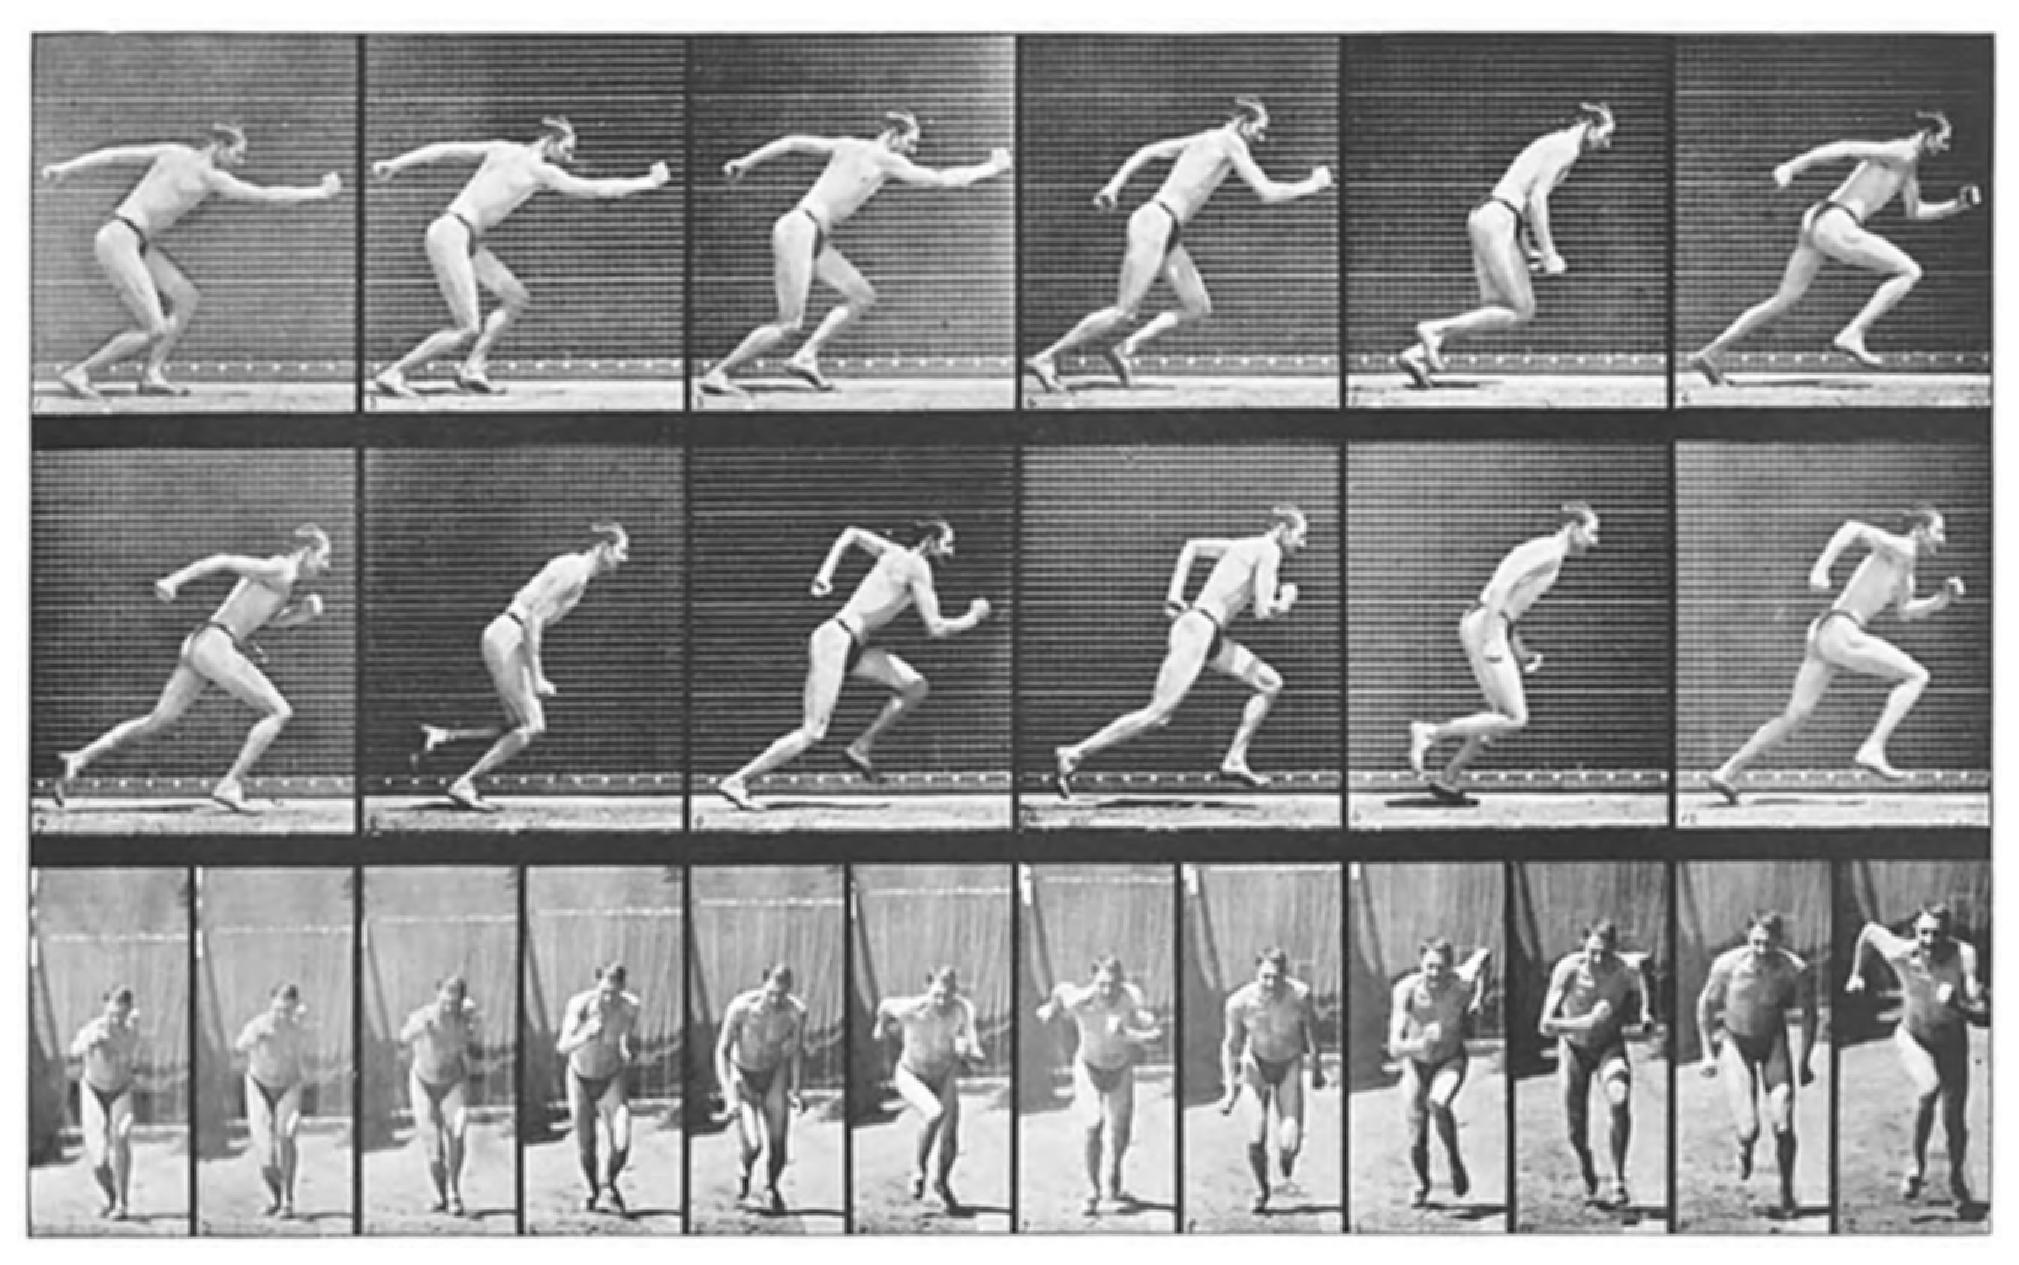
\includegraphics[width=15cm]{figuras/inicio_corrida.eps}
	\caption{Atleta iniciando uma corrida. Fonte: \citeonline{Muybridge1885}.}
	\label{inicio_corrida}
\end{figure}


Apesar dos avanços ocorridos na análise de marcha até meados do meio do século vinte, foi só após o advento dos computadores modernos que a análise de marcha clínica tornou-se amplamente disponível \cite{Baker2007}.



\subsection{FUNDAMENTOS}
Segundo \citeonline{Perry2010}, para se classificar as diferentes divisões da marcha é necessário separá-las em períodos, fases e tarefas, conforme a Figura \ref{fases_marcha}.

\begin{figure}[ht]
	\centering
	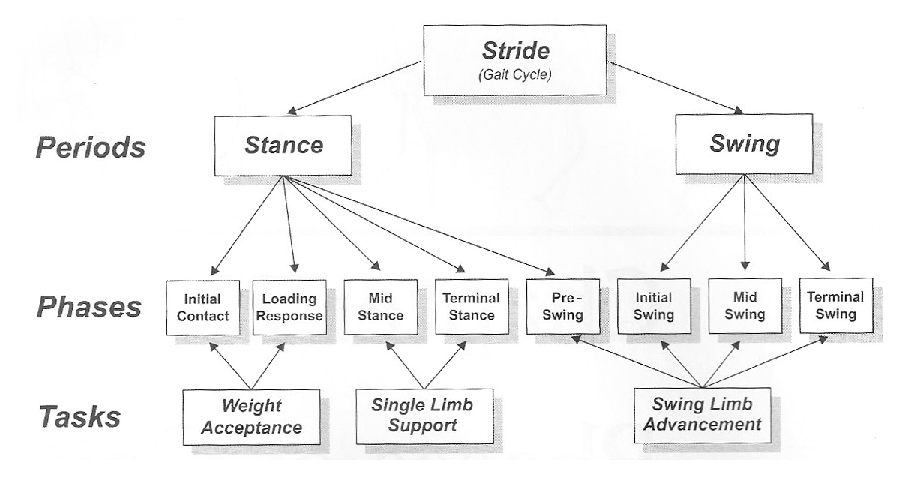
\includegraphics[width=15cm]{figuras/fases_marcha.eps}
	\caption{Divisões do Ciclo de Marcha. Fonte: \citeonline{Perry2010}.}
	\label{fases_marcha}
\end{figure}

A passada, que também é um sinônimo para um ciclo de marcha completo, equivale ao momento que, por exemplo, o pé direito toca o chão, sai do chão e o toca novamente. Dentro do ciclo de marcha temos também os períodos que são dois, apoio e balanço. 
O apoio corresponde ao período que o pé toca o chão pela primeira vez e o deixa durante o ciclo. 
O balanço é o período que o mesmo pé deixa o chão e o toca novamente iniciando um novo apoio \cite{Perry2010}. 

Além dos períodos, como vemos na Figura \ref{fases_marcha}, temos as fases. As fases representa um intervalo, percentual durante o ciclo da marcha e são muito importantes na avaliação do ciclo, 
pois grandes variações nos sinais durante alguma fase, pode representar algum distúrbio a ser diagnosticado. São oito as fases \cite{Perry2010}:
\begin{enumerate}
	\item Contato inicial, corresponde de 0 a 2\% do ciclo de marcha;
	\item Resposta à carga, corresponde de 2\% até 12\% do ciclo de marcha;
	\item Apoio médio, corresponde de 12\% até 31\% do ciclo de marcha;
	\item Apoio terminal, corresponde de 31\% até 50\% do ciclo de marcha;
	\item Pré-balanço, corresponde de 50\% ate 62\% do ciclo de marcha;
	\item Balanço inicial corresponde de 62\% até 75\% do ciclo de marcha;
	\item Balanço médio corresponde de 75\% até 87\% do ciclo de marcha;
	\item Balanço terminal corresponde de 87\% até 100\% do ciclo de marcha. 
\end{enumerate}

As tarefas são as funções desempenhadas durante o ciclo de marcha e estão relacionadas especificamente com as fases. 
A Figura \ref{fases_marcha} mostra o relacionamento entre as três tarefas e suas fases específicas. São elas \cite{Perry2010}:
\begin{enumerate}
	\item \emph{Aceitação de Peso} - Ela é responsável pela absorção do choque, estabilidade inicial de membro e preservação da progressão;
	\item \emph{Apoio Simples} - Esta tarefa é responsável por manter um membro apoiado no chão e progredindo o ciclo de marcha, até que o outro membro toque o chão, ou seja, sua função, é fazer que um membro suporte todo o peso do corpo sozinho;
	\item \emph{Avanço do Membro} - Sua função é avançar o membro que está no período de balanço, até que ele esteja pronto para fazer um novo contato inicial.
\end{enumerate}

\subsection{MÉTODOS DE COLETA DE DADOS PARA ANÁLISE} 
\label{metodos_analise}

Esta seção descreve alguns dos dispositivos que podem ser usados para coletar dados de movimentos. 
Estes podem ser convertidos e usados pelo software desenvolvido, desde que uma adaptação seja feita. 
No momento de conclusão deste trabalho o único método adaptado é o por captura de dados por câmeras, usando o sistema da \emph{Qualisys}.

\textbf{Captura de dados por câmeras}

\noindent
Pode-se começar este assunto pelos métodos de mensuração de movimentos espaciais e de ângulos.
O método mais sofisticado hoje para análise de movimentos é o baseado em câmaras de vídeo. 
Inclusive \citeonline{Grip2013}, demonstra discorre sobre as vantagens dos sistemas de câmeras ópticas usando marcadores de superfície em detrimento de outras técnicas de captura de movimento. 
Neste tipo de técnica, os marcadores podem ser ativos ou passivos, a diferença é que os ativos emitem algum tipo de sinal luminoso ou infravermelho, por exemplo. 
Este método permite visualizar a posição espacial dos marcadores e a partir daí, calcular velocidades, acelerações, ângulos, velocidades angulares, acelerações angulares, etc.
A Figura \ref{oqus_mri} mostra o modelo \emph{Oqus MRI} da \emph{Qualisys}. Esta é uma câmera muito utilizada no mercado não só para análise clínica mas também para captura de movimentos para serem inseridos em filmes e jogos de computador. 
Já a Figura \ref{visao_qtm} mostra o software QTM do mesmo fabricante, já com os dados capturados e animados na tela do computador.
A Figura \ref{markers} é uma visão de uma possível configuração de câmeras, capturando marcadores de superfície passivos de um paciente.

\begin{figure}[H]
	\centering
	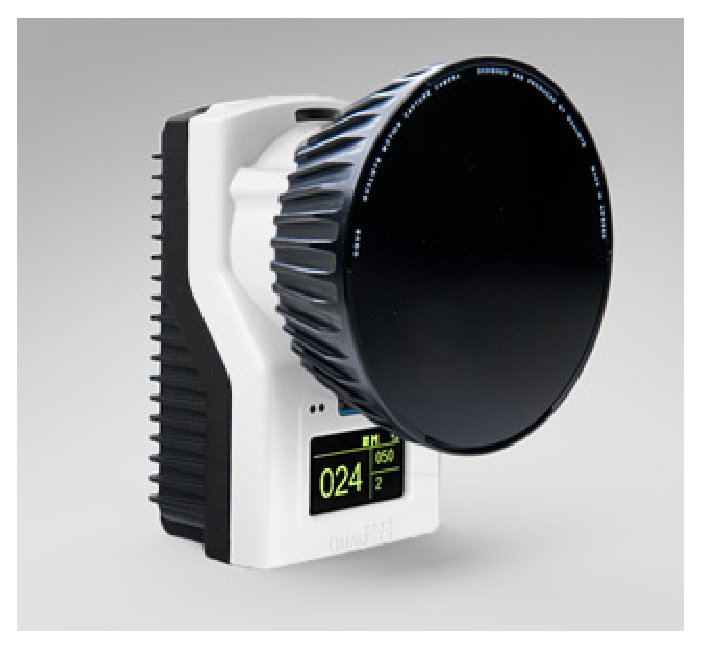
\includegraphics[width=7cm]{figuras/oqus-mri.eps}
	\caption{Câmera Oqus MRI. Fonte: \citeonline{Qualisys2013}.
}
	\label{oqus_mri}
\end{figure}


\begin{figure}[H]
	\centering
	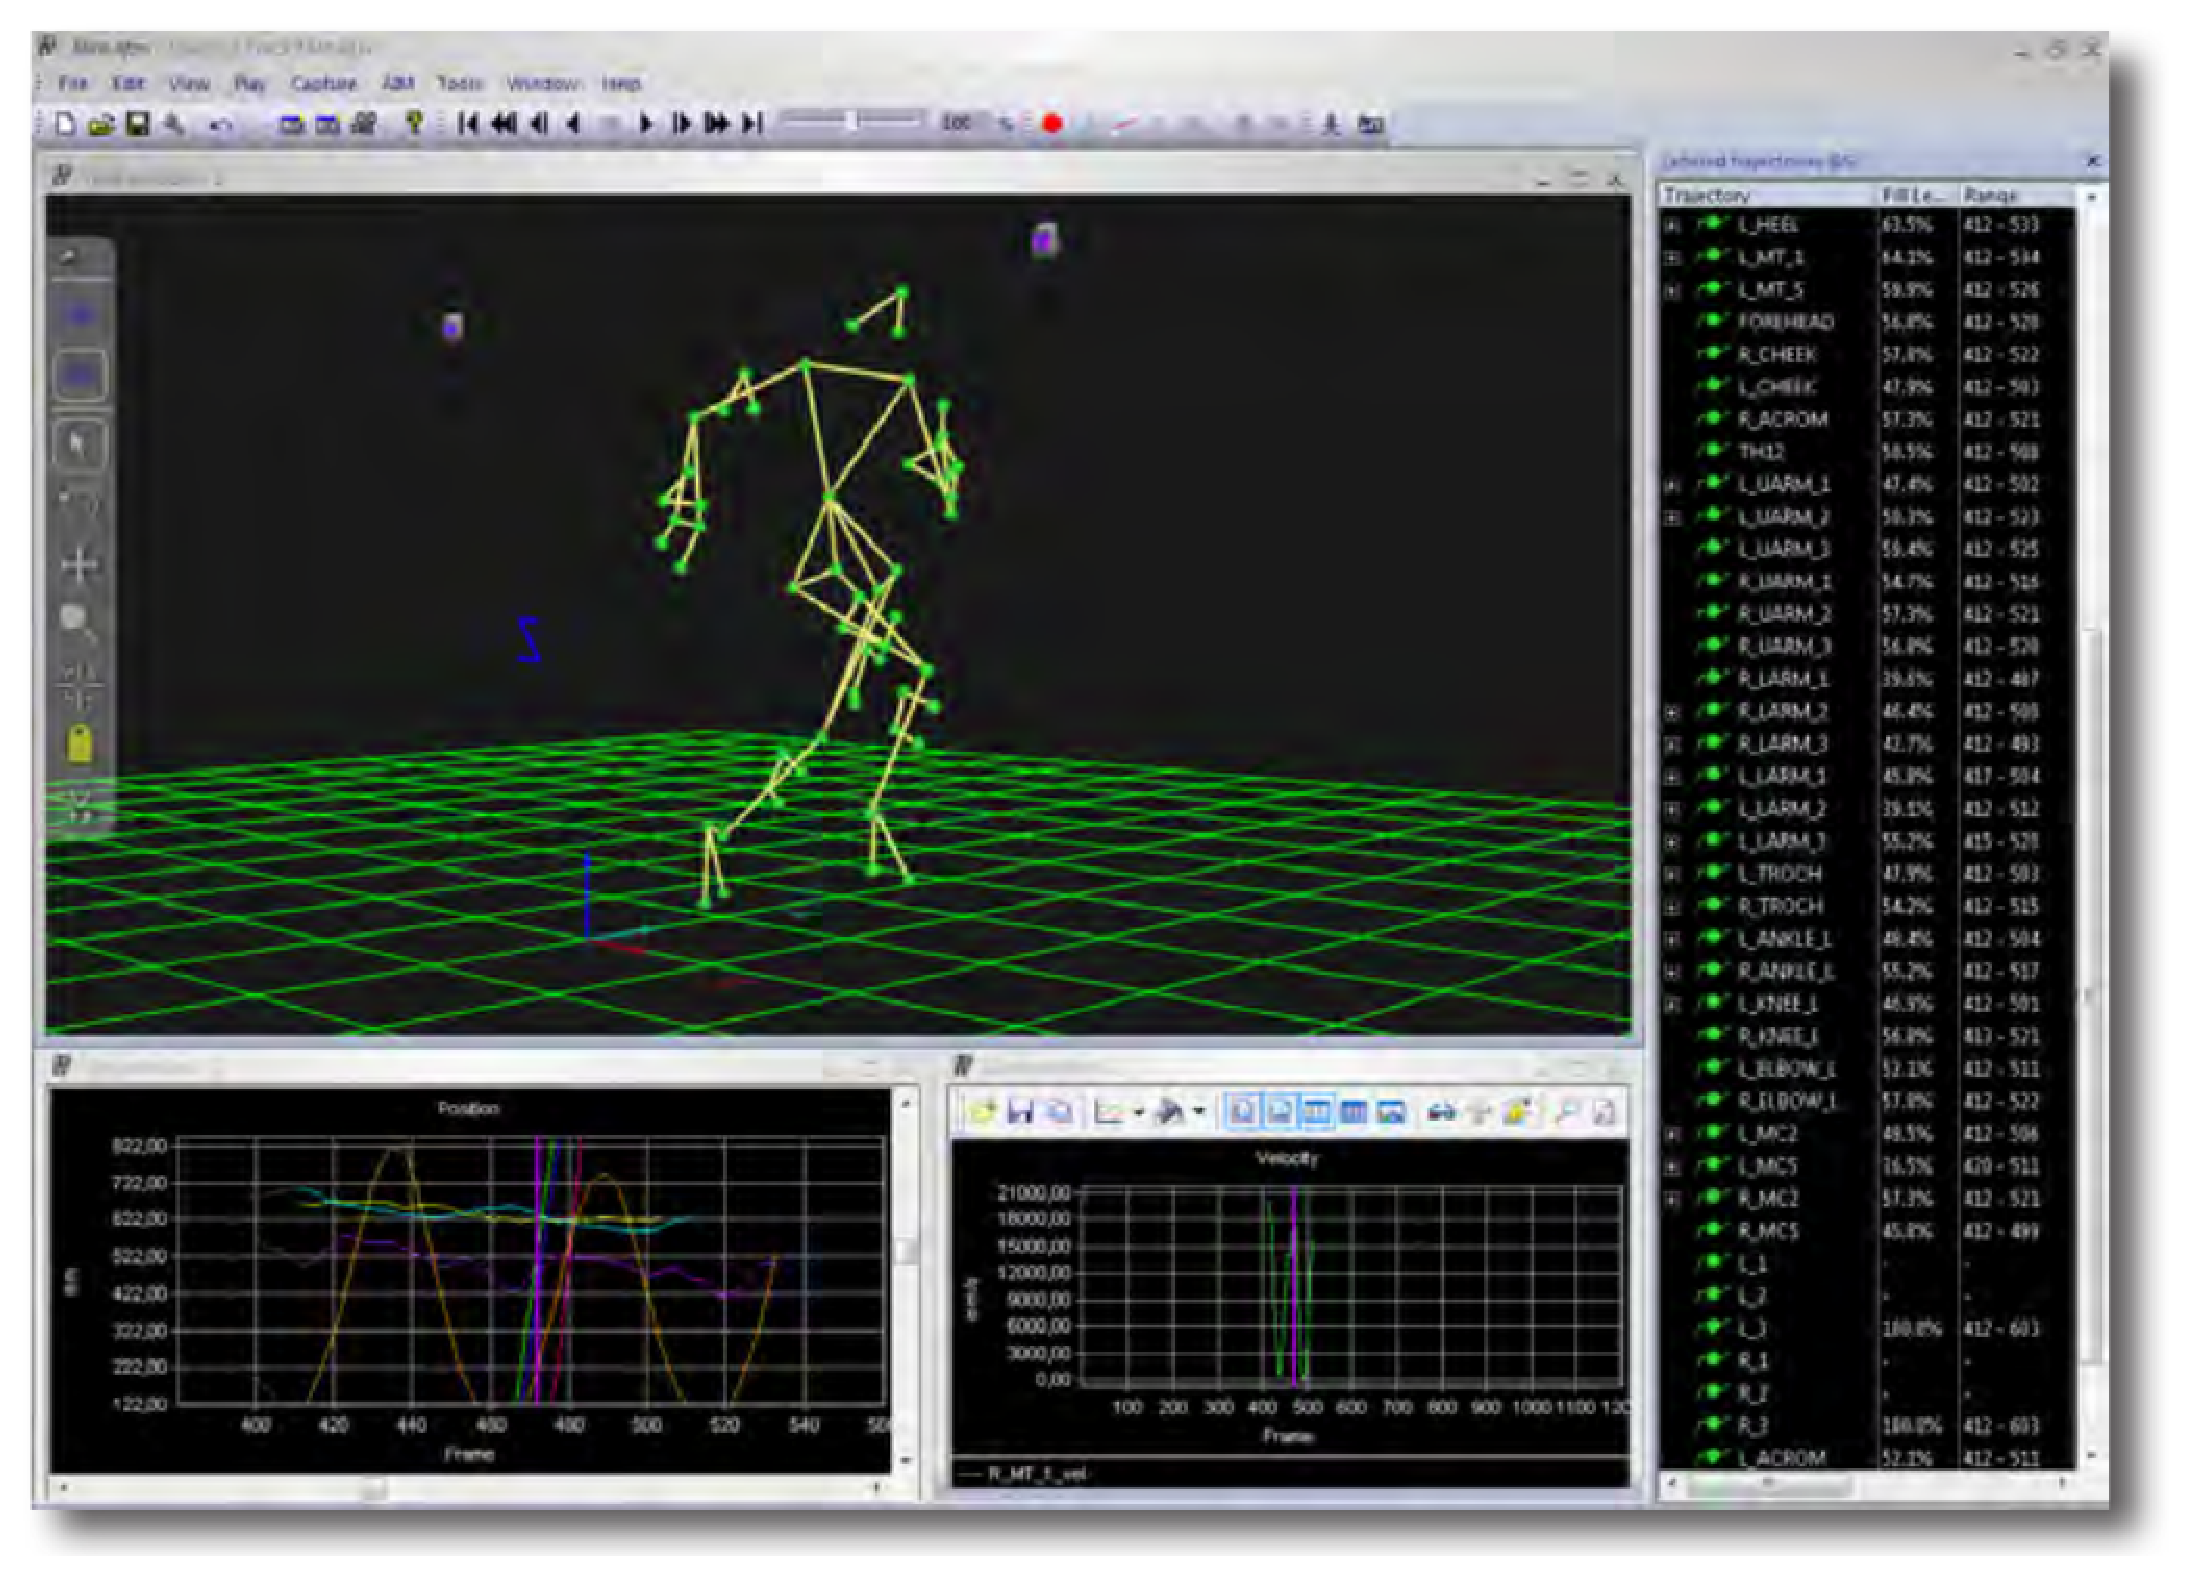
\includegraphics[width=15cm]{figuras/qtm.eps}
	\caption{Visão do QTM. Fonte: \citeonline{Qualisys2010}.}
	\label{visao_qtm}
	
\end{figure}


\begin{figure}[H]
	\centering
	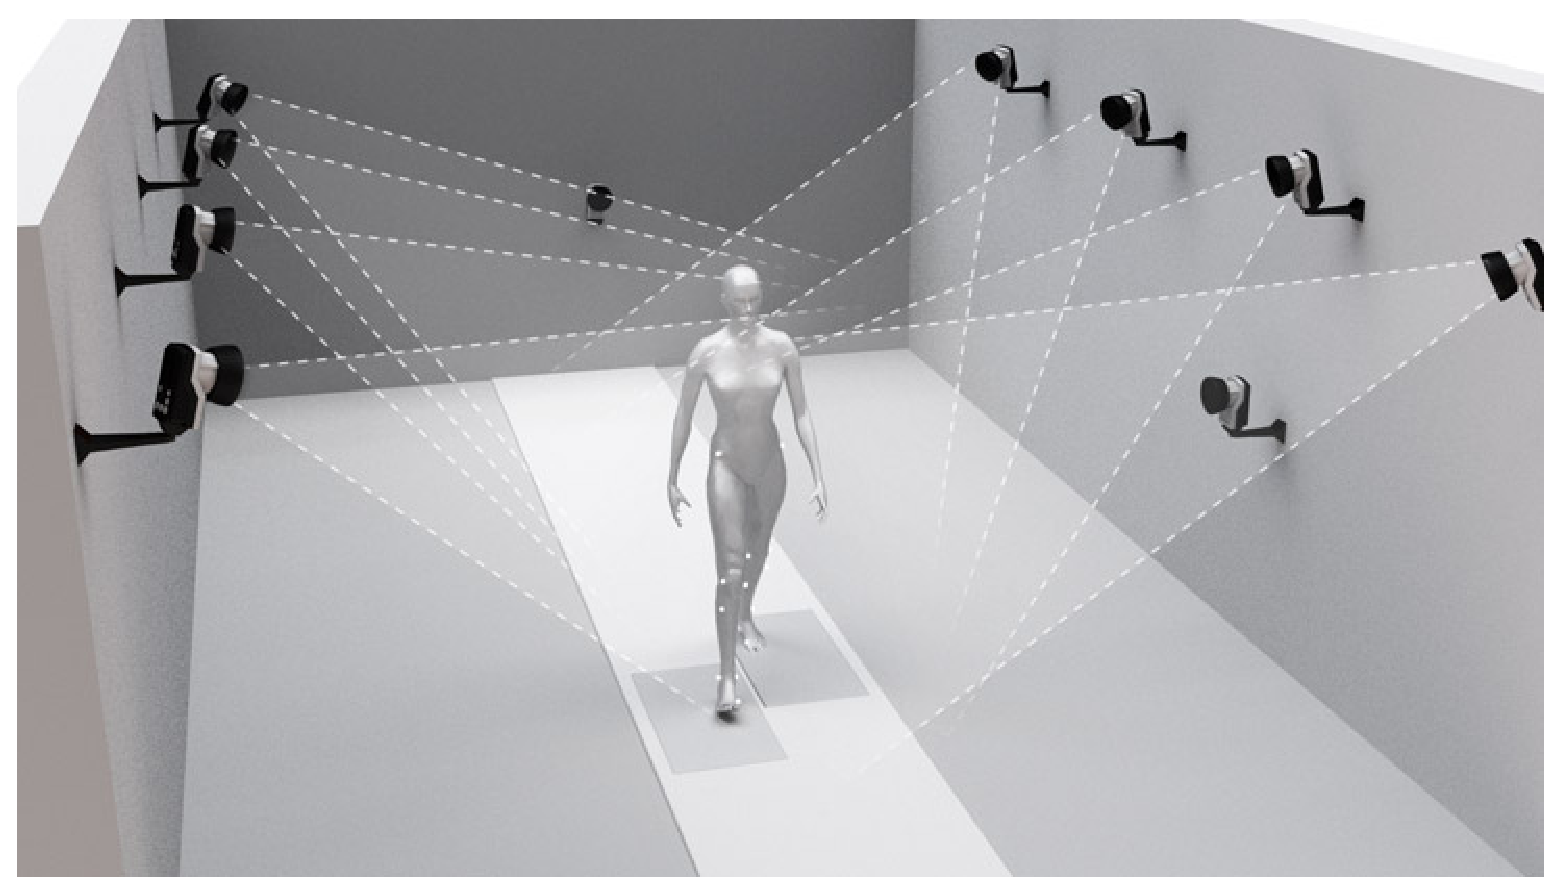
\includegraphics[width=14cm]{figuras/markers.eps}
	\caption{Configuração de câmeras para captura de dados de marcadores passivos fixados no paciente. Fonte: \citeonline{Qualisys2013a}.}
	\label{markers}
	
\end{figure}


\textbf{Captura por Unidade de Medida Inercial}

\noindent
Uma outra alternativa, que está sendo desenvolvida na FGA/UnB, é um dispositivo baseado em uma Unidade de Medida Inercial \emph{(Inertial Measurement Unit - IMU)}. O IMU é um dispositivo eletrônico provido de acelerômetrose um magnetômetro.
Segundo \citeonline{Leite2014}, esta é uma alternativa não visual para extrair parâmetros cinemáticos da marcha humana, trajetória e velocidade. 
O trabalho foi realizado comparando-se os resultados fornecidos pelo dispositivo e captura de vídeo.
A Figura \ref{imu} mostra um experimento onde o vídeo e os dados do \emph{IMU} são coletados ao mesmo tempo.


Na Figura \ref{imu2}, é possível visualizar o resultado dos dados coletados do \emph{IMU} e da câmera. 
Veja que é um resultado bem promissor. 
Mas a maior vantagem do dispositivo, ainda não foi discutida, seu baixíssimo valor em relação a solução com várias câmeras.

\begin{figure}[H]
	\centering
	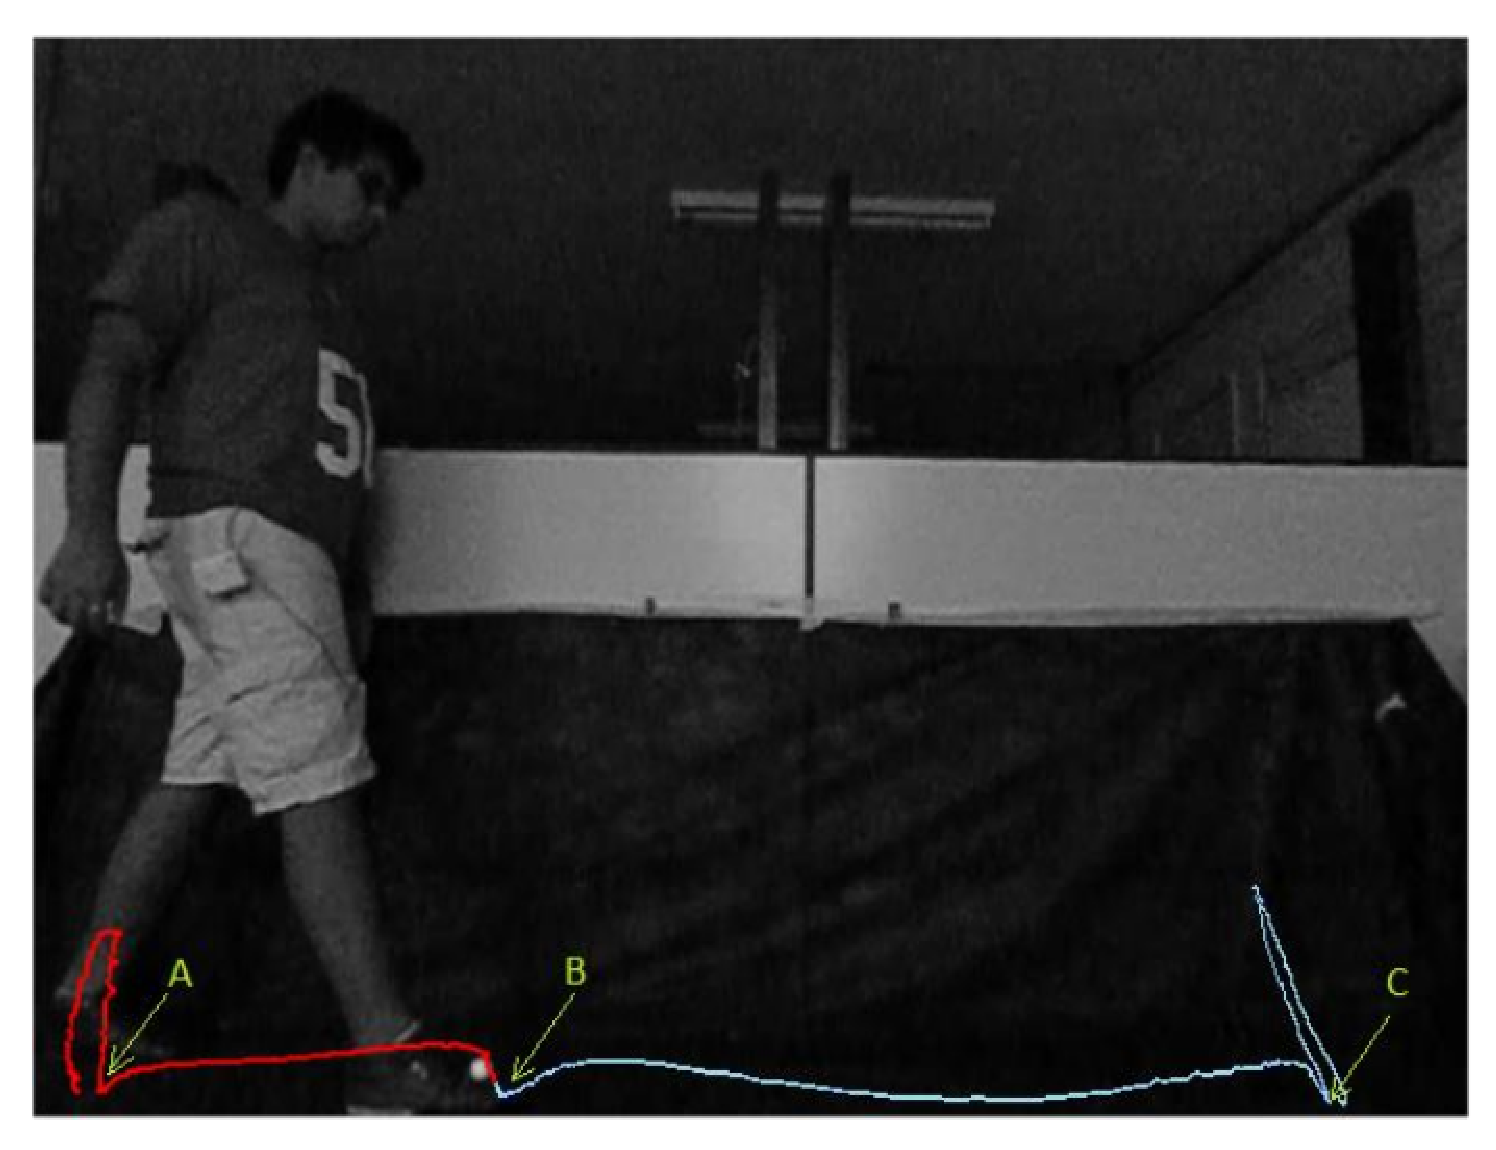
\includegraphics[width=7cm]{figuras/imu.eps}
	\caption{Experimento de captura de dados de \emph{IMU} em conjunto com uma câmera. Fonte: \citeonline{Leite2014}.}
	\label{imu}
	
\end{figure}


\begin{figure}[H]
	\centering
	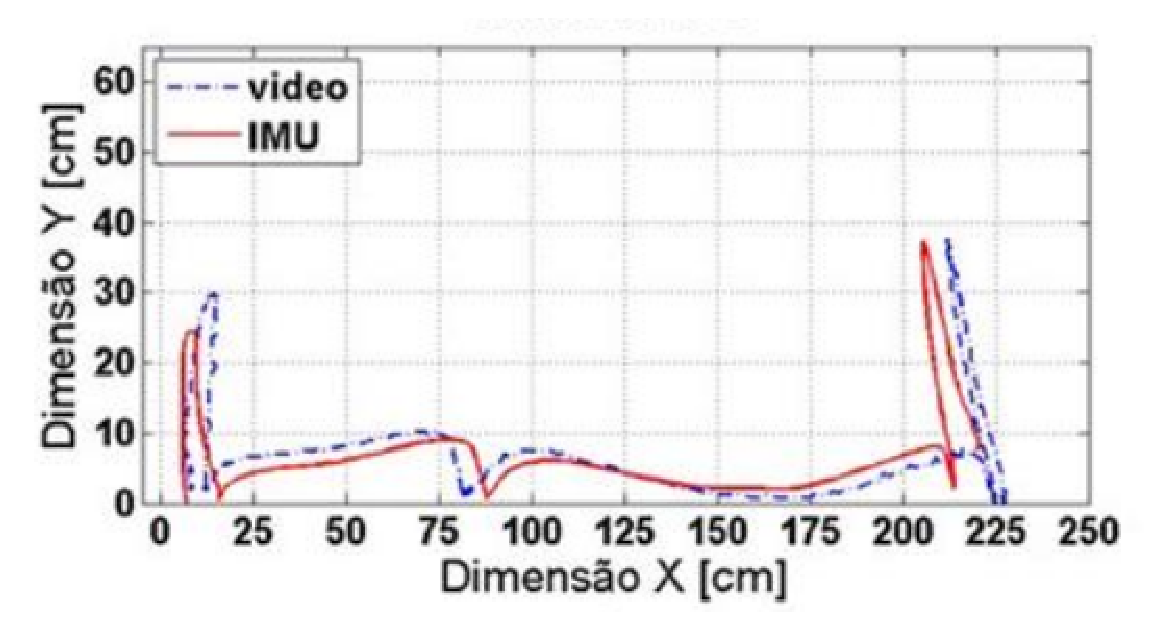
\includegraphics[width=10cm]{figuras/imu2.eps}
	\caption{Comparação entre \emph{IMU} e a câmera. Fonte: \citeonline{Leite2014}.}
	\label{imu2}
	
\end{figure}



\textbf{Captura por Eletrogoniômetros}

\noindent
Eletrogoniômetros são também usados para capturar angulações em articulações, basicamente este aparelho provê uma voltagem que é representativa da mudança de ângulo entre duas superfícies, nas quais o dispositivo é fixado \cite{K.Ibrahim2012}. 
A principal vantagem deste dispositivo é que seu custo é baixo. A Figura \ref{egn} mostra um exemplo de eletrogoniômetro.
Ele tem como desevantagem sua pouca precisão, mas ainda assim pode ser usado na análise de movimentos por software.



\begin{figure}[H]
	\centering
	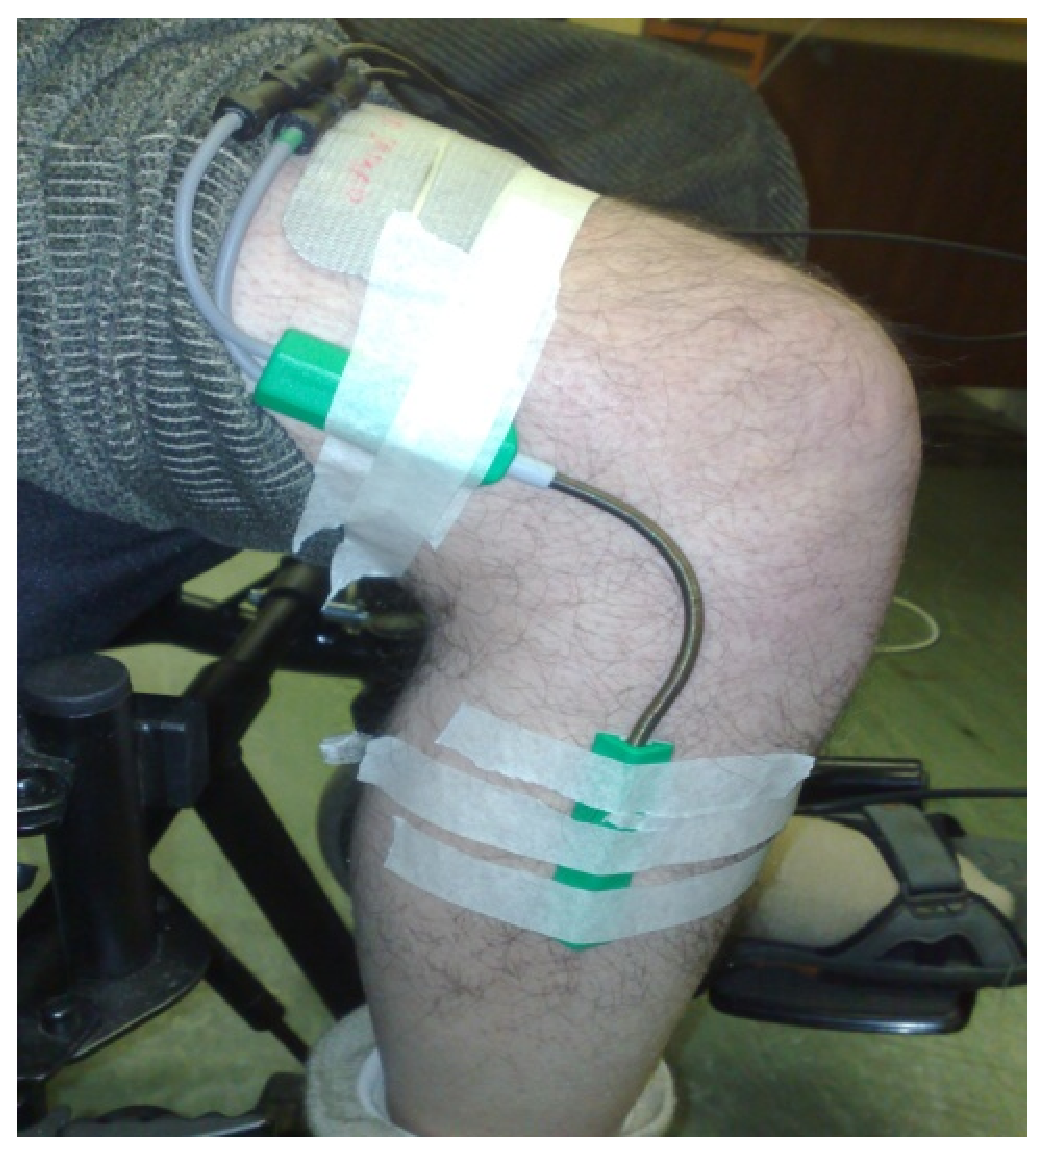
\includegraphics[width=7cm]{figuras/egn.eps}
	\caption{Eletrogoniômetro. Fonte: \citeonline{K.Ibrahim2012}.}
	\label{egn}
	
\end{figure}




\section{MÉTODOS ÁGEIS}
A muito tempo vários métodos para desenvolvimento de software são propostos. 
Em 2001, um grupo de pessoas muito experientes em desenvolvimento de software, juntaram-se em Salt Lake City, Utah, para resolverem problemas de desenvolvimento de software \cite{Greene2014}.
Como resultado deste encontro, foi criado o manifesto ágil, que é reproduzido a seguir \cite{Beck2001}:

\begin{citacao}

Estamos descobrindo maneiras melhores de desenvolver software, fazendo-o nós mesmos e ajudando outros a fazerem o mesmo. 
Através deste trabalho, passamos a valorizar:

Indivíduos e interações mais que processos e ferramentas;

Software em funcionamento mais que documentação abrangente;

Colaboração com o cliente mais que negociação de contratos;

Responder a mudanças mais que seguir um plano.

Ou seja, mesmo havendo valor nos itens à direita, valorizamos mais os itens à esquerda.
\end{citacao}

Meses após a criação do manifesto, estas pessoas também criaram os princípios ágeis e a Aliança Ágil \cite{Layton2012}.

Os princípios ágeis são um conjunto de 12 itens com o objetivo de auxiliar na implantação de metodologias ágeis. Eles são reproduzidos a seguir a título de ilustração \cite{Beck2001}:

\begin{citacao}
		1. Nossa maior prioridade é satisfazer o cliente
		através da entrega contínua e adiantada
		de software com valor agregado.

		2. Mudanças nos requisitos são bem-vindas,
		mesmo tardiamente no desenvolvimento.
		Processos ágeis tiram vantagem das
		mudanças visando vantagem competitiva para o cliente.

		3. Entregar frequentemente software funcionando,
		de poucas semanas a poucos meses,
		com preferência à menor escala de tempo.

		4. Pessoas de negócio e desenvolvedores devem trabalhar
		diariamente em conjunto por todo o projeto.

		5. Construa projetos em torno de indivíduos motivados.
		Dê a eles o ambiente e o suporte necessário
		e confie neles para fazer o trabalho.

		6. O método mais eficiente e eficaz de transmitir
		informações para e entre uma equipe de desenvolvimento
		é através de conversa face a face.

		7. Software funcionando é a medida primária de progresso.

		8. Os processos ágeis promovem desenvolvimento
		sustentável. Os patrocinadores, desenvolvedores e
		usuários devem ser capazes de manter um ritmo
		constante indefinidamente.

		9. Contínua atenção à excelência técnica e bom design
		aumenta a agilidade.

		10. Simplicidade--a arte de maximizar a quantidade de
		trabalho não realizado--é essencial.

		11. As melhores arquiteturas, requisitos e designs
		emergem de equipes auto-organizáveis.

		12. Em intervalos regulares, a equipe reflete sobre como
		se tornar mais eficaz e então refina e ajusta seu
		comportamento de acordo. 
\end{citacao}

Este manifesto serviu de marco agregador de métodos e técnicas, que já existiam a época, mas não eram amplamente difundidas como \emph{Scrum}, \emph{Extreme Programming}, \emph{kanban}, \emph{lean}, entre outros. 
Estas técnicas, apesar de anteriores ao manifesto, possuem em seus cernes, muito em comum com os valores ágeis.
A Figura \ref{cap2_valores} tenta ilustrar esta ideia.

\begin{figure}[H]
	\centering
	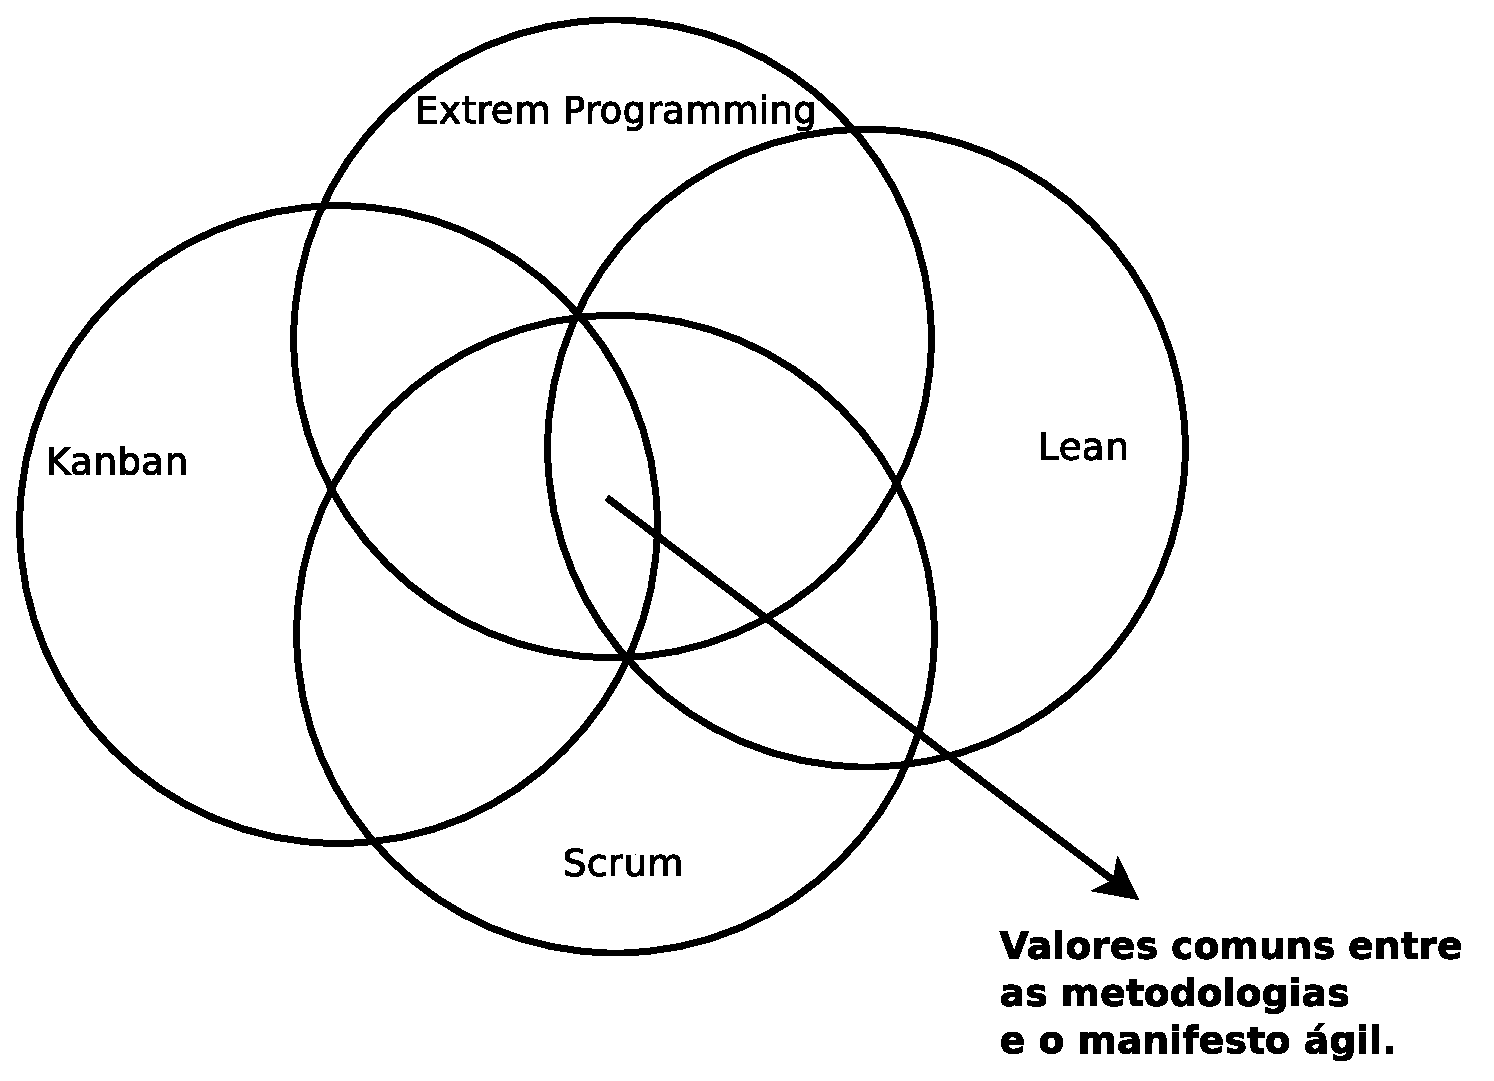
\includegraphics[width=7cm]{figuras/cap2_valores.eps}
	\caption{Valores em comum. Fonte: Alterado de \citeonline{Greene2014}.}
	\label{cap2_valores}
\end{figure}

A adoção dos métodos ágeis hoje é praticamente unanimidade. 
Isto se deve aos modelos de desenvolvimento adotados até a década de 1990. 
Esses modelos eram na sua grande maioria baseados no modelo \emph{waterfall}, que imitava uma linha de produção onde o software era desenvolvido em fases. 
A saída de cada fase era a entrada da próxima. 
A Figura \ref{waterfall} mostra um exemplo de processo baseado no modelo \emph{waterfall}.
O maior problema do modelo \emph{waterfall}, era que este foi completamente averso a mudanças de requisitos. 
Hoje, é notório que a grande maioria dos softwares necessitam ser bastante receptivos a mudanças.

O trabalho de \citeonline{KristinRunyan2014} compara o modelo \emph{waterfall} com o modelo ágil. 
Esta comparação é resumidamente apresentada na Tabela \ref{waterfall_x_agil}.

\begin{table}[H]
	\caption{Comparando Modelos de Desenvolvimento de Software}
	\label{waterfall_x_agil}
	\ABNTEXfontereduzida
	\begin{tabular}{p{8cm}p{8cm}}
	\toprule
	\textit{Waterfall} & \textit{Ágil}\\
	\midrule
	\ABNTEXfontereduzida
	Prescritivo & Abstrato\\
	Documentação extensiva & Mínimo de documentação\\
	Sequencial & Contínuo\\
	Formal & Informal\\
	Foco no processo & Foco na comunicação\\
	Mudança gradual & Mudança rápida\\
	\bottomrule
	\end{tabular}
	\footnotesize Fonte:
	\citeonline{KristinRunyan2014}
\end{table}

Como evolução do modelo \emph{waterfall}, surgiram os processos baseados em modelos iterativos. 
A diferença agora é que o processo de desenvolvimento passa a ser baseado em ciclos. 
Cada ciclo passa por cada uma das fases do \emph{waterfall}. 
Este tipo de processo, apresentava melhoras, mas ainda era concebido sob a forma de um processo que visava resolver problemas determinísticos, como o das linhas de produção das fábricas.
Mas, como descrito em \citeonline{Beck2004}, o processo de se construir software é mais parecido com o ato de dirigir.
O motorista sabe o destino a que quer chegar, porém, durante o percurso pode haver um acidente e tem-se que mudar um pouco a rota, ou alguém está passando por uma faixa de pedestre e necessita-se parar, ou ainda um sinal de transito pode ficar vermelho. 
Esta é a principal motivação para que este trabalho privilegie métodos ágeis de desenvolvimento.


\begin{figure}[H]
	\centering
	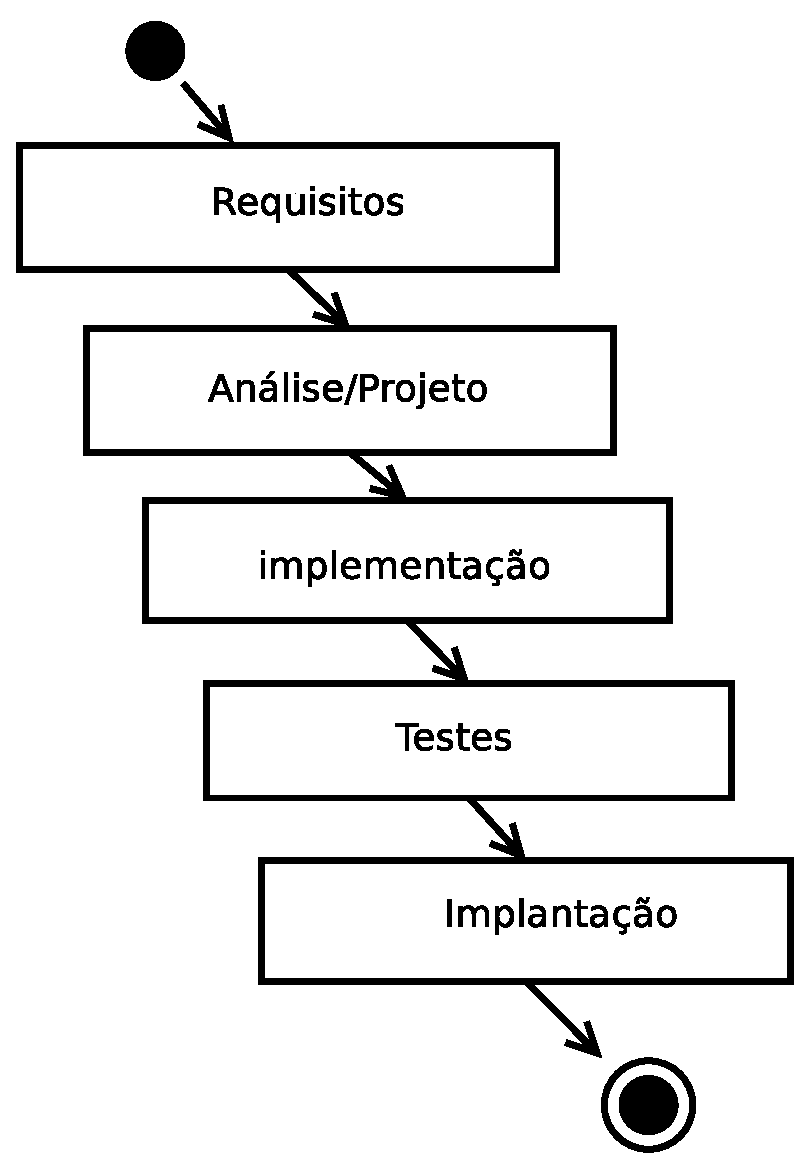
\includegraphics[width=4cm]{figuras/waterfall.eps}
	\caption{Exemplo de processo baseado no modelo \emph{waterfall}. Fonte: Alterado de \citeonline{Pressman2014}.}
	\label{waterfall}
\end{figure}



\subsection{SCRUM}
\label{scrum_sec}

O \emph{Scrum}, segundo \citeonline{Rubin2012}, é um método ágil para desenvolvimento de produtos e serviços inovadores. 
A Figura \ref{scrum_geral} mostra uma visão geral do \emph{Scrum}.


Basicamente, o fluxo do scrum consiste na criação de um \emph{backlog} de produto. 
Este \emph{backlog} é uma lista de requisitos a serem implementados no processo de desenvolvimento, e é mantido e priorizado pelo \emph{product owner}. 
A lista em si pode receber contribuições dos mais diversos envolvidos no processo, mas a última palavra na priorização é sempre do \emph{product owner}.
A orientação mais aceita para a priorização dos requisitos, é levar em conta aqueles que mais gerarão valor para o usuário final, no momento em questão \cite{Schwaber2001}.

A próxima etapa no fluxo é a reunião de \emph{sprint}. 
Esta reunião consiste na demonstração das funcionalidades implementadas na última iteração e na seleção das funcionalidades que serão construídas na próxima iteração.
As funcionalidades são escolhidas pelos desenvolvedores, que se comprometem a entregá-las ao final da iteração \cite{Schwaber2004}.


\begin{figure}[H]
	\centering
	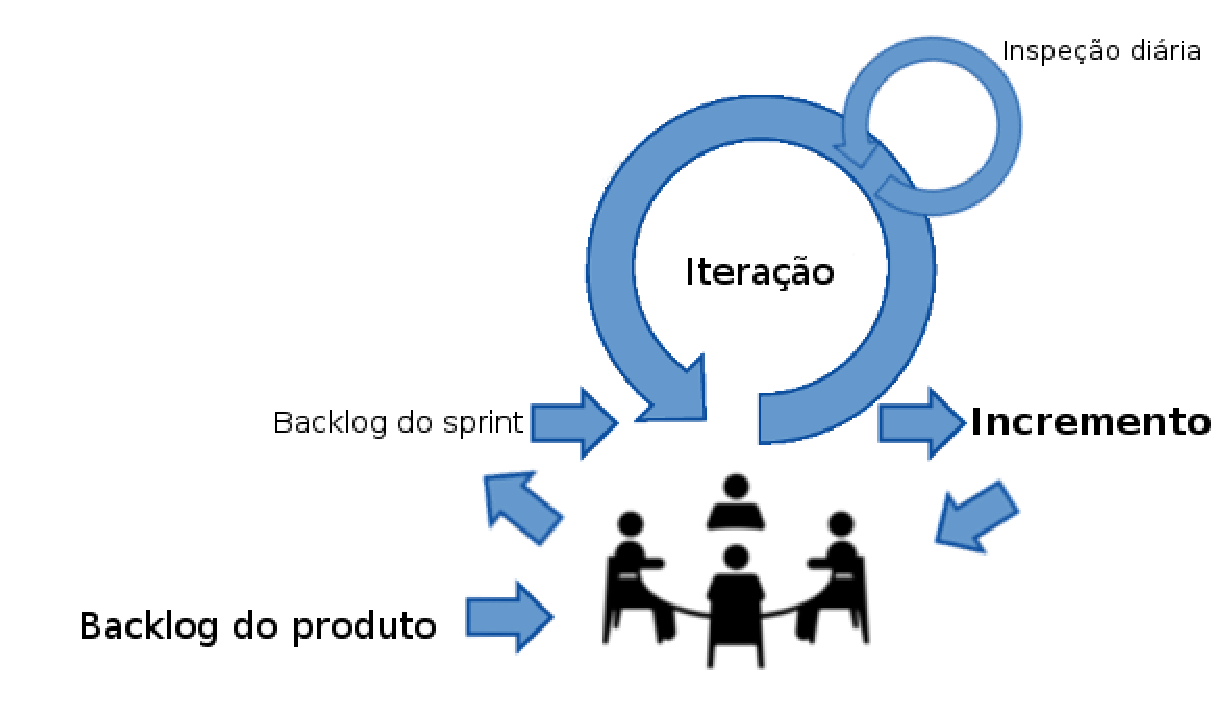
\includegraphics[width=15cm]{figuras/scrum_geral.eps}
	\caption{Visão Geral do \emph{Scrum}. Fonte: Alterado de \citeonline{Schwaber2004}.}
	\label{scrum_geral}
\end{figure}



Após a reunião do \emph{sprint}, inicia-se a iteração. A iteração é também chamada de \emph{sprint} e consiste num prazo de alguns dias ou alguns meses. 
Isto depende do projeto em questão. Geralmente \emph{sprints} menores são mais aconselhados, por exemplo, uma semana  \cite{Schwaber2004}.

Durante a iteração ou \emph{sprint}, ao final do dia preferencialmente, realiza-se uma reunião de inspeção diária. 
Esta reunião é também chamada de \emph{daily scrum}. 
Nesta reunião, os envolvidos diretamente no desenvolvimento do produto ou serviço, expõe o andamento de suas atividades pessoais e os impedimentos para a conclusão destas. 
A reunião é feita com todos de pé, e cada um dispõe apenas de alguns minutos de exposição, por exemplo, 3 minutos. 
A intromissão de pessoas externas deve ser evitada. 
A ideia é manter a objetividade e o foco nas tarefas do \emph{sprint}.
Ao final da reunião o \emph{scrum master} deve procurar intender todos os impedimentos expostos. A partir deste conhecimento ele deve tomar medidas necessárias para removê-los, assim garantindo o bom funcionamento da equipe de desenvolvimento.
Ao final do \emph{sprint} um incremento, ou seja, um pedaço de software com funcionalidades implementadas é construído e preferencialmente implantado. O próximo passo é uma nova reunião de \emph{sprint}.

Os papéis definidos pelo \emph{scrum} são \cite{Schwaber2004}:
\begin{itemize}	
	\item \emph{Product Owner};
	\item \emph{Scrum Master};
	\item Desenvolvedor.
\end{itemize}

Nas organizações existirão outros papeis, como gerentes, diretores, patrocinadores, usuários finais, entre outros. 
O importante a se observar, é que apenas os três papeis, \emph{product owner}, \emph{scrum master} e desenvolvedor, é que fazem parte da equipe \emph{scrum}. 
Os demais papeis participam do projeto, mas é necessário, o entendimento por parte da organização, que demandas de implementação devem ser colocadas no backlog do produto. 
Só o \emph{product owner} pode priorizar os novos requisitos. 
Sem este entendimento e comprometimento, fica inviável respeitar prazos e escopo, tornando o processo caótico \cite{Schwaber2004}.

Devido ao \emph{Scrum} servir de espinha dorsal a um processo de desenvolvimento ágil, também sendo amplamente utilizado pelo mercado de desenvolvimento de software, ele foi selecionado como método de gestão deste trabalho. 
Todo o processo do \emph{Scrum} pode ser minunciosamente estudado em \citeonline{Schwaber2001}.


\subsection{HISTÓRIAS DO USUÁRIO}
\label{user_stories_sec}

Histórias do usuário é uma técnica que vem em detrimento da produção massiva de requisitos. 
Até hoje é comum achar projetos de desenvolvimento de software, com documentos de requisitos enormes. 
Com raras exceções, este não é um modelo muito produtivo. 
O grande problema é que muitas vezes gasta-se muito tempo, às vezes anos, para se criar estes documentos. 
Enquanto isso pouco ou nada de software funcional é produzido. 
Uma consequência comum desta demora, são as prioridades dos usuários mudarem, ou seja, o que foi especificado inicialmente, depois de um ano, por exemplo, já não tem o mesmo valor para os mesmos \cite{Patton2014}.

De acordo com \citeonline{cohn2004} histórias do usuário descrevem funcionalidades que serão de valor para um usuário ou comprador de um sistema de software. Histórias do usuário são compostas por três aspectos: 
\begin{itemize}
	\item Uma descrição escrita da história usada para planejamento e como lembrete;
	\item Conversações sobre a história para detalhar a mesma;
	\item Testes que trazem e documentam detalhes e que podem ser usadas para determinar quando a história está completa.
\end{itemize}

Histórias do usuário podem ser documentadas usando-se \emph{story cards}. Um exemplo é mostrado na Figura \ref{story_card}.

No \emph{story card} em questão, a parte superior é a descrição do item que é de valor para um usuário. 
A parte inferior relata testes que devem ser executados. 
Estes testes também servem para determinar se a história do usuário foi completamente implementada ou não \cite{cohn2004}.

Dentro de uma metodologia como o \emph{Scrum}, as histórias de usuário podem ser utilizadas para comporem o \emph{backlog} do produto. 
Elas são excelentes durante a fase de planejamento do \emph{sprint} \cite{Hanley2015}. 

Como as histórias do usuário são documentos mais informais, é necessário que as mesmas sejam mais detalhadas durante o processo de desenvolvimento. 
Isto pode ser feito com uma conversa entre o desenvolvedor e o \emph{product owner}. 
Pode se chegar a conclusão que a história é na verdade um "épico", ou seja, é uma história composta de outras histórias. 
Neste caso a história dever ser quebrada e suas partes enviadas para planejamento novamente \cite{cohn2004}. 

\begin{figure}[ht]
	\centering
	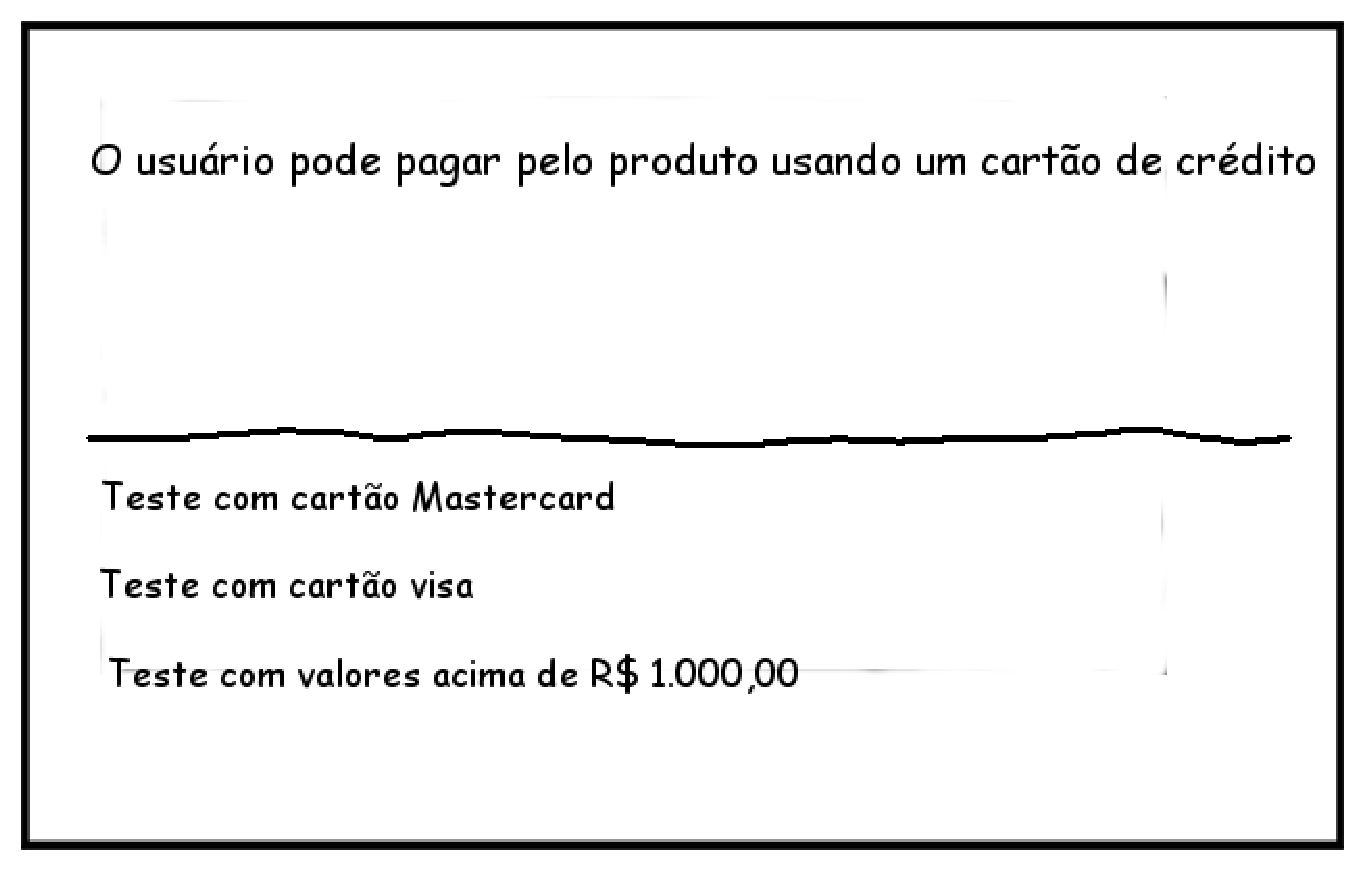
\includegraphics[width=15 cm]{figuras/story_card.eps}
	\caption{Exemplo de \emph{story card}. Fonte: Alterado de \citeonline{cohn2004}.}
    	\label{story_card}
\end{figure}




\section{SOFTWARE COMO SERVIÇO} 

A ideia de software como serviço é bastante difundida atualmente. 
Redes sociais, serviços de busca, serviços de \emph{streaming} de vídeo, são amplamente usados por todos. 
Segundo \citeonline{Fox2012} software como serviço, é definido como o software que entrega software e dados como serviços sobre a \emph{Internet}, usualmente via um programa como um \emph{browser} que roda num dispositivo cliente local, em detrimento de código binário que precisa ser instalado e que roda totalmente no dispositivo.

Várias vantagens são citadas em \citeonline{Fox2012}, tanto para usuários quanto para desenvolvedores de software. São elas:

\begin{enumerate}
	\item Desde de que os usuários não necessitam instalar a aplicação, eles não precisam se preocupar se possuem um hardware específico, ou se possuem uma versão específica de sistema operacional;
	\item Como os dados associados ao serviço geralmente são mantidos com o serviço, os usuários não precisam fazer \emph{bakcups}, nem se preocupar em os perderem devido a mal funcionamento, ou até mesmo os perderem devido a extravios;
	\item Quando um grupo de usuários querem coletivamente interagir sobre os mesmos dados, software como serviço é um veículo natural;
	\item Faz mais sentido manter grandes quantidades de dados centralizados e manter o acesso remoto a estes;
	\item Os desenvolvedores podem controlar as versões de software e sistema operacional que executam o serviço. Isto evita problemas de compatibilidade com distribuição do software devido ao grande número de plataformas que os usuários possuem. Além disso, é possível que o desenvolvedor teste novas versões do software usando uma pequena fração dos usuários temporariamente, sem causar distúrbios na maioria dos usuários;
	\item Como os desenvolvedores controlam a versão de execução do software, eles podem mudar até mesmo a plataforma dos mesmos, desde que não violem as \emph{Aplication Program Interfaces (APIs)} de interface com o usuário.
\end{enumerate}

	Para quem duvida do poder do software como serviço, é só observar que produtos consagrado como o \emph{Microsoft Office} já possuem versão como serviço, no caso o \emph{Microsoft Office 365}. Outros exemplos seriam o \emph{Twitter}, \emph{Facebook}, entre outros.
	

Segundo \citeonline{Fox2012}, na visão de mais alto nível, de cima para baixo na figura \ref{saas_view}, vê-se o software como um site na \emph{web}. 
O cliente acessa o servidor via \emph{internet} usando um \emph{browser HTML}. 
Na segunda visão, vê-se uma aplicação \emph{web} em três camadas, apresentação, lógica e persistência.
A camada de apresentação serve páginas \emph{HTML} para o usuário. Estas páginas consomem a camada lógica, também conhecida como camada de negócios, que são responsáveis pela lógica de negócio da aplicação. Por último vem a camada de persistência responsável pelo armazenamento e recuperação dos dados da aplicação.
A próxima visão é uma extensão da segunda, nela detalha-se mais a camada lógica, que internamente funciona com uma arquitetura \emph{model-view-controller}. 
Basicamente esta arquitetura define entidades de negócio (\emph{model}), que são manipuladas por controladores (\emph{controller}) e preparadas para apresentação pelo mecanismo de apresentação (\emph{view}).
A última camada corresponde as tecnologias e padrões de projetos adotados pela aplicação em sim. Por exemplo, na figura seleciona-se o padrão de projeto \emph{active record} para implementação do \emph{model},  usando o estilo arquitetural \emph{REST} para implementação do \emph{controller} e o padrão de projeto \emph{template view} para a implementação do \emph{view}. Estas escolhas são dependentes de projeto e geralmente são feitas por um arquiteto de \emph{software} experiente. 

\begin{figure}[ht]
	\centering
	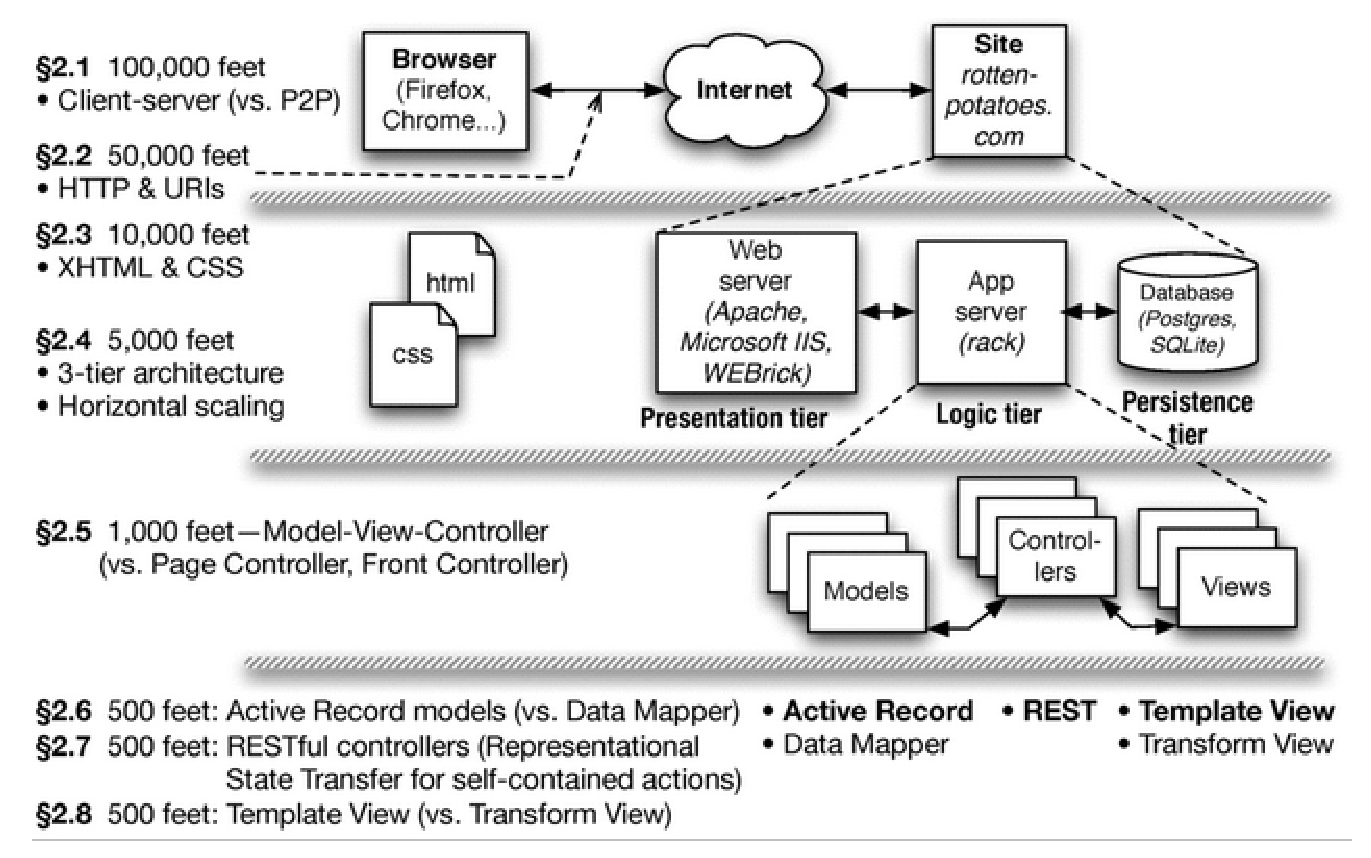
\includegraphics[width=15 cm]{figuras/saas_view.eps}
	\caption{Visões arquiteturais de software como serviço. Fonte: \citeonline{Fox2012}.}
    	\label{saas_view}
\end{figure}



\section[COMPONENTES, FRAMEWORKS E FERRAMENTAS]{COMPONENTES, \emph{FRAMEWORKS} E FERRAMENTAS}
Neste item serão analisados os components, \emph{frameworks} e ferramentas que foram selecionadas para construção do software. 
Este software será um serviço disponibilizado via \emph{web}, sendo assim, estas tecnologias são próprias para este fim. 

\subsection{APLICAÇÕES WEB COM \emph{ANGULAJS}}
\label{angularjs}
O \emph{AngularJS} é um \emph{framework} de aplicação \emph{web}. 
Ele foi projetado especificamente para rodar em \emph{browsers} que suportam \emph{HTML 5}.
Ele também é adequado a criação de aplicações \emph{web} que rodam em \emph{smartphones}. 
É um \emph{framework} bastante completo e rico para sua finalidade. 
A referência \citeonline{Branas2014} é um guia introdutório conciso no assunto.
 Segundo \citeonline{Freeman2014}, outro guia no assunto, o \emph{AngularJS} se baseia no padrão de projeto \emph{Model-View-Controller (MVC)} e sua enfase é em permitir a criação de aplicações: extensíveis, manuteníveis, testáveis e padronizadas. 
A Figura \ref{angularjs_mvc} mostra uma representação de uma aplicação fazendo uso do \emph{AngularJS}.

\begin{figure}[ht]
	\centering
	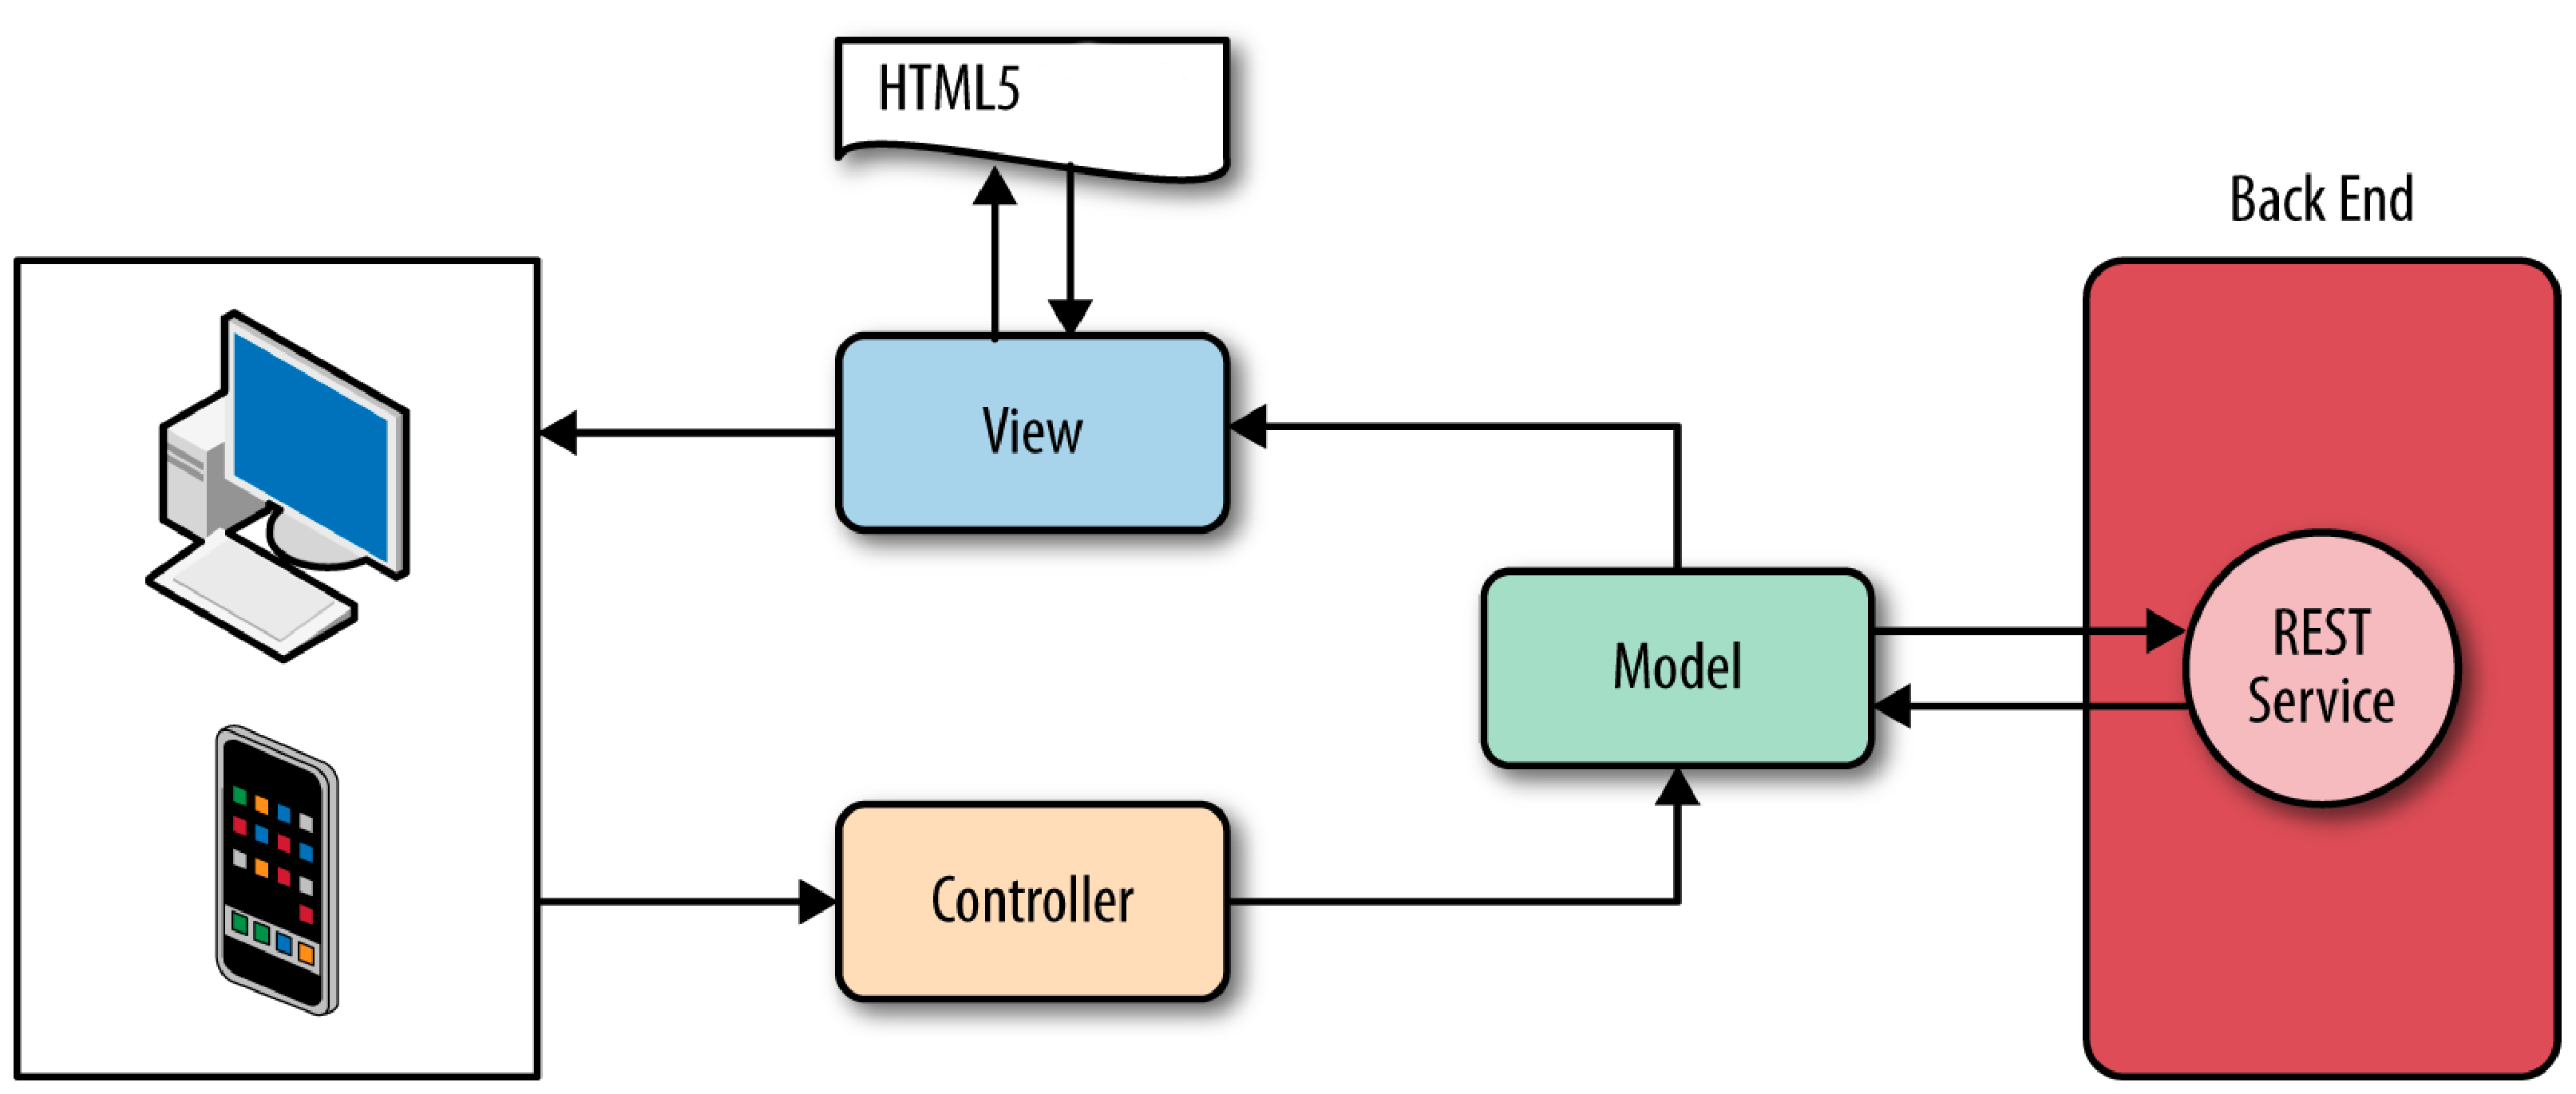
\includegraphics[width=14cm]{figuras/angulajs_mvc.eps}
	\caption{Diagrama de uma aplicação \emph{MVC} usando \emph{AngularJS}.}
	\label{angularjs_mvc}
	\footnotesize Fonte: \citeonline{Williamson2015}.
\end{figure}

Segundo \citeonline{Williamson2015}, a Figura \ref{angularjs_mvc} mostra o diagrama de uma aplicação \emph{AngularJS} e os componentes \emph{MVC}.  Uma vez que a aplicação é lançada, os componentes \emph{model, view} e \emph{controller}, juntamente com todos os documentos \emph{HTML} são carregados no \emph{desktop} ou \emph{smartphone} do usuário e rodam completamente num destes hardwares.  A aplicação \emph{AngularJS} conversa com o \emph{backend} via o protocolo \emph{http}.  O \emph{backend} é um servidor \emph{web} que mantém chamadas \emph{REST} (explicado na seção \ref{servicos_rest}), sendo responsável pela execução da lógica e de processos de negócio.  
Outra característica bastante apreciada pelos desenvolvedores que usam \emph{AngularJS}, é a possibilidade de criar \emph{single-page aplications (SPA)}. 
\emph{SPAs} são aplicações que tem uma página \emph{HTML} de entrada. 
Esta página tem seu conteúdo dinamicamente adicionado e removido da mesma.
Esta abordagem permite criar aplicações bastante interativas, lembrando mesmo, aplicações \emph{desktop} escritas em linguagens como \emph{Visual Basic} e \emph{Delphi}.

\subsection{ORGANIZAÇÃO DE PROJETOS WEB COM \emph{ANGULAR-SEED}}
\label{angular_seed}

O \emph{angular-seed}, é um \emph{template} para projetos \emph{web} que utilizam o \emph{AngularJS}. 
Ele facilita bastante o processo de configuração e padronização do projeto. 
Ele cria um \emph{layout} de diretórios padronizado, pré-configura as ferramentas de \emph{build} e também já pré-configura o ambiente de testes unitários \emph{web/javascript} usando a ferramenta \emph{JASMINE}. 
Mais informações sobre o \emph{angular-seed} em \citeonline{Google2015b}.

A Figura \ref{seed} mostra o \emph{layout} inicial de diretórios que a ferramenta gera após ser clonada do \emph{Github}.

\begin{figure}[ht]
	\centering
	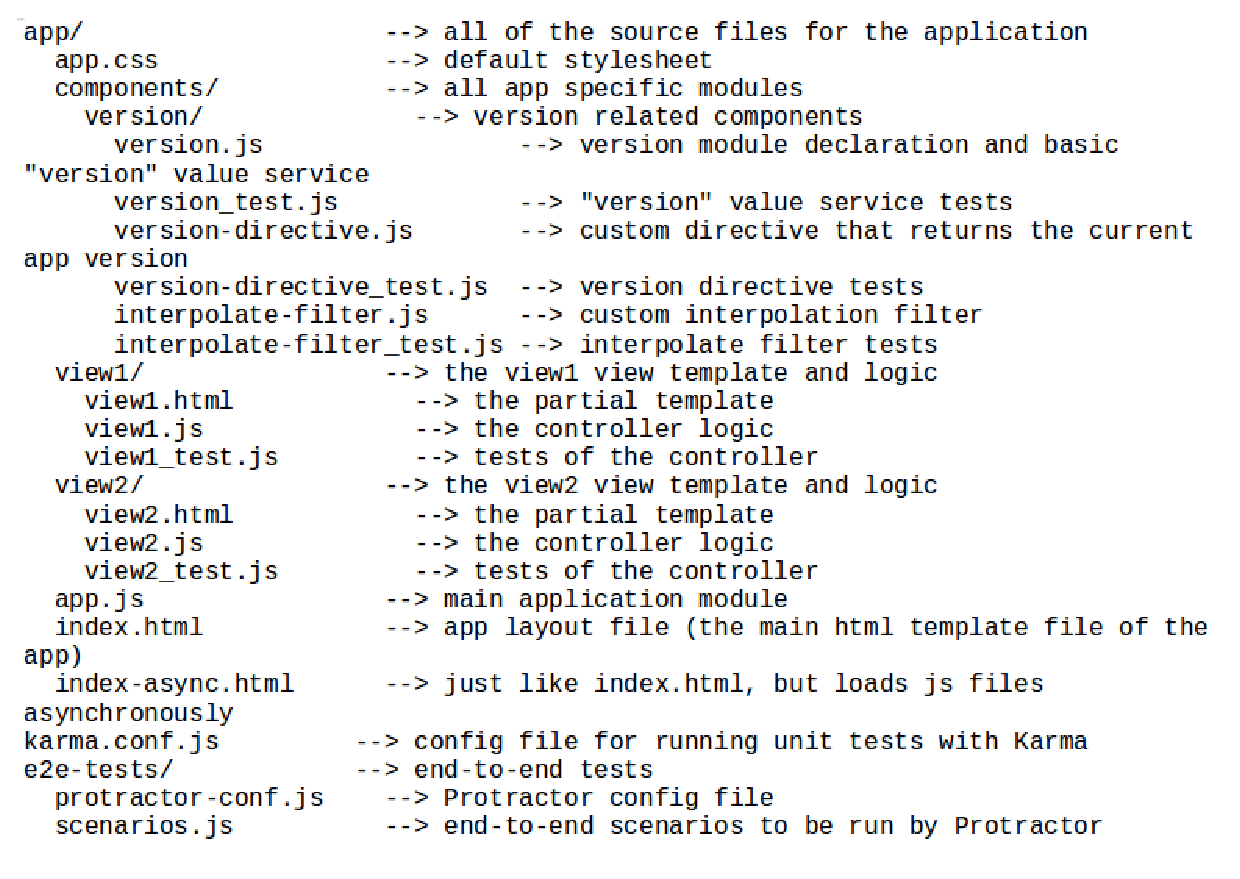
\includegraphics[width=14cm]{figuras/seed.eps}
	\caption{Layout original de um projeto baseado em \emph{angular-seed}. Fonte: \citeonline{Google2015b}.}
	\label{seed}
\end{figure}

Antes de começar a usar o \emph{angular-seed} é necessário instalar o ambiente de execução \emph{Javascript Node.JS}. 
Este ambiente é utilizado para execução de testes e construção de \emph{builds}. Para uma introdução ao \emph{Node.JS} veja \citeonline{Syed2014}.
\subsection{SOLUÇÃO DE DESIGN WEB COM \emph{ANGULAR-MATERIAL}}
\label{angular_material}

Os usuários profissionais da área de saúde, dificilmente se interessariam por um software complexo sem uma interface atraente e amigável.
Uma solução para minimizar este problema é a adoção da  biblioteca \emph{angular-material}. 
Esta biblioteca, como indicado pelo seu nome, é construída com o \emph{AngularJS}. 
Ela disponibiliza serviços e diretivas que podem ser usados para construir a interface gráfica da aplicação. 
Diretivas são componentes que podem ser inseridos diretamente no código HTML da aplicação, dando a aparência de estender a própria HTML. 
Por exemplo, a diretiva \emph{md-button} da biblioteca é um tipo de botão que não é próprio do HTML. 
Outros exemplos de diretivas são: caixas de diálogos, barras de ferramentas, barras de progresso, grades, \emph{tooltip}, etc. 
Esta biblioteca é baseada na especificação \emph{Material Design} criada pela empresa \emph{Google}. 
A especificação discorre sobre padrões de designe gráfico e interação com usuário e é baseada no princípio da metáfora de materiais. 
Esta metáfora é uma teoria unificada de um espaço racionalizado e sistemas de movimento, isto segundo \citeonline{Google2015a}. 
Outra vantagem da biblioteca é que ela é projetada para se adaptar a diferentes tipos de dispositivos com telas de tamanhos diferentes.
Veja um exemplo de aplicação que usa \emph{angular-material} na Figura~\ref{material_1}.


\begin{figure}[ht]
	\centering
	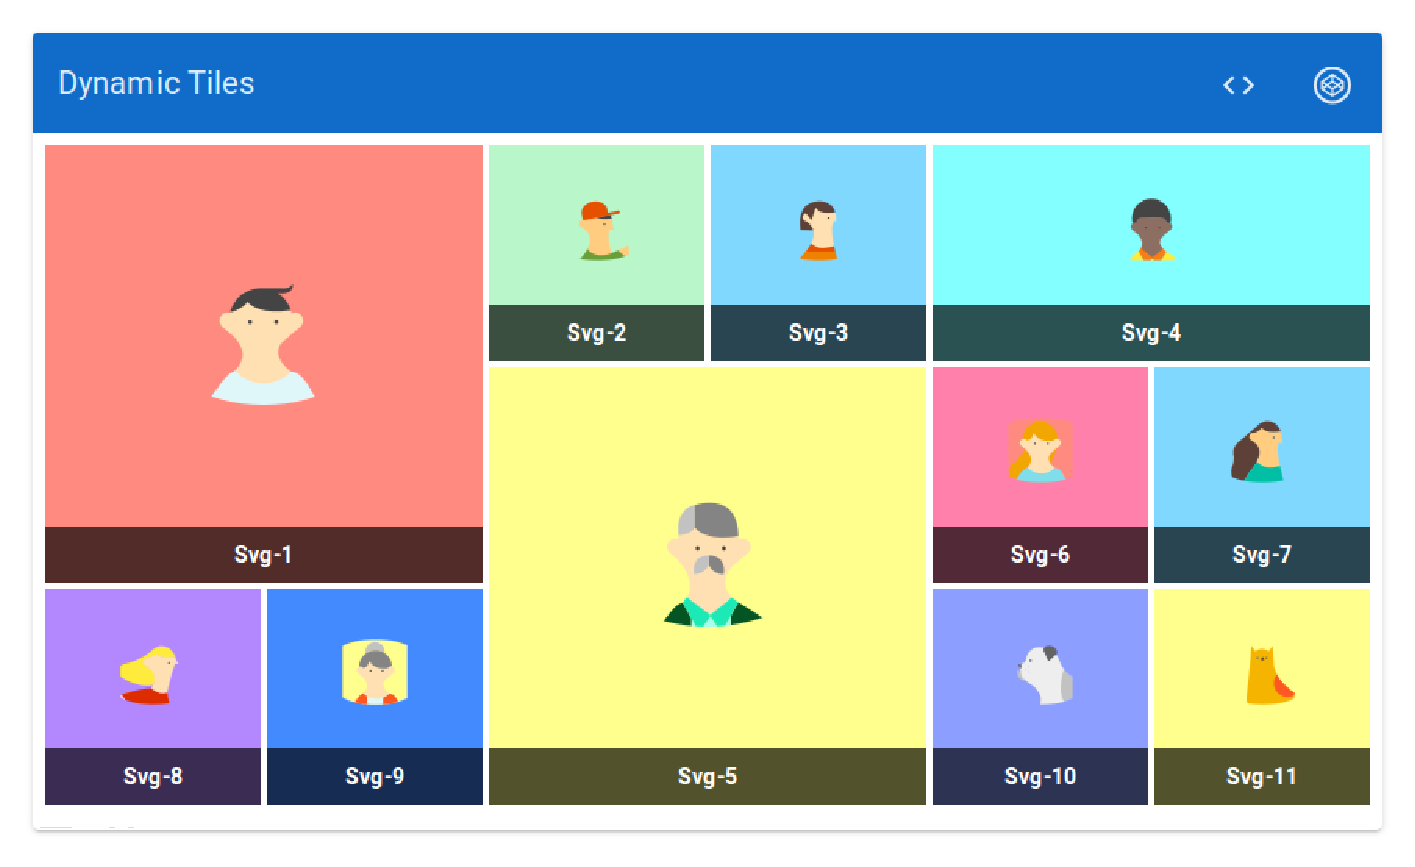
\includegraphics[width=14cm]{figuras/material.eps}
	\caption{Exemplo de aplicação que utiliza \emph{angular-material}. Fonte: \citeonline{Google2015c}.}
	\label{material_1}
\end{figure}



\subsection{GRÁFICOS E ANIMAÇÕES 3D NA \emph{WEB} COM \emph{THREEJS}} 
\label{threejs_sec}
Os \emph{browsers} modernos hoje, inclusive os dos \emph{smartphones}, suportam o novo padrão \emph{WebGL}. 
Este é um padrão \emph{web} multi-plataforma de \emph{API} de baixo nível para gráficos 3D, expostos através de \emph{HTML}. 
Este padrão suporta o acesso da \emph{API} usando-se a linguagem \emph{GLSL}. 
Uma vantagem desta API é que ela suporta nativamente \emph{GPUs} disponibilizadas pelo hardware que está executando o cliente \emph{web}. 
Isto torna possível até mesmo a criação de jogos de alta definição em 3D que rodam no \emph{browser} \cite{Matsuda2013}.

O problema com a \emph{WebGL} é que, como dito anteriormente, a \emph{API} é de baixo nível. 
No contexto de computação gráfica, isto significa que ela fornece primitivas básicas para modelagem 3D e outras opções de otimização do hardware.
Para resolver este problema bibliotecas em \emph{javascript} foram desenvolvidas, disponibilizando funções e objetos de alto nível, como cilindros, planos, esferas, animações, entre outros. 
Uma opção é o \emph{ThreeJS}, descrito em \citeonline{Dirksen2015}. 
Esta biblioteca apresenta um grande número de funcionalidades e é possível encontrar aplicações e jogos em 3D de nível profissional. 
Um exemplo de animação renderizada que utiliza \emph{ThreeJS} é mostrada na Figura \ref{evil_eye}.
Mais exemplos podem ser vistos no site \emph{threejs.org}.



\begin{figure}[H]
	\centering
	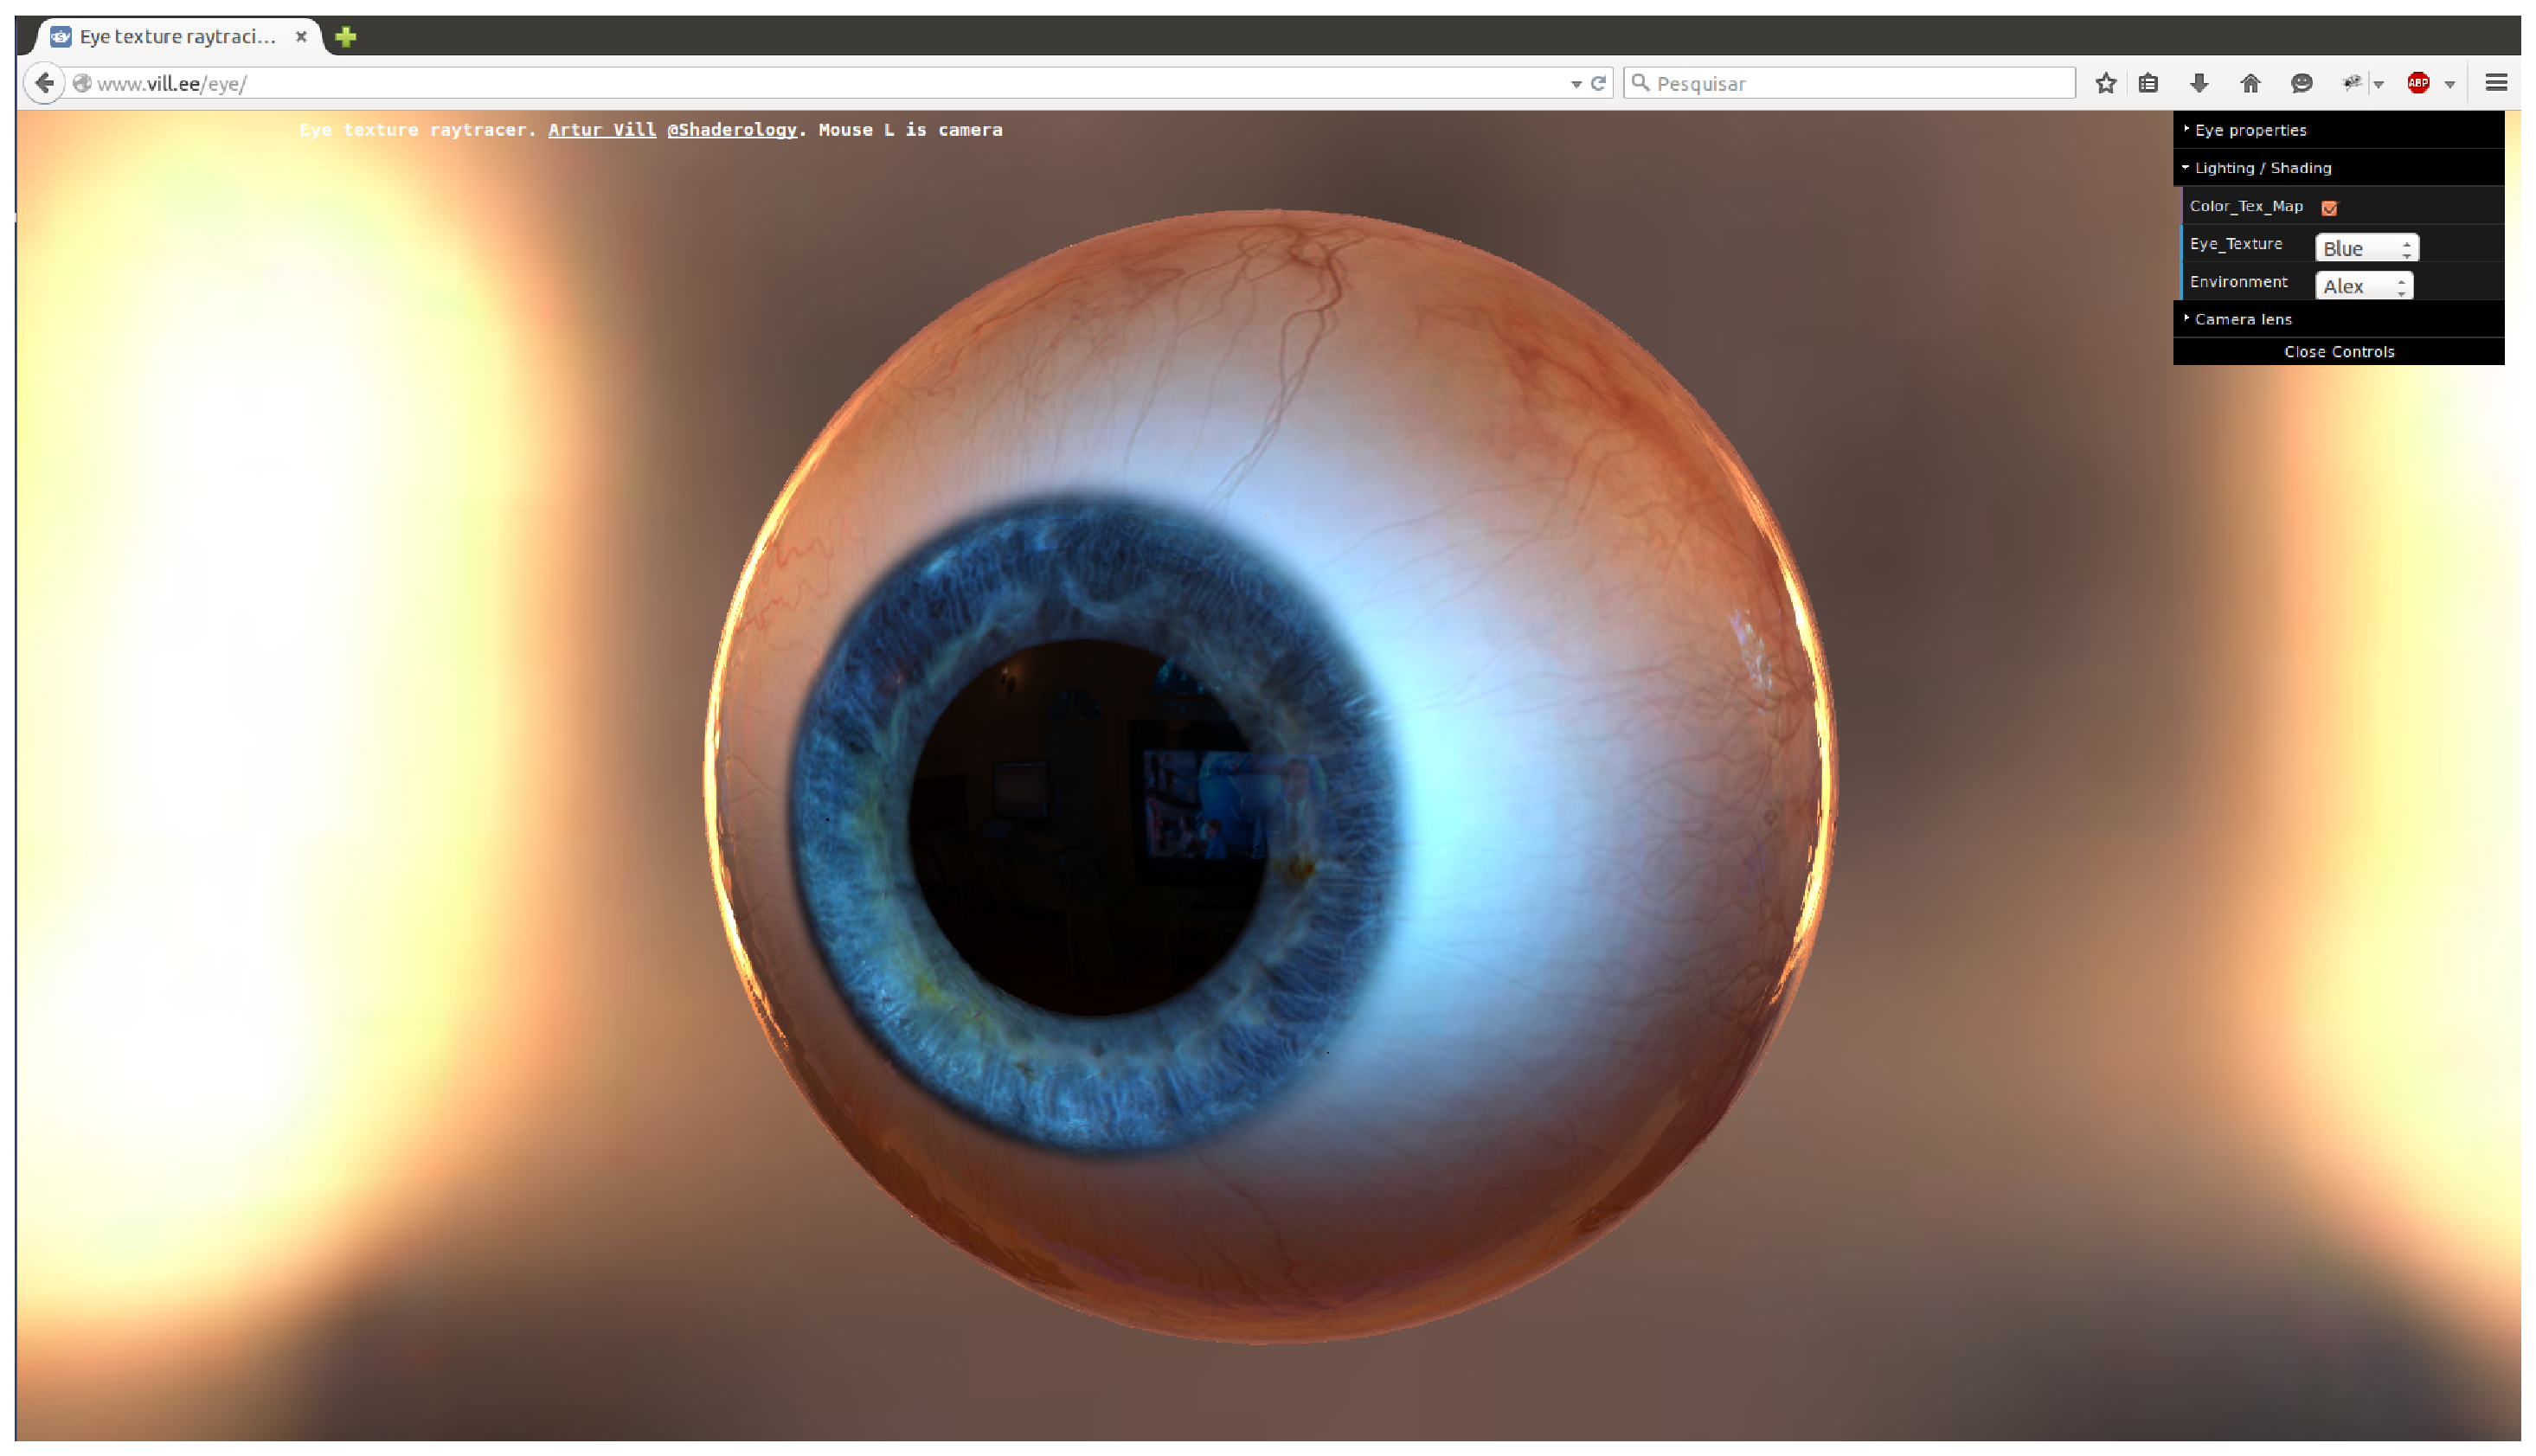
\includegraphics[width=14cm]{figuras/evil_eye.eps}
	\caption{Exemplo de aplicação que utiliza \emph{ThreeJS}.}
	\label{evil_eye}
	\footnotesize Fonte: \url{http://www.vill.ee/eye/}.
\end{figure}


\subsection{SERVIÇOS REST COM \emph{FLASK}}
\label{servicos_rest}

O \emph{Representational State Transfer (REST)} foi primeiramente descrito por \citeonline{Fielding2000}. 
Ele é definido como um estilo arquitetural de sistemas hipermídia e tem as seguintes características descritas por \citeonline{Grinberg2014}:

\begin{enumerate}
	\item Cliente-Servidor. Há uma separação clara entre quem consome, cliente, e quem serve e executa a lógica de negócio, servidor;
	\item \emph{Stateless}. O cliente precisa incluir nas suas requisições, todas as informações necessárias para o servidor processar o pedido. O servidor não armazena informações de estado do cliente entre as requisições deste;
	\item Interface Uniforme. O protocolo que os clientes usam para acessar o servidor precisa ser consistente, bem definido e padronizado. O protocolo comumente usado por serviços \emph{REST} é o \emph{HTTP};
	\item Sistema em Camadas. Servidores \emph{proxy}, \emph{caches} ou \emph{gateways}, podem ser inseridos entre clientes e servidores quando necessários, para melhorar a performance, confiabilidade e escalabilidade;
	\item Código Sob Demanda. Clientes podem opcionalmente fazer o \emph{download} de código do servidor e executá-lo em seu contexto.
\end{enumerate}

A principal ideia de serviços \emph{REST} é o fornecimento de recursos. 
Por exemplo, o cliente requere um usuário, blog, comentários, entre outros. 
Cada recurso deve possuir uma \emph{URL} que o identifica unicamente, por exemplo, http://www.minhaurl.com.br/usuario/123, onde 123 é um identificador único do usuário.

O funcionamento de uma \emph{Web API REST} é mostrado na Figura \ref{rest_api}. Nesta figura vê-se um cliente, que pode ser um \emph{browser web} ou outra aplicação \emph{mobile} ou uma aplicação web ou qualquer \emph{software} cliente que se comunique pelo protocolo \emph{HTTP}. Este cliente faz requisições para um software servidor, através de uma \emph{API} que foi exposta anteriormente. No lado servidor a chamada a API específica é processada e uma resposta é devolvida ao cliente.

\begin{figure}[ht]
	\centering
	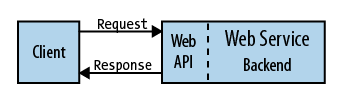
\includegraphics[width=7cm]{figuras/rest_api.eps}
	\caption{\emph{Web API REST}. Fonte: \citeonline{Masse2011}.}
	\label{rest_api}
\end{figure}


Para que um serviço \emph{REST} funcione, ele precisa ser implementado para suportar requisições \emph{HTTP}, ou seja, ele teria que ser um servidor \emph{web} completo. 
A biblioteca escolhida para desempenhar esta função foi a \emph{Flask}. 
Esta é uma biblioteca escrita na linguagem \emph{Python} e fornece todos as ferramentas necessárias para criar aplicações \emph{webs}. 
Segundo \citeonline{Maia2015}, o \emph{Flask} vem sendo adotado, por sua filosofia minimalista que não impõe uma arquitetura específica de projeto, assim permitindo que um projeto comece pequeno e simples, evoluindo para um modelo mais complexo.


\subsection{SERVIÇO DE BASE DE DOCUMENTOS COM \emph{MONGODB}}
\label{mongodb_sec}

Conforme \citeonline{Chodorow2013}, o \emph{MongoDB} é poderoso, flexível e um banco de dados de propósito geral bastante escalável. Ele combina a habilidade de alta escalabilidade com índices secundários, pesquisas limitadas, ordenamento, agregações e índices geoespaciais.

O \emph{MongoDB} é classificado como um banco \emph{NoSQL}. Segundo \citeonline{Dayley2014}, o conceito de \emph{NoSQL} consiste em tecnologias que provêm armazenamento e recuperação sem o amarrado modelo tradicional de bancos de dados Relacionais. A motivação para estas tecnologias é o design simplificado, escalabilidade horizontal e controle fino na disponibilidade dos dados.

O \emph{MongoDB} como toda grande ferramenta de software, foi designado baseado em filosofias próprias, que para os novatos, às vezes pode parecer um contrassenso. 
\citeonline{Plugge2014} comenta que o pináculo das filosofias do \emph{MongoDB} é a noção de que um tamanha não se adéqua a todos. Por muitos anos bancos de dados relacionais foram usados para armazenar conteúdos de todos os tipos. O principal motivo para isso é que ler e escrever em bancos de dados relacionais é muito mais seguro do que fazer o mesmo em arquivos de sistema operacional.
É comum no uso de bancos de dados relacionais, ter que se criar dezenas de tabelas para se armazenar dados complexos, e ainda tentar fazer todas funcionarem juntas.

Ainda, segundo \citeonline{Plugge2014}, a equipe do \emph{MongoDB} decidiu que não ia criar outro banco de dados para resolver todos os problemas do mundo. Eles criaram um banco que trabalha com documentos ao invés de linhas em tabelas. Essa decisão tornou o \emph{MongoDB} muito rápido, altamente escalável e fácil de usar. Por exemplo, o \emph{MongoDB} não suporta transações, logo você não irá escrever uma aplicação de conta corrente com ele. Sua força está armazenar dados muito complexos. No final o desenvolvedor ainda tem a opção de usar um banco de dados relacional que suporta transação e as vantagens do \emph{MongoDB} para outras partes da aplicação, que se aproveitarão melhor do modelo de documentos.


A Figura \ref{mongodb} mostra como os dados são organizados nesta tecnologia.

\begin{figure}[ht]
	\centering
	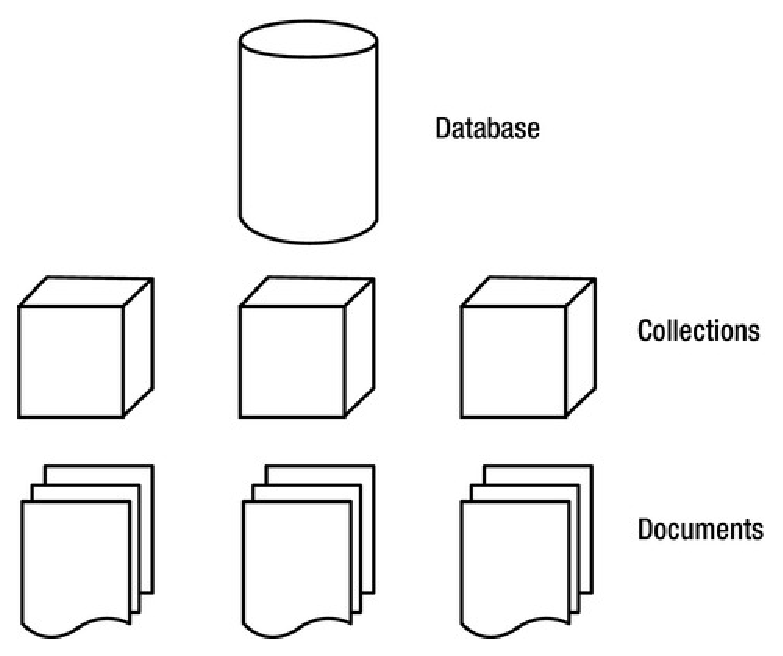
\includegraphics[width=10cm]{figuras/mongodb.eps}
	\caption{Organização dos dados no \emph{MongoDB}. Fonte: \citeonline{Plugge2014}.}
	\label{mongodb}
\end{figure}

Segundo a Figura \ref{mongodb}, um banco de dados \emph{MongoDB} é composto por coleções de dados. 
Dentro destas coleções existem documentos. 
Os documentos dentro de uma coleção não precisam ser do mesmo tipo. 
Mas esta é uma prática pouco recomendada \cite{Plugge2014}. 
Os documentos são armazenados no formato \emph{Binary Object Notation (BSON)}, um primo muito próximo do \emph{JavaScript Object Notation (JSON)}. 
O \emph{BSON} é muito parecido com o \emph{JSON}. Ele foi criado para ser mais otimizado nas leituras e escritas no banco. A Figura \ref{listagem1} retirada de \citeonline{Dayley2014}, mostra como um documento se parece.

\begin{figure}[H]
	\centering
	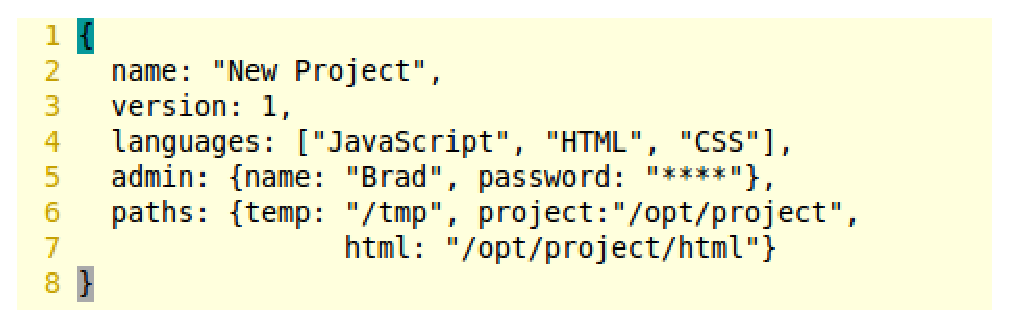
\includegraphics[width=12cm]{figuras/listagem1.eps}
	\caption{Listagem de um documento. Fonte: \citeonline{Dayley2014}.}
	\label{listagem1}
\end{figure}


Para quem conhece \emph{JSON}, provavelmente compreendeu todo o documento. Um documento fica entre \{\} e pode conter outros documentos, tipos simples e listas.
O documento possui atributos, no exemplo, \emph{name, version, languages, admin, paths}. Os atributos \emph{name version} são atributos de tipos simples, texto e número no caso. O atributo \emph{languages} é uma lista e os demais são outros objetos.

A questão da normalização dos objetos é sempre uma decisão do desenvolvedor. É perfeitamente possível tratar coleções e documentos, como tabelas. Como cada tabela tem um identificador único gerado pelo sistema é possível inclusive fazer referência entre documentos. Mas o ideal é encontra um meio termo, onde dados muito acessados juntamente, fiquem numa estrutura hierárquica como a da listagem acima \cite{Dayley2014}. A Figura \ref{normalizacao} mostra como se pode fazer a referência entre documentos.

\begin{figure}[ht]
	\centering
	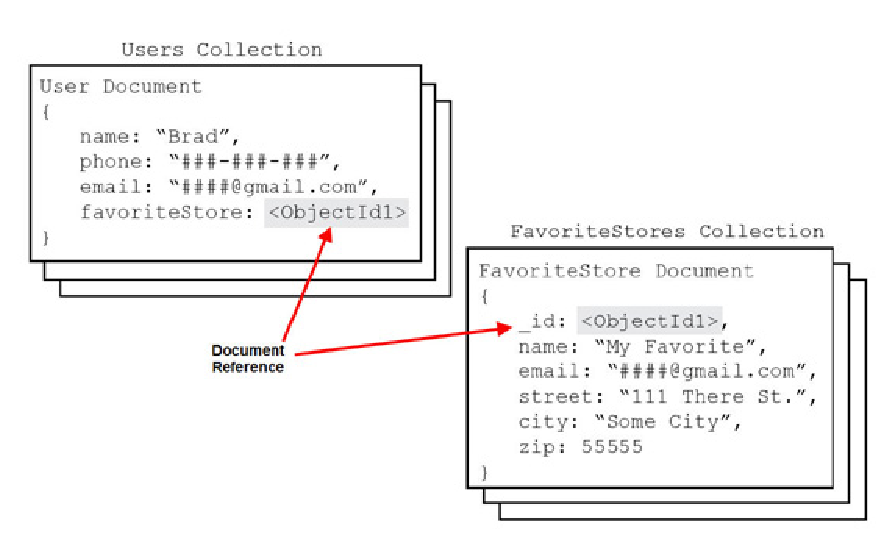
\includegraphics[width=12cm]{figuras/normalizacao.eps}
	\caption{Definindo documentos normalizado com \emph{MongoDB}. Fonte: \citeonline{Dayley2014}.}
	\label{normalizacao}
\end{figure}


\goodbreak
\newpage
\clearpage

\section[CMAC]{CMAC}
\label{cmac_sec}

A \emph{Cerebellar Model Articulation Controller} (CMAC) foi criada por James Sacra Albus \cite{Albus1975b}. 
Ele se inspirou no cerebelo dos mamíferos para criá-la. 
O mesmo autor havia feito um extenso trabalho sobre o funcionamento do cerebelo \cite{Albus1971b}.
Trabalho este, que resultou numa tese de doutorado \cite{Albus1972a}.
Aplicações da CMAC podem ser vistas em \cite{Albus1975d}, \cite{Albus1979}, \cite{Sabourin2006a} e \cite{Lin2002a}.
Uma aplicação que começou a ser desenvolvida pela UnB é descrita em \citeonline{Andrade2014}. Inclusive a implementação da \emph{CMAC} desenvolvida neste trabalho teve origem nele.

Na Figura \ref{fig1} é possível ver o funcionamento básico da CMAC. Os sinais $S$ entram no sistema, que mapeiam o mesmo para um conjunto de pesos $W^*$ que devem ser somados para ativação. 
Note que apenas uma pequena fração de pesos é realmente selecionada para participar na ativação. 
O conjunto de pesos disponíveis na CMAC é necessariamente maior que o número de pesos ativados $W^*$. 

\begin{figure}[H]
	\centering
	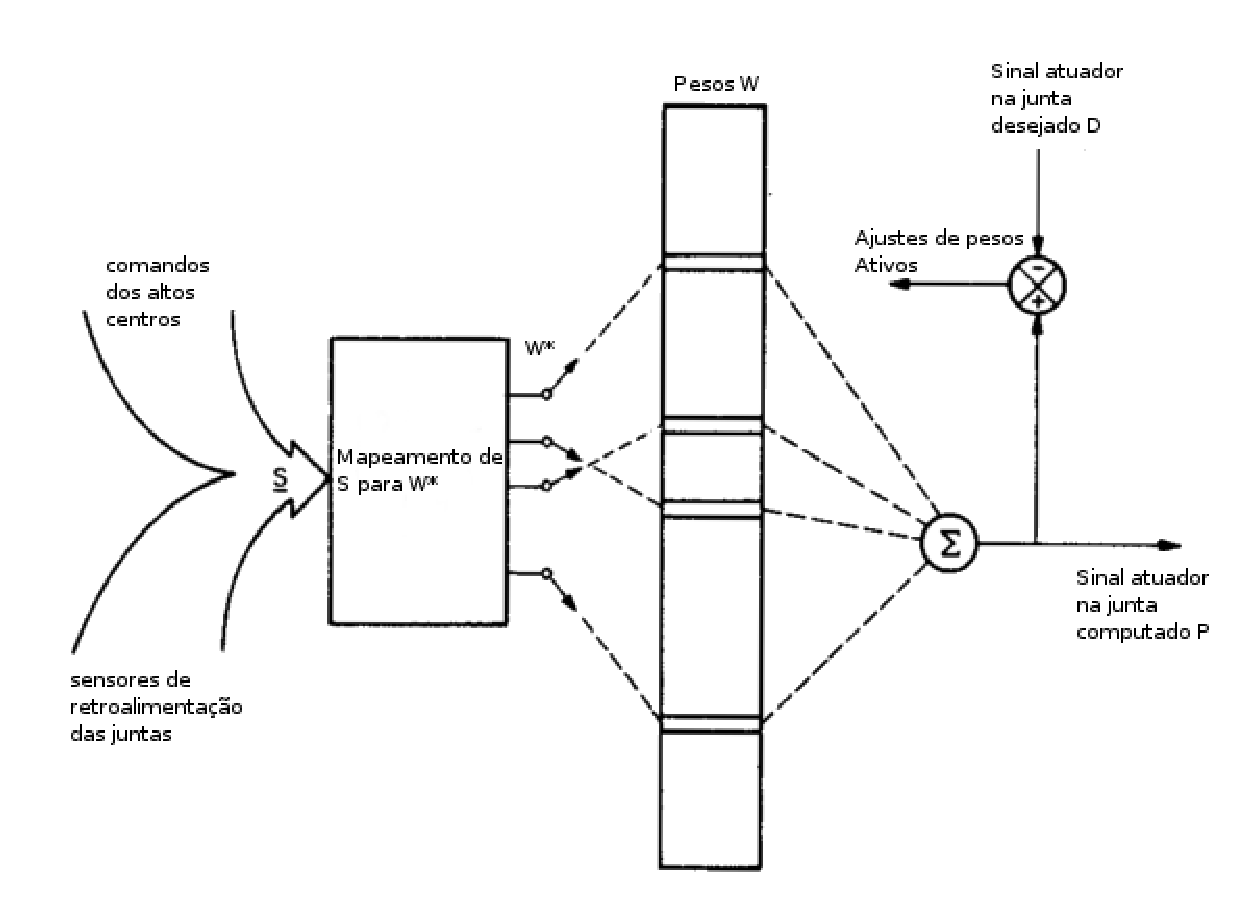
\includegraphics[width=15 cm]{figuras/cmac1.eps}
	\caption{CMAC para controle de uma junta. Fonte: Alterado de \citeonline{Albus1975b}.}
    	\label{fig1}
\end{figure}


A CMAC da Figura \ref{fig1} também pode ser classificada como um sistema \emph{Multiple Input Single Output} (MISO), ou seja, suporta a entrada de vários sinais de entrada e processa um sinal de saída.
Para se produzir uma CMAC \emph{Multiple Input Multiple Output} MIMO, bastaria implementar várias MISOs, compartilhando as mesmas entradas.


Os passos para que o sinal seja computado são descritos a seguir. Estes passos são os mesmos descritos em \citeonline{Albus1975b}.

Primeiramente, define-se o número de pesos $NW*$ a serem ativados para comporem a saída da CMAC.

O segundo passo é quantizar os possíveis valores para cada item do vetor de entrada $S$.
Por exemplo, se o primeiro item $s1$ de $S$ aceita valores de -1 até 1 e se quer 5 valores possíveis, quantiza-se então os valores de -1 até 1, conforme a Figura \ref{inputs1}.


\begin{figure}[ht]
	\centering
	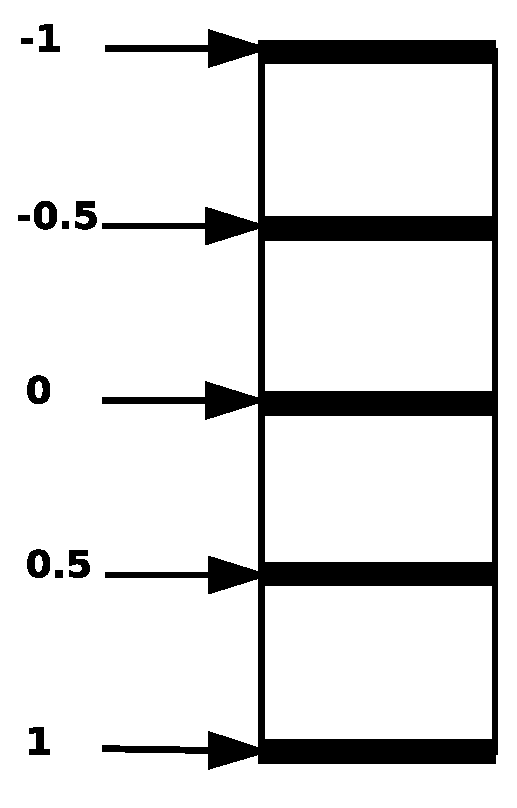
\includegraphics[width=3 cm]{figuras/input.eps}
	\caption{Quantização de $s1$.}
    	\label{inputs1}
\end{figure}


Isto significa que quaisquer que sejam os valores de $s1$ os mesmos devem ser convertidos para -1, -0,5, 0, 0,5 e 1. 
Por exemplo, se o valor de $s1$ for 0,75, será convertido para o valor 1, se for -0,75 será o valor 0 e se for 0,25 será o valor 0,5. A esta quantização dá-se o nome de resolução da CMAC \cite{Albus1975b}.

O próximo passo é criar uma tabela para cada um dos sinais discretizados de entrada do vetor $S$. 
Supondo que o vetor $S$ possui 2 sinais de entrada $s1$ e $s2$ e um número de ativações $NW*$ igual a 3, deve-se criar duas tabelas, uma para cada sinal, conforme se apresentam na Tabela \ref{disc_s1} e na Tabela \ref{disc_s2}. 
Para facilitar o entendimento, irá se considerar os valores possíveis de $s1$ iguais aos inteiros de 1 até 6 e os valores possíveis de $s2$ iguais aos inteiros de 1 até 4.
Cria-se uma coluna com os valores do sinal em questão. 
Para cada valor, cria-se 3 ($NW*$) valores novos. 
Para o primeiro valor do sinal, usa-se os 3 primeiros inteiros não negativos.
Para o segundo valor do sinal, substitui-se o primeiro dos três itens pelo próximo número após o terceiro item do sinal anterior. 
Para o terceiro sinal, substitui-se o segundo dos três itens pelo próximo inteiro não negativo.
Assim, sucessivamente conforme a Tabela \ref{disc_s1} e Tabela \ref{disc_s2} \cite{Albus1975b}.

\begin{table}[H]
	\centering
	\caption{Mapeamento de $s1$}
	\label{disc_s1}
	\ABNTEXfontereduzida
	\begin{tabular}{c c}
		\toprule
		\textit{Valore de $s1$} & \textit{Mapeamento $m1$}\\
		\midrule
		\ABNTEXfontereduzida
		1 & 0, 1, 2 \\
		2 & 3, 1, 2 \\
		3 & 3, 4, 2 \\
		4 & 3, 4, 5 \\
		5 & 6, 4, 5 \\
		6 & 6, 7, 5 \\
		\bottomrule
	\end{tabular}
\end{table}
\begin{table}[H]
	\centering
	\caption{Mapeamento de $s2$}
	\label{disc_s2}
	\ABNTEXfontereduzida
	\begin{tabular}{c c}
		\toprule
		\textit{Valore de $s2$} & \textit{Mapeamento $m2$}\\
		\midrule
		\ABNTEXfontereduzida
		1 & 0, 1, 2 \\
		2 & 3, 1, 2 \\
		3 & 3, 4, 2 \\
		4 & 3, 4, 5 \\
		\bottomrule
	\end{tabular}
\end{table}


Depois de mapeado cada valor de cada item de entrada, deve-se combinar os mapeamentos de acordo com a Tabela \ref{wmap}.

\begin{table}[ht]
	\centering
	\caption{Mapeamento para os pesos $W$}
	\label{wmap}
	\ABNTEXfontereduzida
	\begin{tabular}{c c c c c}
		\toprule
		\textit{$s1$ / $s2$} & \textit{1}  & \textit{2} & \textit{3} & \textit{4} \\
		\midrule
		\ABNTEXfontereduzida

		\textit{1} & (0, 0), (1, 1), (2, 2) & (0, 3), (1, 1), (2, 2) & (0, 3), (1, 4), (2, 2) & (0, 3), (1, 4), (2, 5) \\
		\textit{2} & (3, 0), (1, 1), (2, 2) & (3, 3), (1, 1), (2, 2) & (3, 3), (1, 4), (2, 2) & (3, 3), (1, 4), (2, 5) \\
		\textit{3} & (3, 0), (4, 1), (2, 2) & (3, 3), (4, 1), (2, 2) & (3, 3), (4, 4), (2, 2) & (3, 3), (4, 4), (2, 5) \\
		\textit{4} & (3, 0), (4, 1), (5, 2) & (3, 3), (4, 1), (5, 2) & (3, 3), (4, 4), (5, 2) & (3, 3), (4, 4), (5, 5) \\
		\textit{5} & (6, 0), (4, 1), (5, 2) & (6, 3), (4, 1), (5, 2) & (6, 3), (4, 4), (5, 2) & (6, 3), (4, 4), (5, 5) \\
		\textit{6} & (6, 0), (7, 1), (5, 2) & (6, 3), (7, 1), (5, 2) & (6, 3), (7, 4), (5, 2) & (6, 3), (7, 4), (5, 5) \\

		\bottomrule
	\end{tabular}
\end{table}
 


O mapeamento da Tabela \ref{wmap} é feito da seguinte forma \cite{Albus1975b}: 
Coloca-se cada valor quantizado de $s1$ nomeando cada uma das linhas da tabela. 
Coloca-se cada valor discretizado de $s2$ nomeando cada uma das colunas das tabelas. 
Cada célula da tabela é obtida recuperando-se os itens de $s1$ e de $s2$, que estão na Tabela \ref{disc_s1} e na Tabela \ref{disc_s2}, e concatenando-se cada item de acordo com sua posição. 
Por exemplo, para o valor de $s1$ igual a 5, recuperam-se os itens (6, 4, 5), para o valor de $s2$ igual a 2, recuperam-se os itens (3, 1, 2). 
Agora é só criar novos itens, na mesma quantidade do valor $NW*$, concatenando-se cada item de acordo com sua posição. O lista resultante é ((6, 3), (4, 1), (5, 2)). 

Cada vetor de 2 posições da Tabela \ref{wmap}, por exemplo (0, 0), (4, 1), é um rótulo de uma entrada na tabela de pesos $W$.

Para se calcular a saída do sistema, suponha que os valores de $s1$ e $s2$, ainda sejam 5 e 2, respectivamente, e $NW*$ ainda seja 3. 
Neste caso, recupera-se o item da linha 5 e da coluna 2, que é ((6, 3), (4, 1), (5, 2)). 
Agora é acessada a tabela de pesos W e são recuperados os pesos cujas chaves são (6, 3), (4, 1) e (5, 2). 
Note-se que serão recuperados exatamente 3 pesos, que é exatamente o número de ativações $NW*$ desejadas. 
Os valores recuperados constituem um vetor chamado $W*$. A saída é calculada somando-se os valores de W*.



\subsection{TREINAMENTO DA CMAC}
Sendo a CMAC uma Rede Neural Artificial (RNA) com aprendizado supervisionado, seus pesos podem ser atualizados simplesmente computando-se o erro e atualizando-se apenas os pesos que participaram do computo do sinal $P$ \cite{Haykin1998}. O processo é detalhado nos próximos parágrafos.

Para se treinar a CMAC, primeiro define-se o conjunto de dados para treinamento que devem ser usados. 
Pode ser usado algo entre 20\% e 50\% dos dados coletados para desenvolvimento do sistema. 
Cada item destes dados deve conter um vetor de sinais de entradas $S$ e a resposta desejada $D$ para estes sinais. 
A tabela de pesos deve ser inicializada com valores randômicos. 
Para cada vetor $S$ deve ser calculado o vetor $W*$, que contém os endereços dos pesos a serem ativados. 
Calcula-se, então, a saída da rede $P$ para o vetor $S$, conforme definido no item \ref{cmac_sec}, somando os itens do vetor $W$. 
Atualizam-se os pesos sinápticos conforme a Equação \ref{write_weight} adaptada de \citeonline{Sabourin2012a}.
\begin{equation}
	\label{write_weight}
	w_{i} = w_{i} + \cfrac{\alpha (D - P)}{NW^{*}}
\end{equation}

A variável $w_{i}$ é um item qualquer dentro da tabela de pesos $W$. 
Em cada iteração no conjunto de dados para treinamento, deve-se atualizar apenas os pesos descritos em $W*$ naquele momento. 
A variável $\alpha$ é o coeficiente de aprendizado, deve ser um valor entre 0 e 1. 
A variável $NW*$ é o número de valores a serem utilizados para ativação, que consequentemente equivale ao número de itens do vetor $W*$.

Deve-se determinar o número de iterações \emph{batch} para o sistema. 
Uma iteração \emph{batch} consiste no processamento dos pesos para cada item dentro do conjunto de dados para treinamento \cite{Ng2015}. 
O sistema deve continuar iterando até atingir o número de iterações \emph{batch}.

Apesar do número de iterações \emph{batch} ser válido como critério de parada para o treinamento da CMAC, nada impede o uso de outros critérios, por exemplo, o erro quadrado médio da saída $Y$ em relação ao desejado $D$.

\section{ALGUNS CÁLCULOS CINEMÁTICOS}
\label{cinematica}
Para este trabalho ser concluído, alguns cálculos cinemáticos foram necessários. Os cálculos são  as velocidades, ângulos e velocidades angulares.

Velocidades entre duas posições adjacentes num espaço 3D, são calculadas conforme a Equação \ref{v_i} \cite{Poole2011}.
\begin{equation}
	\label{v_i}
	\overrightarrow{\nu} =  \cfrac{\overrightarrow{s2} - \overrightarrow{s1}}{\tau}
\end{equation}

Os vetores $\overrightarrow{s1}$ e $\overrightarrow{s2}$ são dados espaciais em três dimensões $(X, Y, Z)$ e $\tau$ é o tempo transcorrido entre o deslocamento de um ponto ao outro. O vetor $\overrightarrow{\nu}$ possui as velocidades calculadas.

Para o cálculo de ângulos em três dimensões, primeiro os componentes devem ser transladados para uma origem comum, assim é possível usar a 
Equação \ref{angulo} como descrita em \citeonline{Edwards2006}. 
Para tal, usam-se as Equações \ref{eq1} e \ref{eq2} \cite{Poole2011}.

\begin{equation}
	\label{eq1}
	\overrightarrow{c1}^\prime =  \overrightarrow{c1} - \overrightarrow{o}
\end{equation}
\begin{equation}
	\label{eq2}
	\overrightarrow{c2}^\prime =  \overrightarrow{c2} - \overrightarrow{o}
\end{equation}

As variáveis $\overrightarrow{c1}$, $\overrightarrow{c2}$ e $\overrightarrow{o}$, são vetores representando pontos no espaço. 
O vetor $\overrightarrow{o}$ é a origem dos dois seguimentos de reta que chegam a $\overrightarrow{c1}$ e $\overrightarrow{c2}$ cada um. 
No contesto deste trabalho, $\overrightarrow{c1}$ poderia ser um ponto na coxa, $\overrightarrow{c2}$ um ponto na tíbia e $\overrightarrow{o}$ um ponto no joelho. 
Assim seria possível calcular o ângulo de um joelho, por exemplo. Veja a Figura~\ref{leg}. 
As variáveis $\overrightarrow{c1}^\prime$ e $\overrightarrow{c2}^\prime$, são os vetores transladados e prontos para se calcular o ângulo de acordo com a Equação \ref{angulo} \cite{Edwards2006}.

\begin{figure}[H]
	\centering
	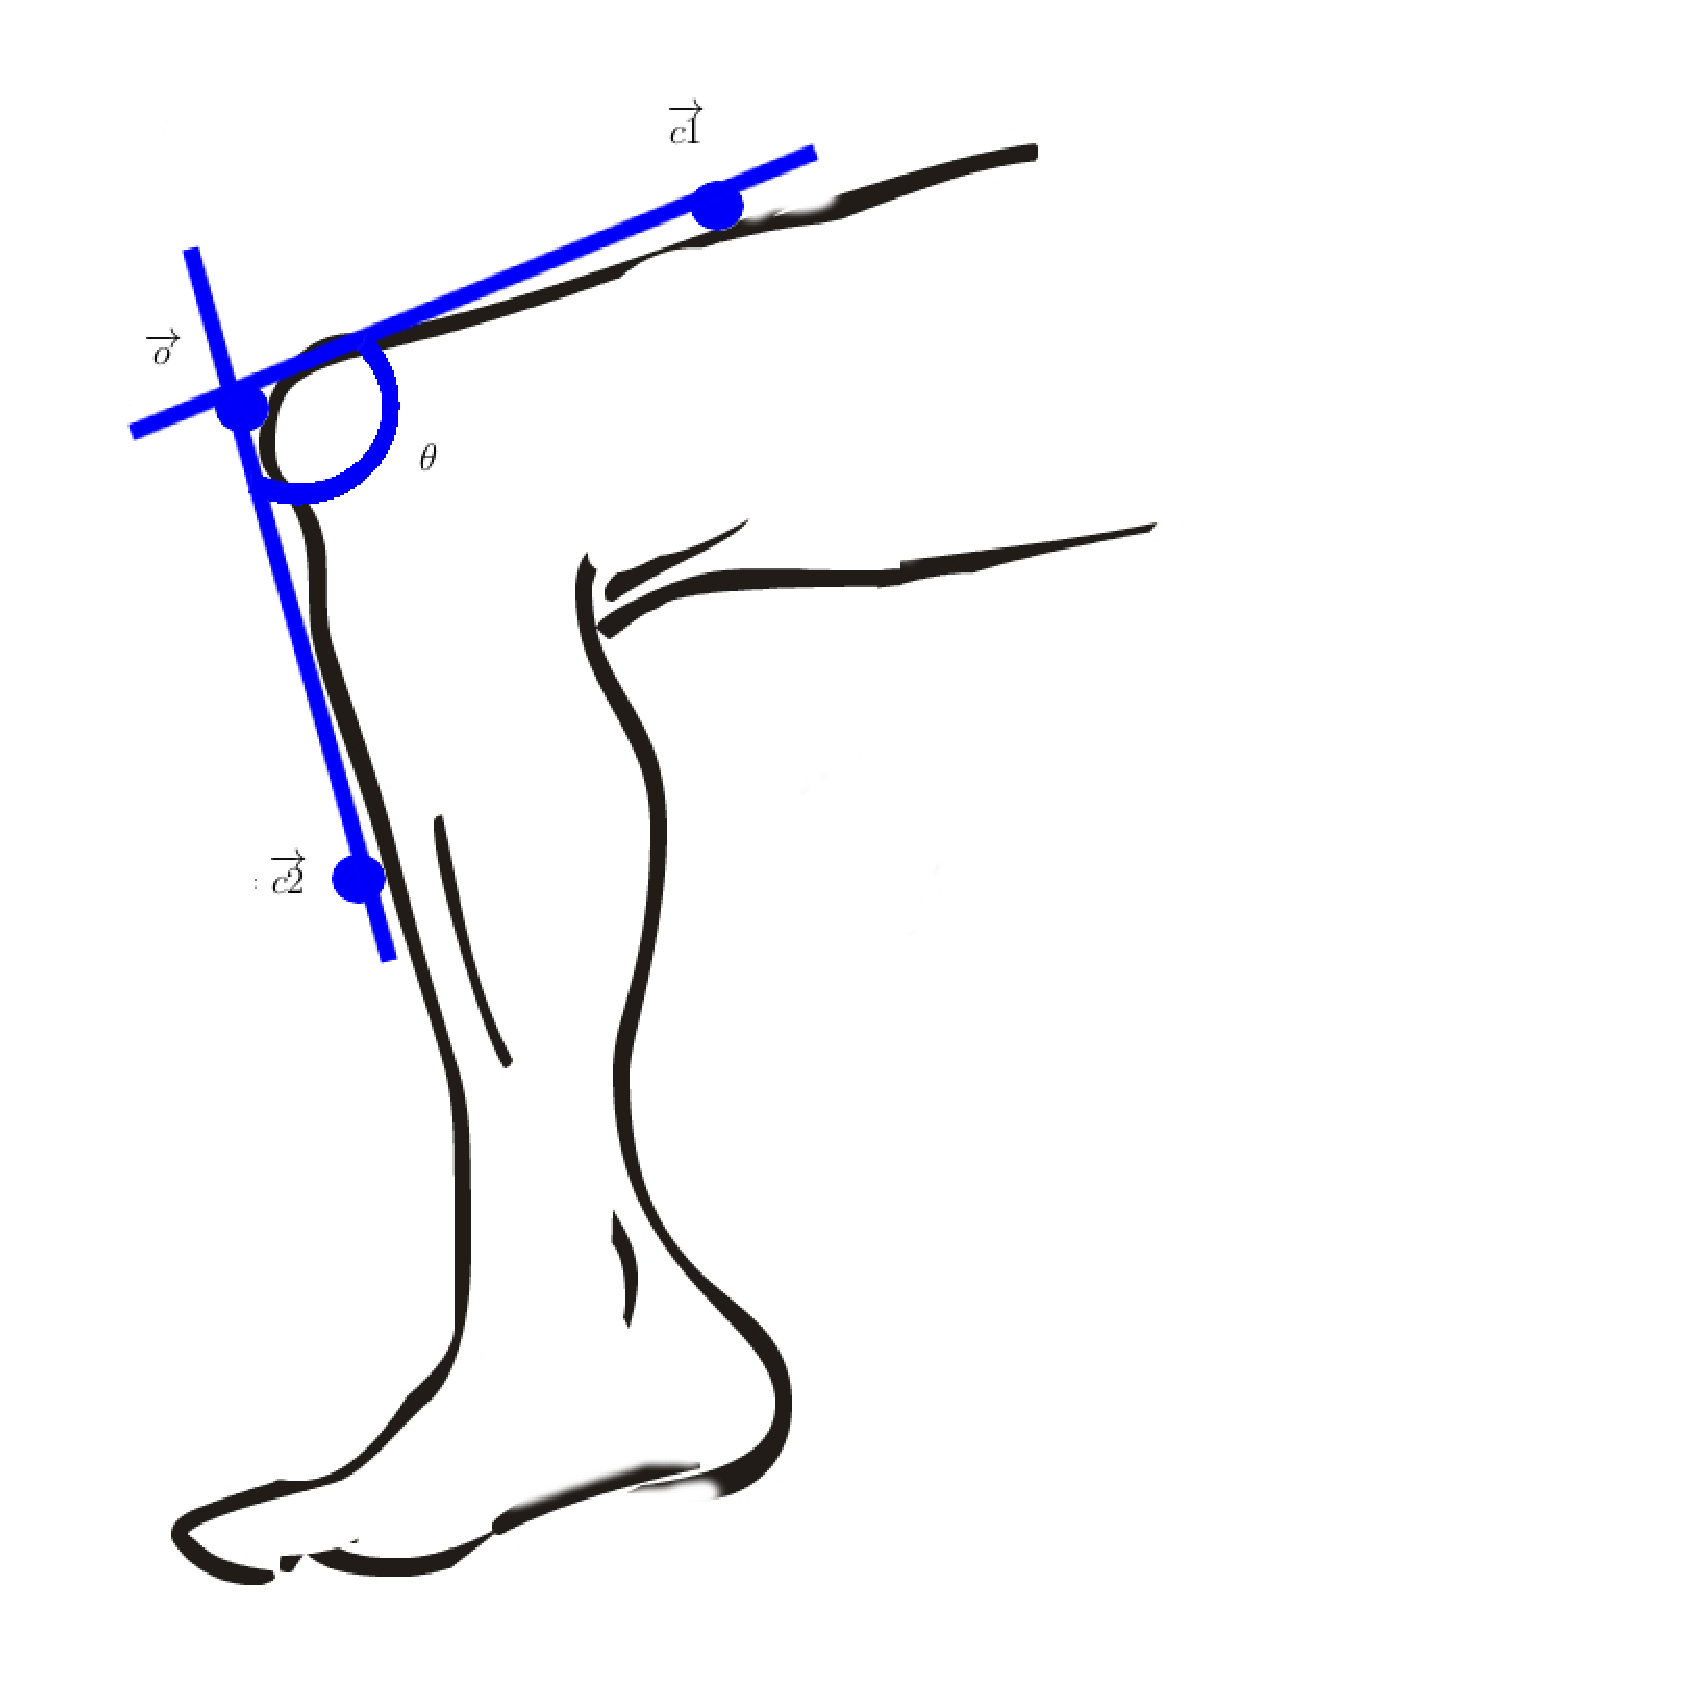
\includegraphics[width=14cm]{figuras/leg.eps}
	\caption{Exemplo hipotético de um ângulo. Fonte: Alterado de \citeonline{Cliparts2015}.}
	\label{leg}
\end{figure}


\begin{equation}
	\label{angulo}
	\theta = \arccos{(\frac{\overrightarrow{c1}^\prime.\overrightarrow{c2}^\prime} 
	{  \left \| \overrightarrow{c1}^\prime \right \|. \left \| \overrightarrow{c2}^\prime \right \|} )} 
\end{equation}

A variável $\theta$ é um ângulo em radianos.
O operador  $\left \| \right \|$ é a distância euclidiana como definida por \citeonline{Poole2011} e seu calculo é mostrado na Equação \ref{dist_e}.

\begin{equation}
	\label{dist_e}
	  \left \| \overrightarrow{c} \right \|  =  \sqrt{\overrightarrow{c} . \overrightarrow{c}}
\end{equation}

A velocidade angular é calculada segundo a Equação \ref{vel_ang} \citeonline{Poole2011}.


\begin{equation}
	\label{vel_ang}
	\omega =  \frac{\theta_2 - \theta_1}{\tau}
\end{equation}

A variável $\omega$ é a velocidade angular em radianos por segundo, $\theta1$ e $\theta2$ são ângulos e $\tau$ o tempo transcorrido entre a medida do primeiro ângulo e do segundo.



\section{SIMULAÇÃO} 

Segundo \citeonline{Garcia2009b} simulação é:

\begin{citacao}
A obtenção da resposta temporal das variáveis de interesse (variáveis dependentes) de um modelo, quando se excita suas variáveis de entrada com sinais desejados e se definem os valores das condições iniciais das variáveis dependentes.
\end{citacao}

A Figura \ref{simulacao} representa um modelo simplificado de um processo passível de simulação, onde $X$ é conjunto de variáveis de entrada, $Y$ é o conjunto de variáveis de saída e $P$ são os parâmetros do sistema incluindo condições de contorno. 
Com base neste modelo, \citeonline{Garcia2009b} afirma que é possível simular as seguintes aplicações:
\begin{enumerate}
	\item Projeto de equipamentos, processos e plantas e seus respectivos sistemas de controle;
	\item Pré-operação e operação de plantas;
	\item Sistema de controle de processos;
	\item Otimização das condições operacionais de plantas.
\end{enumerate}


\begin{figure}[ht]
	\centering
	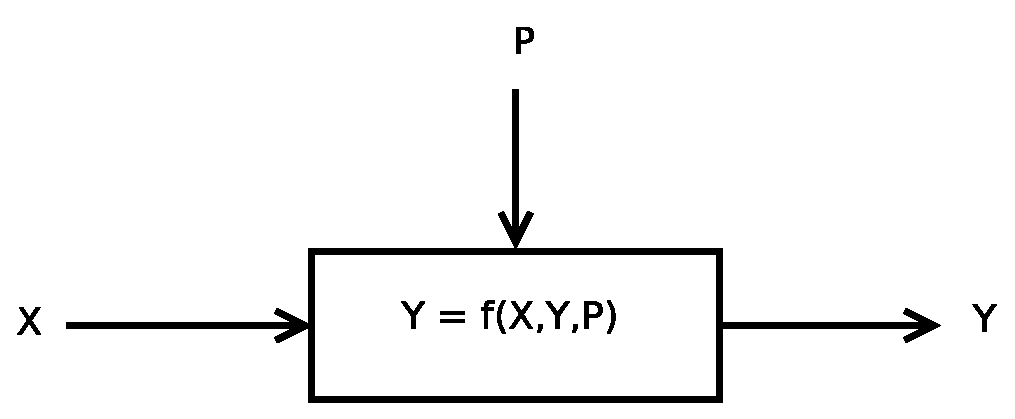
\includegraphics[width=10 cm]{figuras/simulacao.eps}
	\caption{Modelo matemático simplificado de um processo. Fonte: \citeonline{Garcia2009b}.}
    	\label{simulacao}
\end{figure}



\chapter[METODOLOGIA]{\textbf {metodologia}}

\section[AMBIENTE DE ESTUDO]{AMBIENTE DE ESTUDO}

Como este trabalho trata de um projeto de desenvolvimento de software na área de análise de marcha, dois ambientes de trabalho distintos foram amplamente utilizados. São estes:

\begin{enumerate}
	\item Laboratório de Informática em Saúde (LIS) na Faculdade Gama (FGA) da Universidade de Brasília (UnB);
	\item Laboratório de Performance Humana (LPH) na Faculdade Ceilândia (FCE) da UnB.
\end{enumerate}

No LIS foram desempenhadas as tarefas relativas a engenharia de software e disponibilização do software.
Foram utilizadas estações de trabalho do tipo \emph{Power Mac} com sistema operacional \emph{MAC OS X} 10.10.3, sendo que uma foi preparada para funcionar como servidor de aplicação e roteador de rede. 
A estação preparada serve de hospedeira de duas máquinas virtuais (\emph{Virtual Machines} - VMs) rodando através do software \emph{Virtualbox} 4.3. 
Cada VM utiliza sistema operacional \emph{Debian Wheezy GNU/Linux}. 
Uma destas VMs foi configurada como roteador e \emph{firewall} e a outra como servidor de aplicações.  
Outra estação de trabalho \emph{Power Mac}, idêntica, e um \emph{notebook} rodando \emph{Ubuntu 14.04 GNU/Linux} foram utilizados como máquinas de desenvolvimento e simulação.
Um diagrama da rede criada no LIS é mostrado na Figura \ref{lis_rede}.

\begin{figure}[ht]
	\centering
	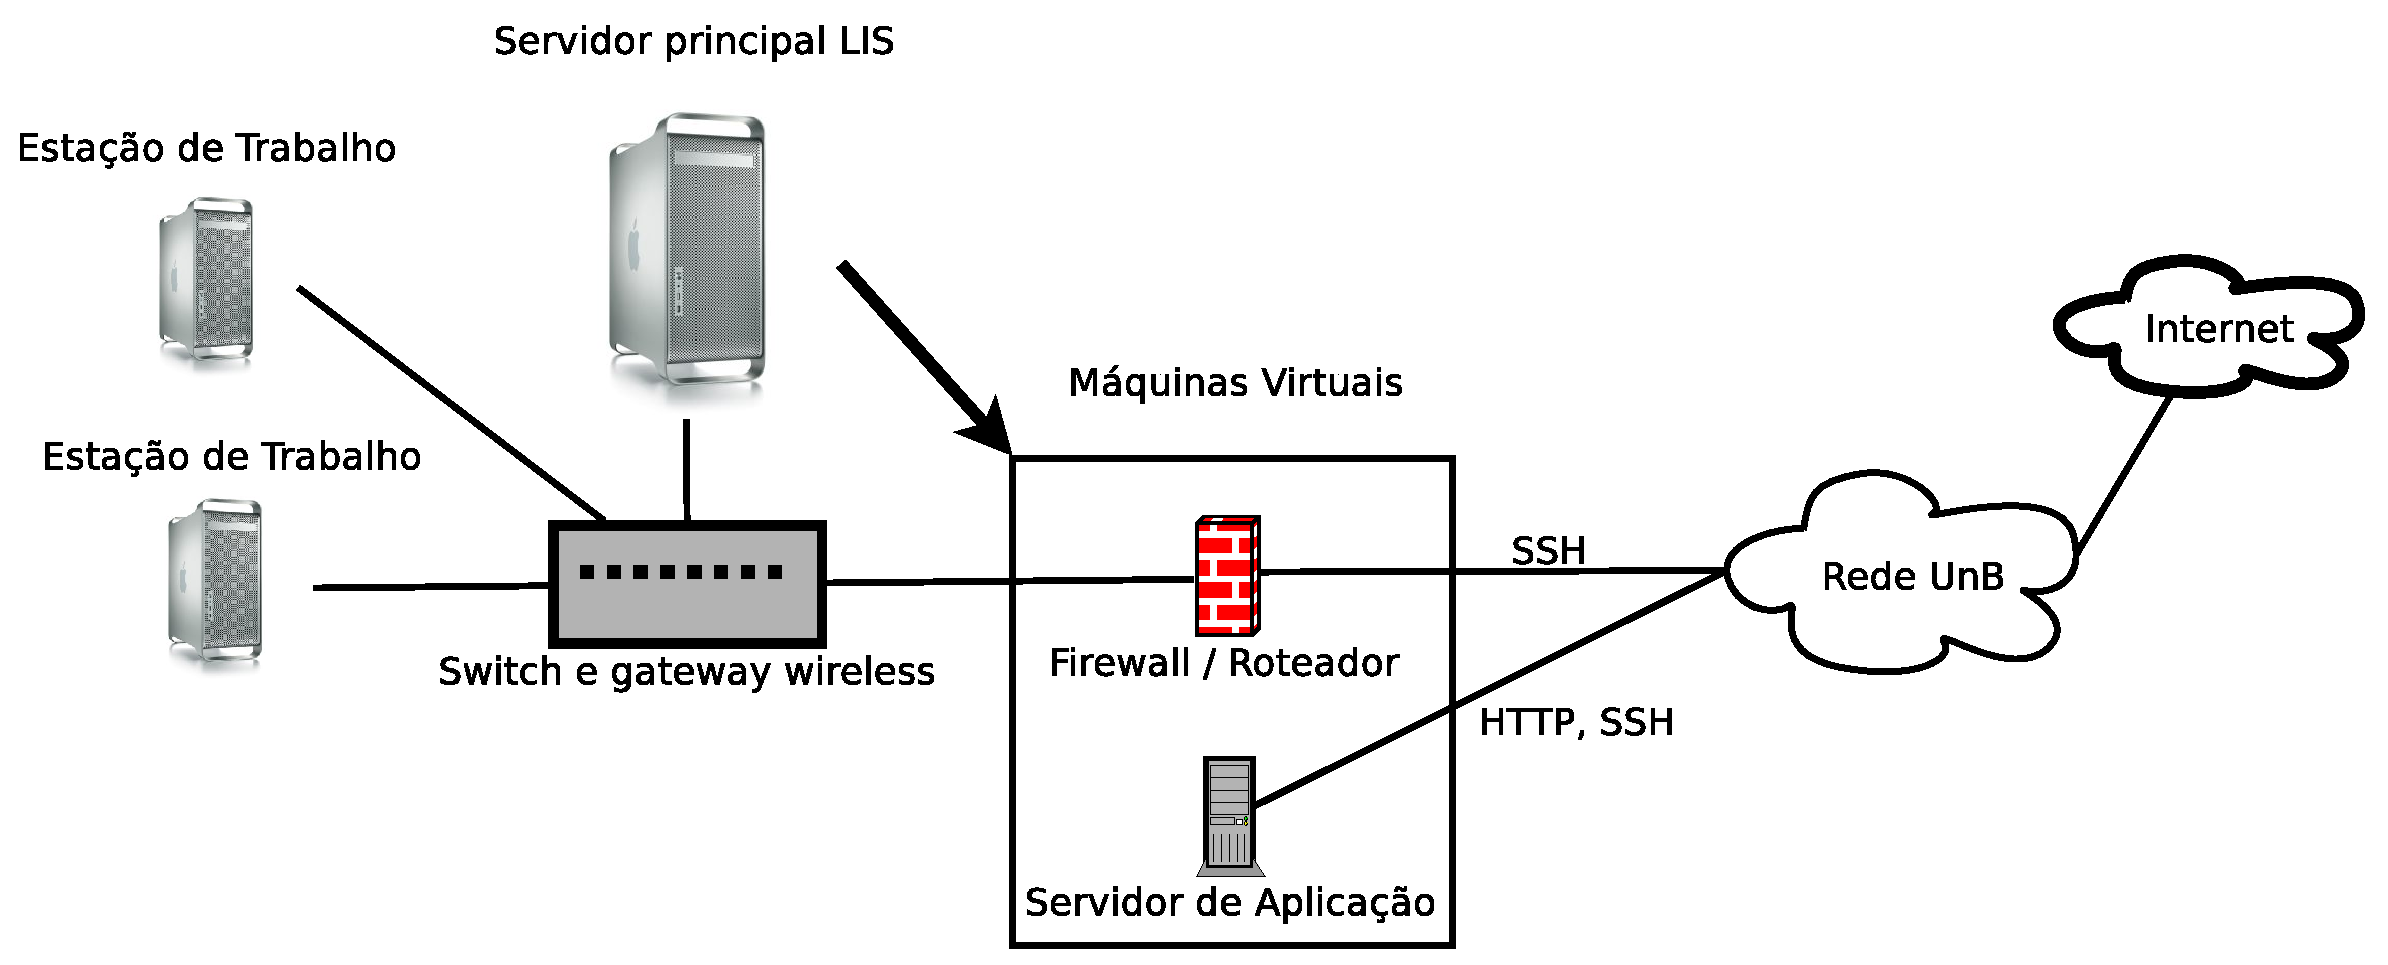
\includegraphics[width=15cm]{figuras/lis_rede.eps}
	\caption{Rede LIS.}
	\label{lis_rede}
\end{figure}

O LPH/FCE foi utilizado para captura de dados de marcha humana. 
Este laboratório está equipado para coletar dados de plataformas de força, eletromiógrafos e de marcadores passivos posicionados no corpo do paciente através de câmeras de vídeo \emph{Oqus-MRI}, usando técnicas de (\emph{Motion Capture - MOCAP}), ver Figura \ref{oqus_mri} na Seção \ref{metodos_analise}. 
Para este trabalho foi utilizado o software \emph{QTM 3.2} da \emph{Qualisys}, ver Figura \ref{visao_qtm} na Seção \ref{metodos_analise}, que é responsável pela coleta de dados \emph{MOCAP}. 

O processo de coleta é demonstrado na Figura \ref{coleta}.

\begin{figure}[ht]
	\centering
	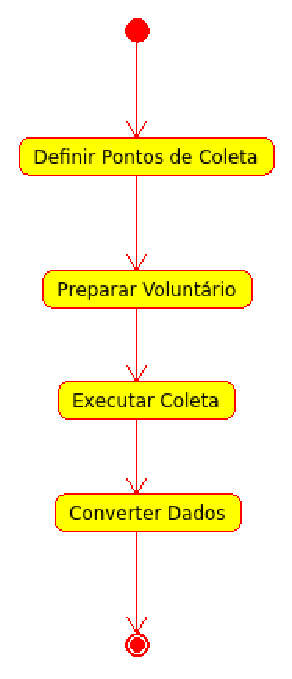
\includegraphics[width=5cm]{figuras/coleta.eps}
	\caption{Processo de coleta de dados.}
	\label{coleta}
\end{figure}

Primeiro deve-se definir o paciente da coleta e determinar o dia para este processo. 
Além disso, também é necessário definir quais os pontos no corpo do paciente devem receber marcadores de superfície. 
O próximo passo se refere a coleta dos dados em si. 
O paciente deve repetir um ciclo de marcha confortável de aproximadamente 5 segundos, por 5 vezes na frente das câmeras.

Quanto aos dados, estes devem ser convertidos para formato adequado à linguagem Octave, que é a mesma opção para converter para o MATLAB. 
Esta opção é própria do QTM. 
O número que o QTM atribui internamente ao marcador é a posição do marcador na matriz gerada durante a exportação. Este número é chamado dentro do QTM de canal. Os dados trazem variáveis espaciais e o erro, com respeito à posição (X, Y, Z) dos marcadores.

A disposição que os dados obtidos neste processo se apresentam, é demonstrada na Figura \ref{dados_coleta}.

\begin{figure}[ht]
	\centering
	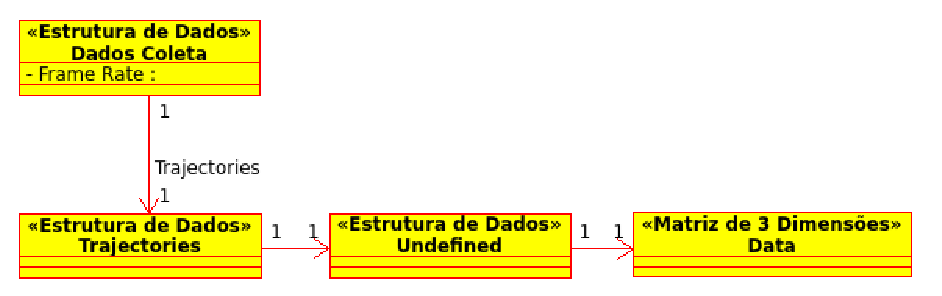
\includegraphics[width=15cm]{figuras/dados_coleta.eps}
	\caption{Dados disponibilizados pelo QTM.}
	\label{dados_coleta}
\end{figure}

São retornados vários dados do QTM, mas os de interesse para o projeto são os que estão na Figura \ref{dados_coleta}. 
O \emph{Frame Rate} é a taxa de coleta dos dados e está em \emph{frames} por segundos. 
A matriz de três dimensões, com dados espaciais dos marcadores passivos de superfície, está disposta da seguinte forma:
\begin{enumerate}
	\item A primeira dimensão tem tamanho variável e representa o número de canais do sistema de coleta, ou seja, cada item representa um marcador;
	\item A segunda dimensão é de tamanho 4 e representa a posição num plano 3D (X, Y, Z) do marcador, mais o erro;
	\item A terceira dimensão é de tamanho variável e representa o número de \emph{frames} coletados numa caminhada específica.
\end{enumerate}

O projeto no qual ocorreu a coleta foi aprovado
pelo Comitê de Ética da Faculdade de Saúde da UnB,
processo N11911/12 (ver Anexo \ref{comite_sec}).

\section[DELIMITAÇÃO DO ESTUDO]{DELIMITAÇÃO DO ESTUDO}

Este trabalho tem como foco estabelecer uma metodologia de desenvolvimento inicial a um sistema de análise e simulação de marcha. 
Ele não busca ser extensivo o suficiente para criar um produto pronto para o mercado, mas pretende, através da implementação de funcionalidades reais, estabelecer uma arquitetura mínima e funcional que sirva de base para a construção do sistema. 
Como consequência, o projeto também integra os principais componentes desta arquitetura, por exemplo, o serviço de banco de documentos, com a \emph{Application Program Interface} (API) \emph{web}.
Um software como este, robusto o suficiente para ser viável no mercado, seria muito caro. 


\section[VISÃO]{VISÃO} 
Apesar deste trabalho ter um objetivo específico e delimitado, dele nasce um projeto maior, cuja visão é o desenvolvimento de um software como serviço para análise e simulação de marcha, utilizando o estado da arte em técnicas para este fim. 
O software deve ser construído utilizando-se métodos ágeis e terá uma arquitetura adaptável que permita evolução contínua.

A estratégia é lançar a versão inicial do software como projeto de código livre, conseguir parceiros e procurar um modelo de negócio sustentável para mantê-lo.

\section[MODELO DE GESTÃO]{MODELO DE GESTÃO}
O software terá um modelo de gestão baseado no método \emph{SCRUM}, como definido em \ref{scrum_sec}.
O método não é adotado na plenitude, sendo adaptado segundo as limitações de recursos do projeto.

Nesta fase inicial, o processo conta com um desenvolvedor, que também assume o papel de \emph{scrum master}, e um \emph{product owner}. 
Devido ao tamanho reduzido da equipe e da localização distinta dos membros, não há \emph{daily scrum}, mas problemas de trabalho cotidianos são resolvidos por telefone, \emph{email} ou mensagens instantâneas. 

O princípio de \emph{time boxing} é mantido. Ficou definido que o \emph{sprint} consiste do prazo de duas semanas. Ao final do \emph{sprint} uma reunião em duas fases é realizada. A primeira fase consiste na revisão do \emph{sprint} anterior. Já a segunda fase é o planejamento do próximo \emph{sprint}.

Um \emph{backlog} de produto é mantido. Na reunião de final de \emph{sprint} é criado um \emph{backlog} de \emph{sprint}. 
Os itens de \emph{backlog} são mantidos na forma de estórias de usuários, conforme \ref{user_stories_sec}.
Na Figura \ref{scrum_projeto} é apresentada a visão geral do processo.

\begin{figure}[ht]
	\centering
	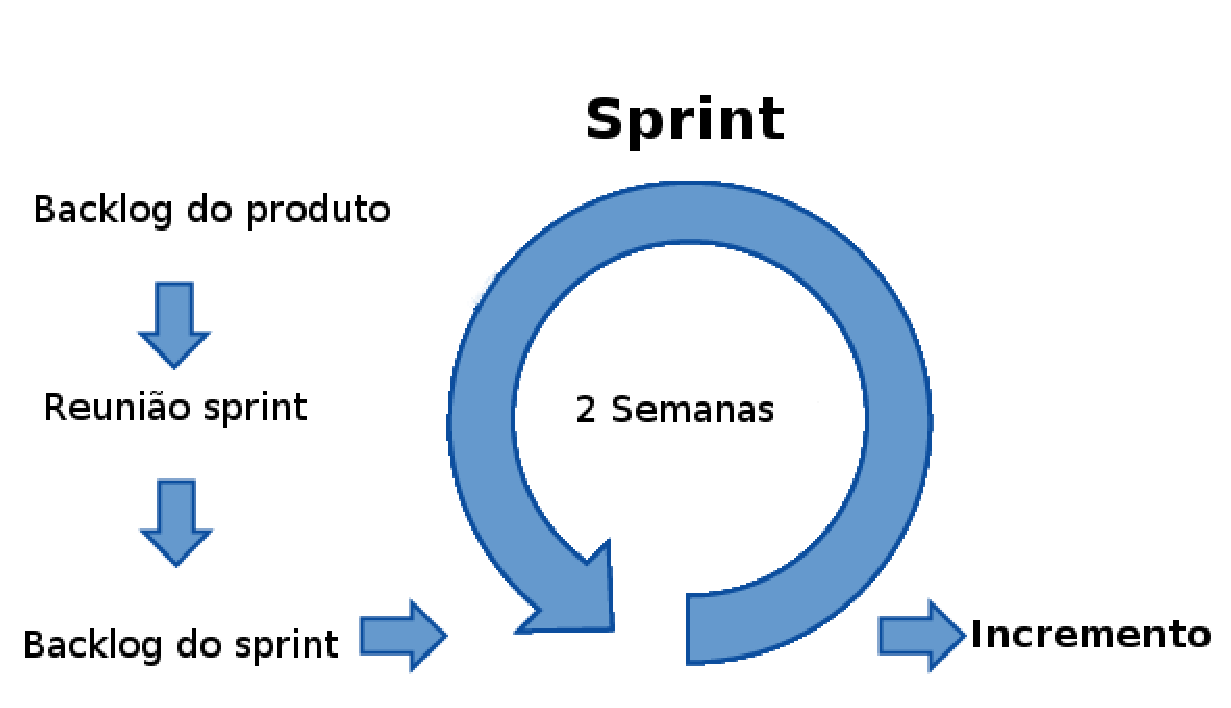
\includegraphics[width=15cm]{figuras/scrum_projeto.eps}
	\caption{Processo de desenvolvimento.}
	\label{scrum_projeto}
\end{figure}






\section[MODELO DE ARQUITETURA]{MODELO DE ARQUITETURA}

O modelo de arquitetura no seu nível mais elevado, pode ser visto como um modelo de três camadas, conforme a Figura \ref{camadas_arquitetura}.
\begin{figure}[ht]
	\centering
	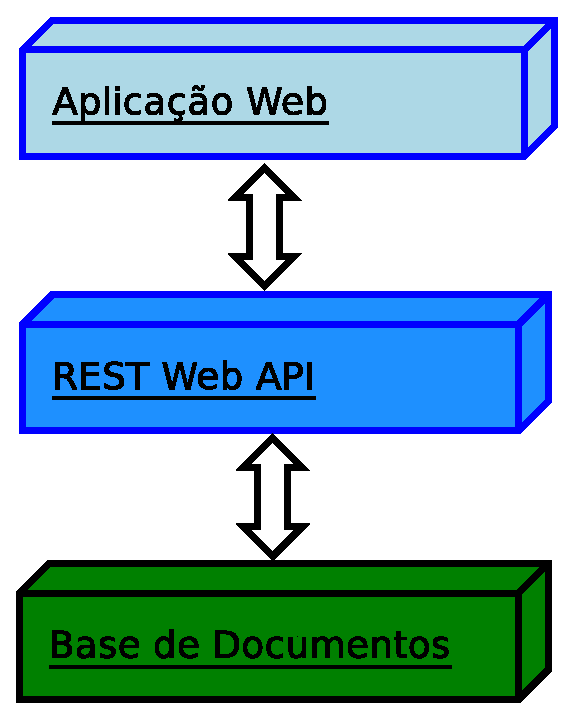
\includegraphics[width=7cm]{figuras/camadas.eps}
	\caption{Camadas arquiteturais.}
	\label{camadas_arquitetura}
\end{figure}

A camada \emph{web} é responsável pela interação com o usuário. 
A camada \emph{Web API} é responsável pela lógica de negócio. 
A camada de base de documentos é responsável pela persistência dos dados da aplicação.


\subsection[CAMADA DE APLICAÇÃO WEB] {CAMADA DE APLICAÇÃO WEB}
Esta camada foi projetada para rodar em \emph{browsers} que suportam \emph{HTML} 5. 
Ela é desenvolvida usando-se \emph{Javascript}, \emph{CSS} e \emph{HTML}. 
Além disso, adotou-se o \emph{framework} de desenvolvimento \emph{web} \emph{AngularJS}, ver \ref{angularjs}. 

Como o projeto não possuía recursos adequados a criação de uma equipe de desenvolvimento \emph{web} completa, afim de se minimizar os problemas com \emph{design web}, optou-se por usar a biblioteca \emph{angular-material}, ver \ref{angular_material}. 

A Figura \ref{material_amostra}, mostra um exemplo de uma tela criada com as diretivas do angular-material. Note que todo o \emph{look and feel} da tela é determinado pelo comportamento padrão da biblioteca.

\begin{figure}[H]
	\centering
	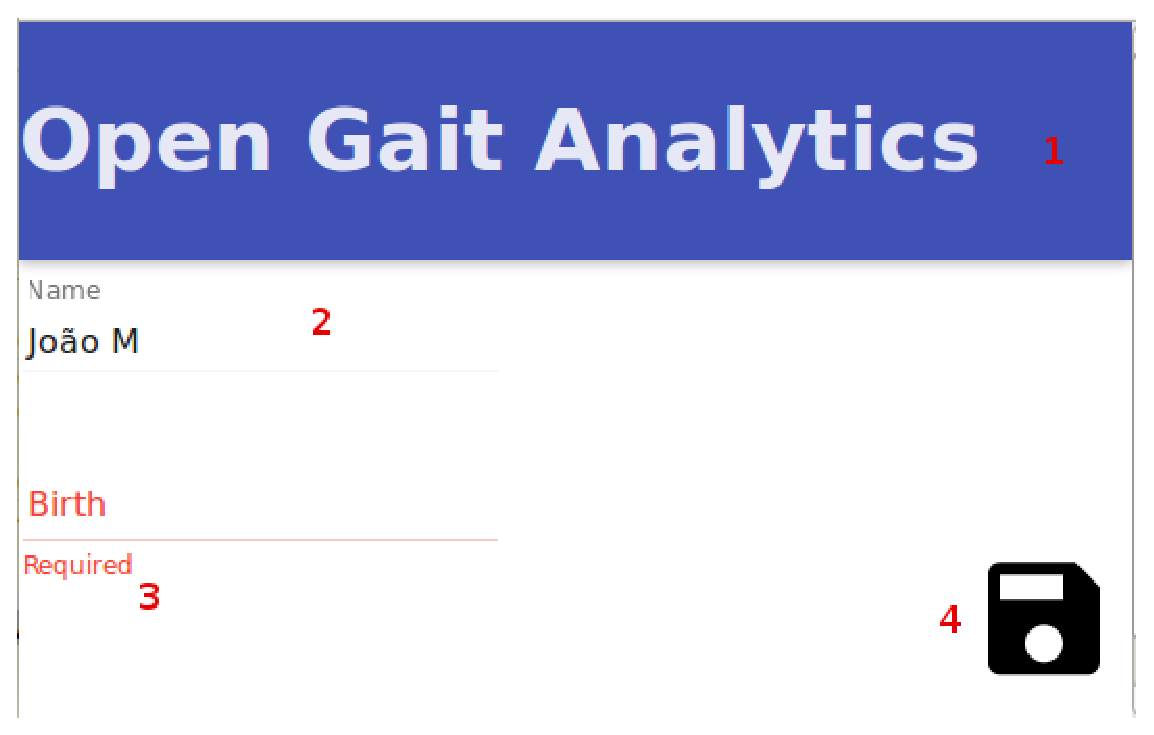
\includegraphics[width=9cm]{figuras/material_amostra.eps}
	\caption[Exemplo de uma tela criada com \emph{angular-material}.]{Exemplo de uma tela criada com \emph{angular-material}. 1) Diretiva \emph{md-toolbar}; 2) Diretiva \emph{md-input-container}; 3) Diretiva \emph{ng-messages} em conjunto com a \emph{md-input-container}; 4) Diretiva \emph{md-button}.}
	\label{material_amostra}
\end{figure}

\textbf{ORGANIZAÇÃO DO CÓDIGO FONTE}

\noindent
A criação de um ambiente de desenvolvimento \emph{web}, para um software de média para grande complexidade, não é uma tarefa trivial de ser resolvida.
É necessário criar padrões de organização de arquivos, configurar e instalar pacotes de software para desenvolvimento, testes, implantação, construção de \emph{builds}, entre outros.
Para facilitar esta tarefa, optou-se em utilizar o projeto \emph{angular-seed}, ver \ref{angular_seed}.
A ideia deste projeto é servir de esqueleto de projetos \emph{web} que utilizam o \emph{framework} \emph{AngularJS}.
Para usar este projeto, basta cloná-lo diretamente do seu repositório \emph{git} no \emph{site} github.com, conforme o comando abaixo.
\lstset{language=bash}
\begin{lstlisting}[frame=single]
git clone https://github.com/angular/angular-seed.git
\end{lstlisting}

\textbf{VISÃO ARQUITETURAL DA CAMADA \emph{WEB}}


\noindent
A Figura \ref{camda_web} mostra o funcionamento e os padrões mínimos a serem seguidos para implementação da camada \emph{web}.

\begin{figure}[H]
	\centering
	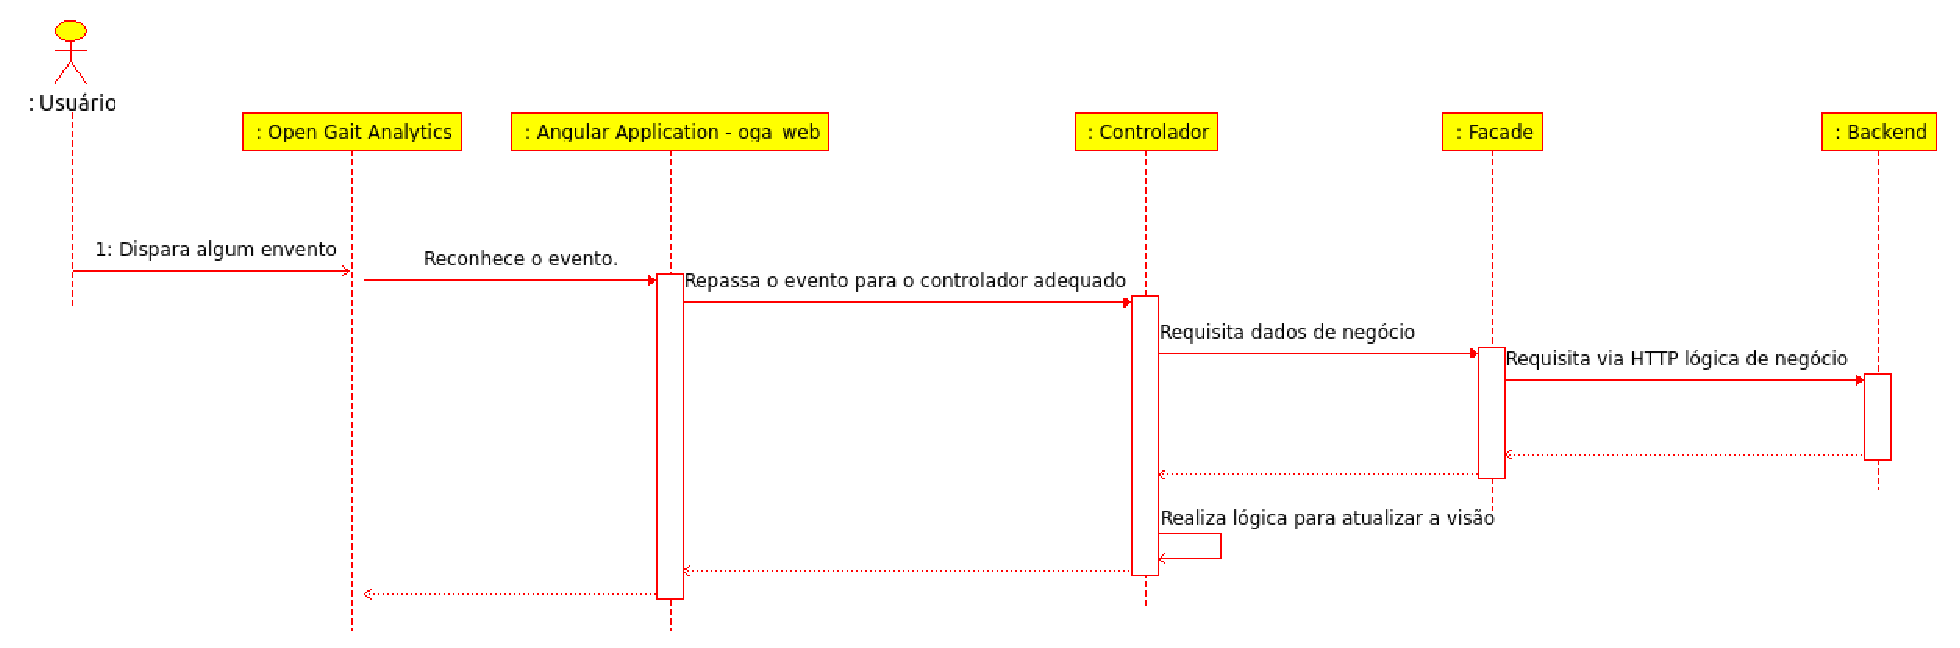
\includegraphics[width=17cm]{figuras/camada_web.eps}
	\caption{Camada \emph{web}.}
	\label{camda_web}
\end{figure}

Este esquema funciona da seguinte forma: O usuário usando seu \emph{browser}, acessa o \emph{site} do software. 
Ao realizar qualquer evento na aplicação, por exemplo, clicar num botão, ou selecionar um item em uma lista de seleção, a aplicação \emph{angularjs} detecta o evento e seleciona um componente de software chamado controlador. 
Existem vários destes controladores no sistema, cada evento do usuário é redirecionado para um que seja adequado.
No controlador é onde grande parte da programação acontece. 
Ele é associado a um \emph{template HTML}. 
Este template funciona como componente de apresentação para o usuário, e é o que o controlador manipula para mostrar informações ao usuário.
Quando o controlador precisa executar lógica de negócio, ou requisitar dados persistidos, ele deve chamar um componente do tipo \emph{Facade}. 
A aplicação \emph{web} roda no \emph{browser} do usuário e não persiste dados nem executa lógica de negócio. 
Este é um estilo arquitetural escolhido para o projeto.
A \emph{Facade} é um \emph{proxy} que se comunica com um \emph{backend} via HTTP no estilo \emph{REST} de comunicação via \emph{web}.

A Figura \ref{web_components}, mostra um exemplo de componentes escritos em \emph{JavaScript} respondendo a um evento disparado pelo usuário. 
Este evento poderia ser oriundo de um clique num botão ou na chamada de uma \emph{URL} específica. 
Depois de reconhecido o evento, no caso um pedido para ver a lista de pacientes, o componente \emph{PatientesCtrl} e o \emph{template patients.html} são carregado pelo \emph{framework AngularJS}. 
Neste momento o \emph{framework} acessa o componente \emph{PatientsFacade} através do seu método \emph{getPatients}. 
Este método invoca o método \emph{get} do componente \emph{\$HTTP} que faz parte do \emph{framework}.
Uma requisição é feita para o \emph{backend}, que retorna os dados no formato \emph{JSON}.
Finalmente, o \emph{framework} detecta a resposta e atualiza a tela para o usuário.

\begin{figure}[H]
	\centering
	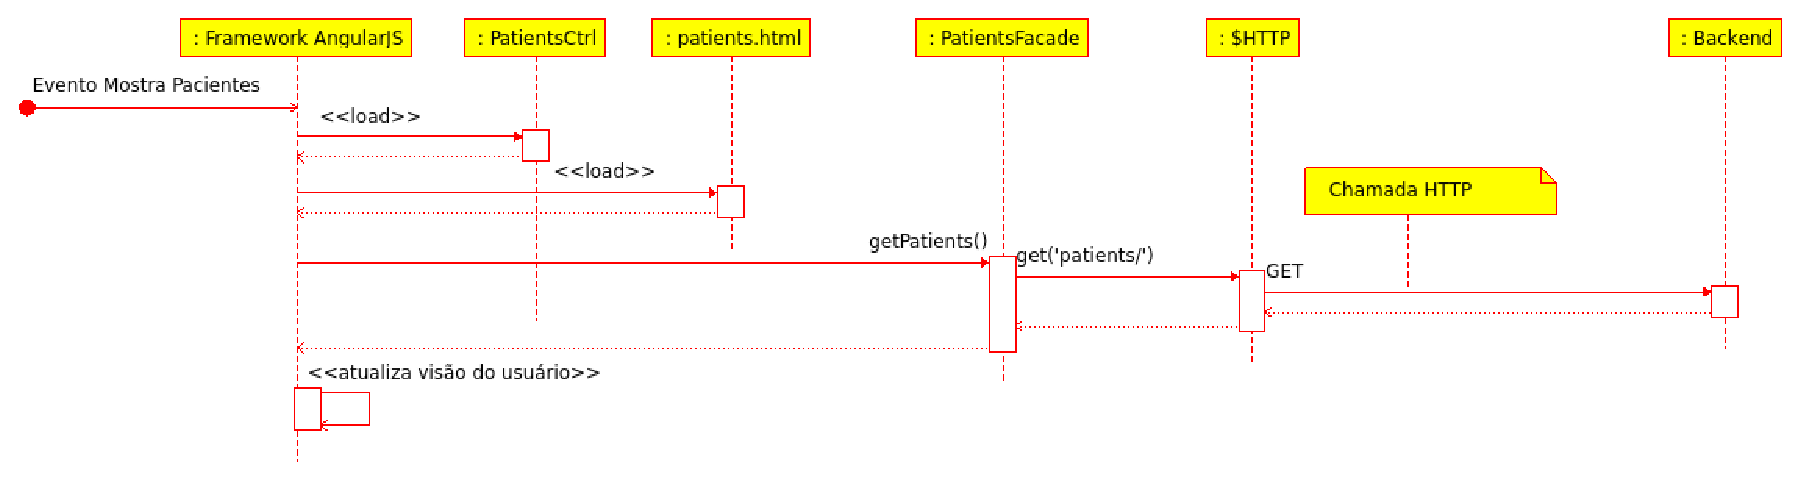
\includegraphics[width=17cm]{figuras/web_componentes.eps}
	\caption{Exemplo de componentes da camada \emph{web} funcionando juntos.}
	\label{web_components}
\end{figure}


\subsection{CAMADA \emph{REST WEB API}}

Esta é a camada responsável por expor toda a lógica de negócio e acesso a dados persistidos. Escolheu-se que esta camada fornece suas funções via \emph{web API} no estilo REST.
Uma das vantagens desta escolha é o alto desacoplamento, entre camada \emph{web} e lógica de negócio. 
Além disso, pode-se integrar mais facilmente a aplicação com outras, já que a lógica de negócio é toda exposta como \emph{API web}. 
Veja a seção \ref{servicos_rest} para um melhor entendimento deste estilo \emph{REST}.

\textbf{ORGANIZAÇÃO DO CÓDIGO FONTE}

\noindent
A Figura \ref{dir_api} mostra a configuração básica dos arquivos e diretórios da aplicação.

\begin{figure}[ht]
	\centering
	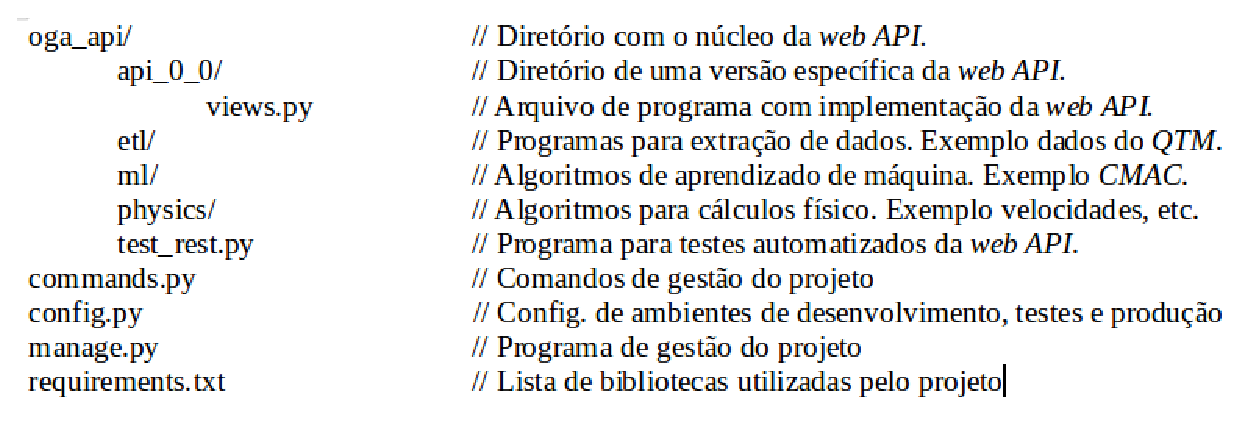
\includegraphics[width=15cm]{figuras/dir_api.eps}
	\caption{Organização do arquivos e diretórios da camada \emph{web API}.}
	\label{dir_api}
\end{figure}

A linguagem de programação \emph{Python} foi escolhida para implementar esta camada. Vários foram os motivos: a biblioteca \emph{Flask} para implementar a \emph{web API}, a biblioteca \emph{NumPy}, que é excelente para cálculos, comparável ao Matlab, a biblioteca \emph{Matplotlib} para criação de gráficos científicos, a baixa curva de aprendizado da linguagem, sua fama com desenvolvedores ao redor do mundo.

Para diminuir os problemas de ambientes, oriundos de um projeto complexo como este, optou-se por utilizar o programa \emph{virtualenv}. Este programa cria um ambiente \emph{python} virtual, baseado num arquivo de configuração. Isso faz com que todos os desenvolvedores envolvidos no projeto, possuam ambientes muito semelhantes.
Ao se clonar o projeto basta entrar no diretório da API e digitar o comando:
\lstset{language=bash}
\begin{lstlisting}[frame=single]
virtualenv env
\end{lstlisting}

Este comando irá criar uma diretório chamado \emph{env}. Para poder ativar o ambiente virtual é necessário o comado no unix:
\lstset{language=bash}
\begin{lstlisting}[frame=single]
. env/bin/activate
\end{lstlisting}

As bibliotecas necessárias a execução da aplicação estão listadas no arquivo \emph{requirements.txt}. Para instalá-las no novo ambiente virtual é necessário o comando:
\lstset{language=bash}
\begin{lstlisting}[frame=single]
pip install -r requirements.txt
\end{lstlisting}

Neste ponto, o código já pode ser editado e executado. Para facilitar um pouco as coisas, foi criado o programa \emph{manage.py}. Para rodar um servidor \emph{web} local respondendo na porta 5000, com fins de desenvolvimento, basta digitar o comando:
\lstset{language=bash}
\begin{lstlisting}[frame=single]
python manage.py runserver
\end{lstlisting}

Já para executar testes automatizados:
\lstset{language=bash}
\begin{lstlisting}[frame=single]
python manage.py test
\end{lstlisting}

Vale lembrar que o servidor \emph{MongoDB}, deve estar configurado, rodando e suas configurações editadas no arquivo \emph{config.py}.


\textbf{VISÃO ARQUITETURAL DA CAMADA \emph{REST WEB API}} 

\noindent
A Figura \ref{camada_api} mostra um \emph{blueprint} de como funciona e como deve ser desenvolvida esta camada.
\begin{figure}[ht]
	\centering
	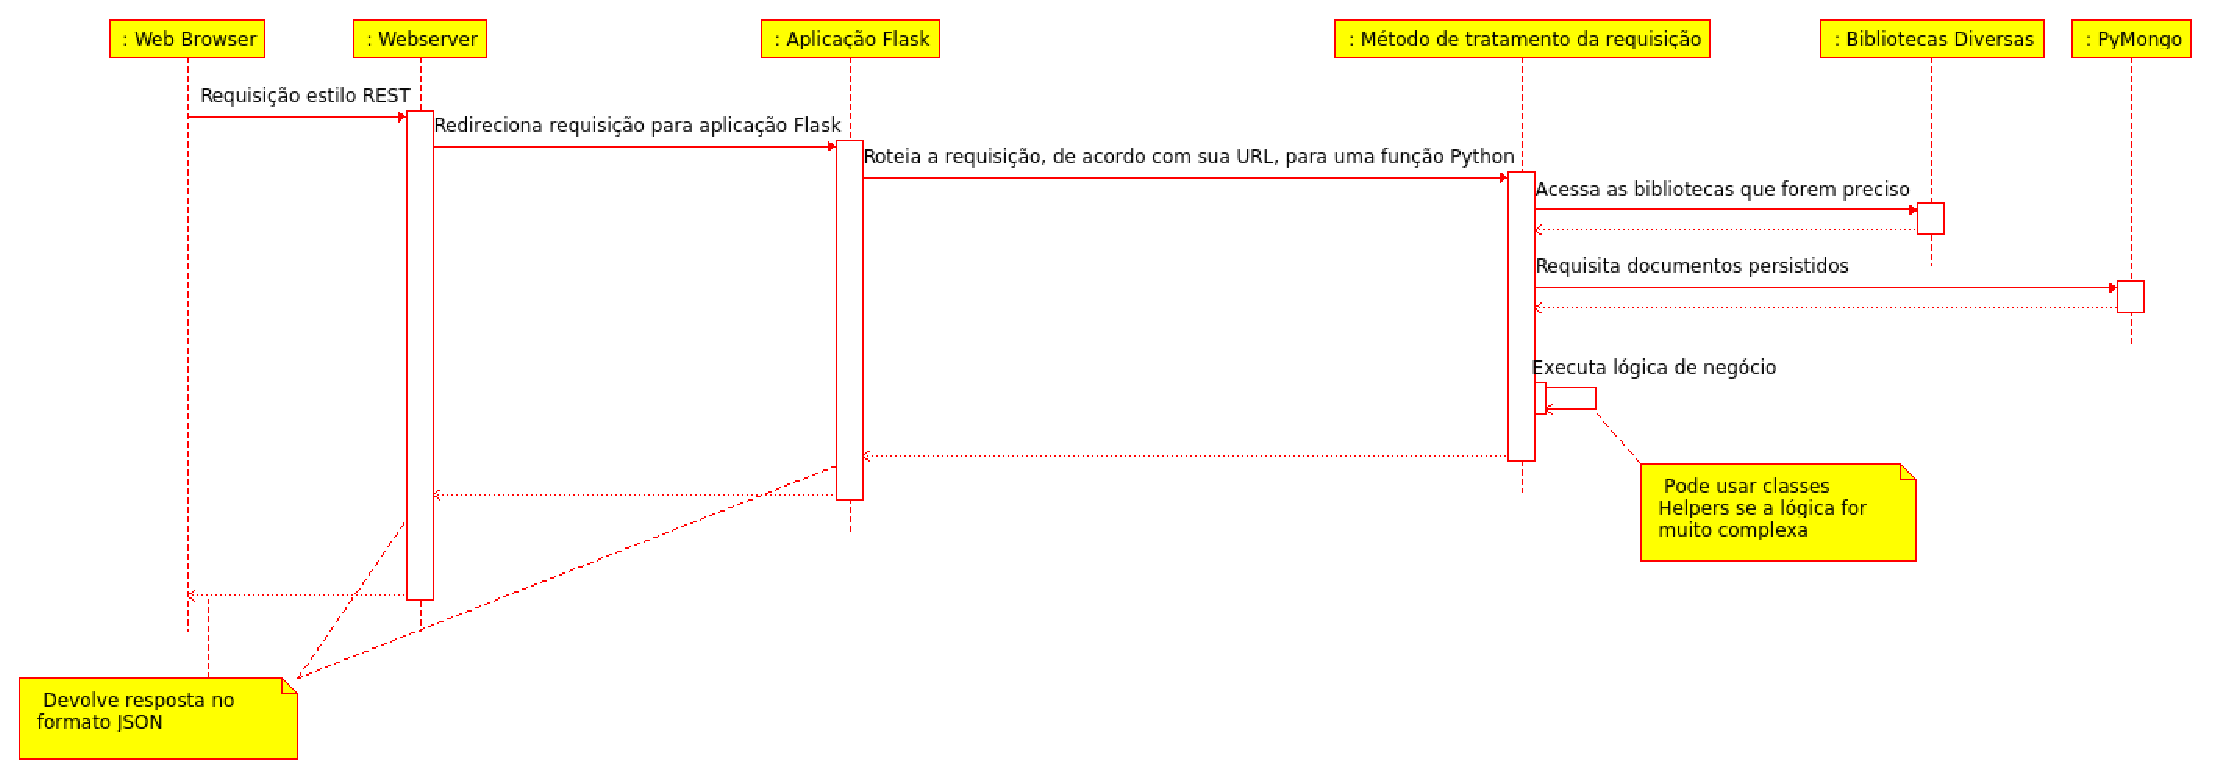
\includegraphics[width=15cm]{figuras/camada_api.eps}
	\caption{Camada \emph{REST WEB API}.}
	\label{camada_api}
\end{figure}

Tudo começa quando um \emph{browser web} faz uma requisição do tipo \emph{HTTP} a um servidor \emph{web}. 
O servidor \emph{web} identifica se a requisição é para a aplicação \emph{flask} do sistema em questão. 
Se for, esta requisição é repassada para a aplicação \emph{flask}. 
Agora as coisas começam a ficar mais interessantes. 
A aplicação \emph{flask} analisa a \emph{URL} da requisição, verifica o método da requisição e repassa os dados da requisição, num formato amigável ao \emph{python}, para uma função \emph{python}. 
Por padrão os parâmetros das requisições via método \emph{``GET"} são repassadas ao \emph{python} como \emph{string}. 
Para os demais métodos, padronizou-se receber o \emph{payload} da requisição \emph{HTTP}, como objetos JSON, que são facilmente convertidos para dicionários \emph{python}.

São nas funções \emph{python}, que tratam as requisições, que a lógica de negócio é executada. 
Aqui bibliotecas como a \emph{NumPy} podem ser chamadas, ou mesmo bibliotecas criadas pelos desenvolvedores da aplicação. 
É a partir deste ponto que dados podem ser acessados do banco de documentos pela biblioteca \emph{PyMongo}. 
Ao final da execução uma resposta é gerada no formato \emph{JSON} para que seja consumida pela camada \emph{web}.

A Figura \ref{webapi_componentes}, mostra um exemplo de componentes escritos em \emph{Python}, tratando uma requisição \emph{HTTP}, no caso uma chamada a \emph{URL http://<<myurl>>/patient}.
Depois que o servidor \emph{web} repassou a requisição para a aplicação que usa o \emph{framework Flask}, o \emph{framework} executa sua rotina de roteamento e descobre qual função \emph{Python}, contida no componente \emph{views},  deve ser executada, no caso a função \emph{get\_patients}.
Esta função acessa um objeto do tipo \emph{DataBase}, pertencente a biblioteca \emph{PyMongo}, e executa o método \emph{find} da coleção \emph{patients} pertencente ao \emph{DataBase}.
O resultado desta chamada são os dados contidos no banco de dados retornados no formato \emph{BSON}.
O componente \emph{json\_util}, da biblioteca \emph{PyMongo}, tem seu método \emph{dumps} chamado.
Este método converte os dados de \emph{BSON} para \emph{JSON}.
Finalmente, o \emph{framework Flask} responde a requisição.


\begin{figure}[ht]
	\centering
	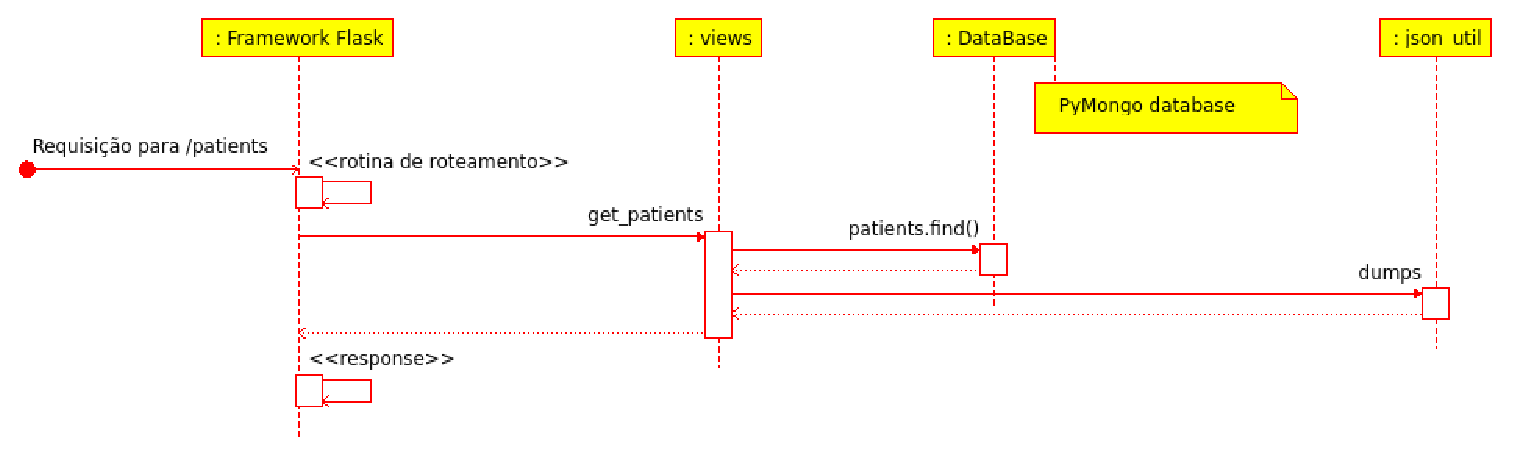
\includegraphics[width=17cm]{figuras/webapi_componentes.eps}
	\caption{Exemplo de requisição sendo tratada pela \emph{web api}.}
	\label{webapi_componentes}
\end{figure}

\subsection {CAMADA DE BASE DE DOCUMENTOS}

Para esta camada foi escolhido o banco de documentos \emph{MongoDB}, ver a seção \ref{mongodb_sec}. 
Há várias vantagens no uso desta tecnologia, mas a determinante foi a facilidade de uso e criação de estruturas de dados. 
No início do projeto, foi usado um banco de dados relacional e um \emph{framework} de mapeamento objeto-relacional. 
Devido a natureza altamente complexa dos dados, dados espaciais provindos de marcadores de superfície capturados por câmeras, eles são multidimensionais também. 
Sem dúvida isto ajudou a tornar possível criar esta primeira versão do software em tão pouco tempo.

A estrutura do banco da aplicação é mostrada na Figura \ref{mongo_oga}. 
O banco é composto por duas coleções: os dados dos pacientes na coleção \emph{patients} e os dados recuperados do \emph{QTM} \emph{positionals\_data}.

\begin{figure}[H]
	\centering
	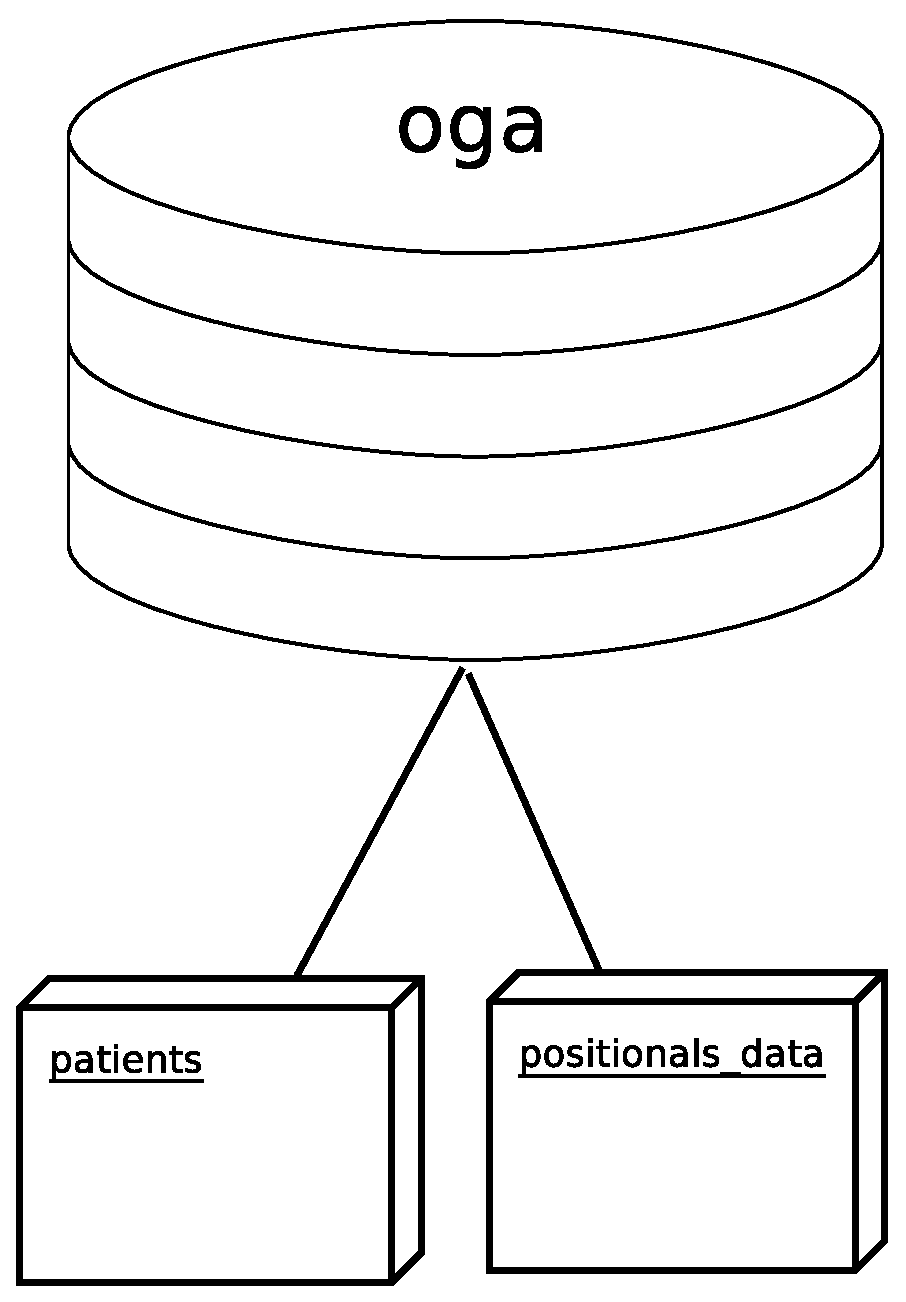
\includegraphics[width=5cm]{figuras/mongo_oga.eps}
	\caption{Banco de documentos da aplicação.}
	\label{mongo_oga}
\end{figure}

A Figura \ref{listagem2}  mostra um exemplo de documento da coleção \emph{patients}.
Já a Figura \ref{listagem3}  mostra um exemplo de documento da coleção \emph{positionals\_data}.

\begin{figure}[H]
	\centering
	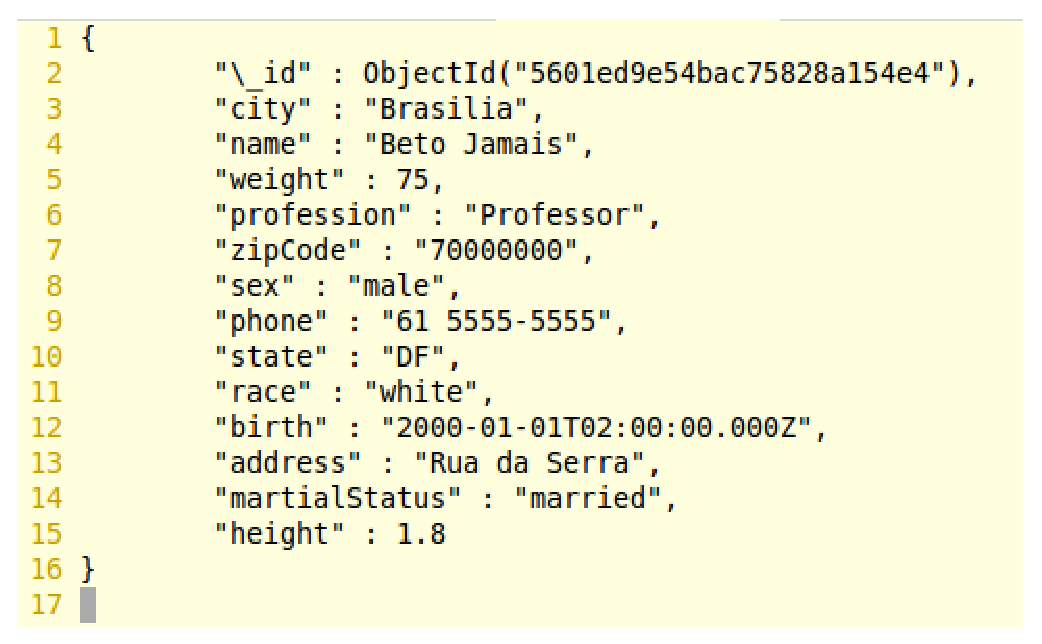
\includegraphics[width=10cm]{figuras/listagem2.eps}
	\caption{Documento da coleção \emph{patients}.}
	\label{listagem2}
\end{figure}

\begin{figure}[H]
	\centering
	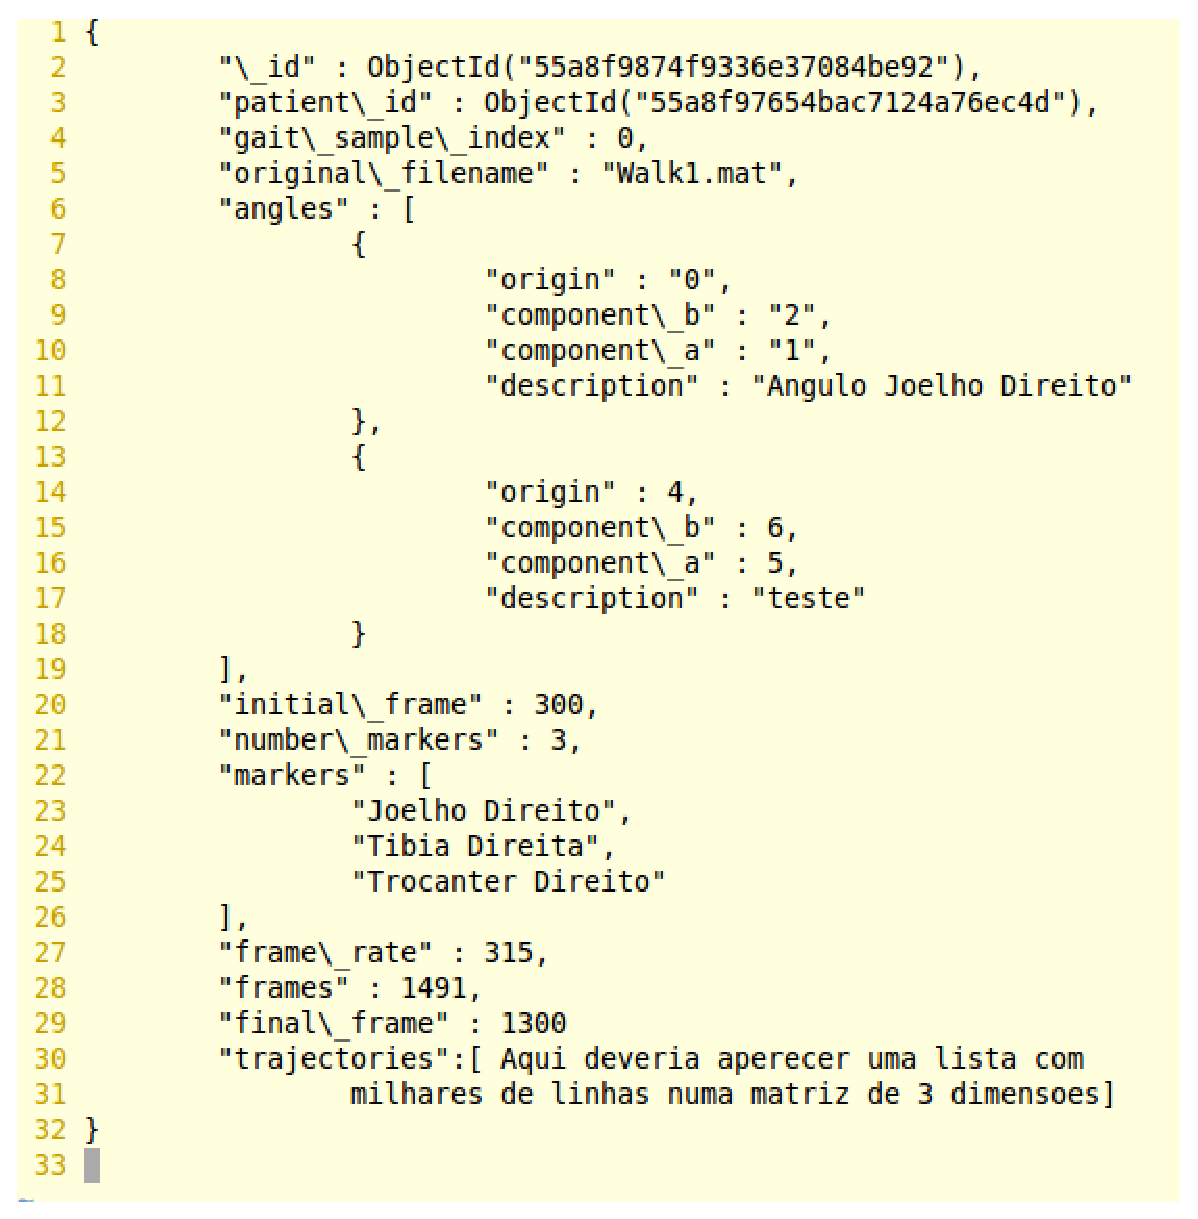
\includegraphics[width=10cm]{figuras/listagem3.eps}
	\caption{Documento da coleção \emph{positionals\_data}.}
	\label{listagem3}
\end{figure}




\begin{comment}
\section[FASES ESTUDO]{FASES DO ESTUDO}
\subsection[Coleta dos Dados]{\textbf{Coleta dos Dados}}
Os dados para o treinamento da RNA CMAC são dados cinemáticos, capturados através de \emph{motion capture}, utilizando-se de várias câmeras \emph{Qualisys Oqus MRI}, com marcadores passivos e pacote de software \emph(QTM 3.2) da \emph{Qualisys}. 
O sistema utilizado suporta até 74 canais, ou marcadores simultâneos.

O projeto no qual ocorreu a coleta foi aprovado pelo Comitê de Ética da Faculdade de Saúde da UnB, processo N11911/12 (ver Anexo \ref{anexo1}).

A Figura \ref{coleta_dados} mostra o processo para coleta de dados.

\begin{figure}[ht]
 \centering
 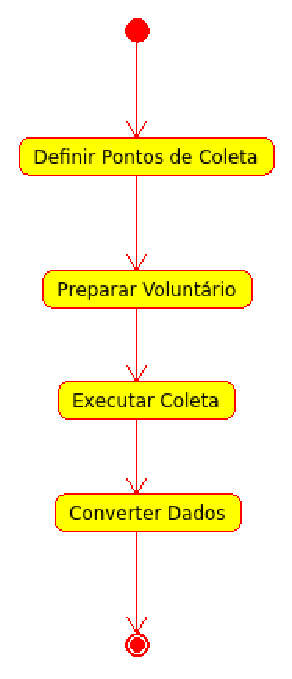
\includegraphics[width=4cm]{figuras/coleta_dados.eps}
 \caption{Fluxo de coleta de dados.}
 \label{coleta_dados}
\end{figure}

Primeiro deve-se definir o voluntário da coleta e determinar o dia para este processo. 
Além disso, também é necessário definir quais os pontos no corpo do voluntário devem ser mapeados. 
Também se devem distribuir os marcadores em várias posições ao longo das pernas. 
Como só a flexão e a extensão dos joelhos interessam para este trabalho, utilizam-se somente marcadores nas tíbias, joelhos e trocânteres das duas pernas.

O próximo passo se refere ao voluntário, isto é, ele deve repetir um ciclo de marcha confortável de aproximadamente 5 segundos, por 5 vezes na frente das câmeras.

Quanto aos dados, estes devem ser convertidos para formato adequado à linguagem \emph{Octave}, que é a mesma opção para converter para o \emph{MATLAB}. Esta opção é própria do \emph{QTM}. 
Além da conversão é necessário definir o nome de cada item na matriz de dados coletados. 
Cada coluna desta matriz representa um marcador, são estes pontos que devem ser nomeados. 
Por exemplo, coluna 1 igual ao trocânter direito. 
O número que o QTM atribui internamente ao marcador é a posição do marcador na matriz. 
Este número é chamado dentro do QTM de canal. 
Os dados trazem variáveis espaciais e o erro, com respeito à posição (X, Y, Z) dos marcadores.

A disposição que os dados obtidos neste processo se apresentam, é mostrado na Figura \ref{dados_qtm}.

\begin{figure}[ht]
 \centering
 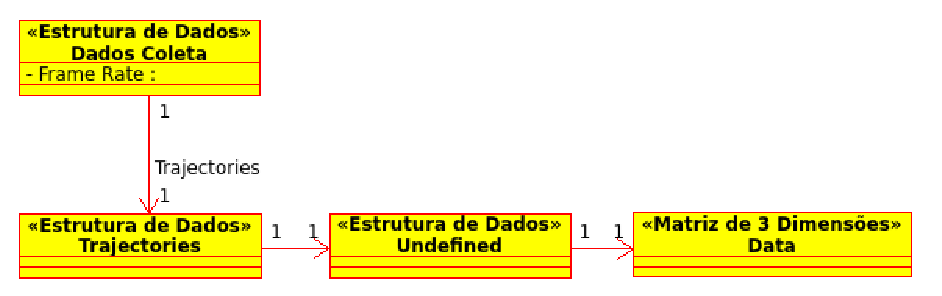
\includegraphics[width=15cm]{figuras/dados_qtm.eps}
 \caption{Dados disponibilizados pelo QTM.}
 \label{dados_qtm}
\end{figure}

Os dados que interessam são o \emph{Frame Rate} e o \emph{Data}.
São retornados vários dados, mas os de interesse para o projeto são os que estão na Figura \ref{dados_qtm}. 
O \emph{Frame Rate} é a taxa de coleta dos dados e está em segundos. 
A matriz de 3 dimensões está disposta da seguinte forma:
\begin{enumerate}
	\item A primeira dimensão é 74 e representa o número de canais do sistema de coleta;
	\item A segunda dimensão é 4 e representa a posição num plano 3D (X, Y, Z) do marcador, mais o erro;
	\item A terceira dimensão é número de frames coletados numa caminhada específica. Este número é variável.
\end{enumerate}



\subsection[Extração e transformação dos dados]{\textbf{Extração e transformação dos dados}}
Com os dados necessários disponibilizados no formato adequado é possível fazer os cálculos de angulações, velocidades angulares e acelerações angulares dos joelhos. Os casos de uso para esta fase são:
\begin{figure}[ht]
	\centering
	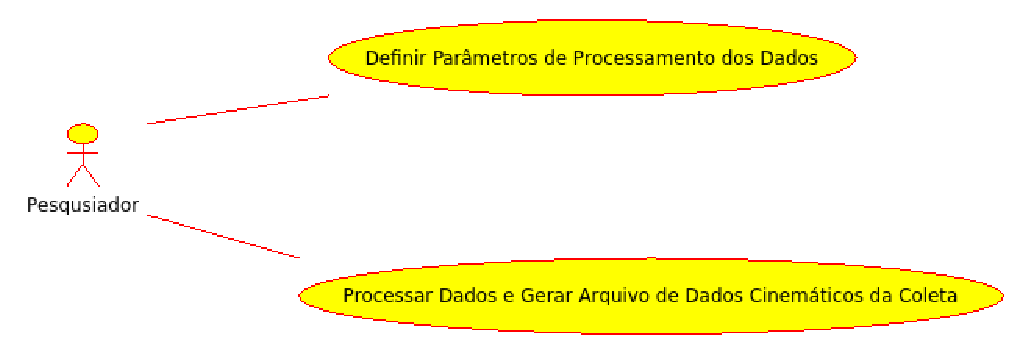
\includegraphics[width=15cm]{figuras/extracao_coleta.eps}
	\caption{Caso de uso para extração e transformação de dados}
	\label{extracao_coleta}
\end{figure}

O caso de uso Definir Parâmetros de Processamento dos Dados, definido na Figura \ref{extracao_coleta}, consiste em se definir os dados necessários para que depois seja possível processar os dados coletados. 
Estes dados são os definidos na Figura \ref{estrutura_dados}. 
O valor dos 6 primeiros atributos da estrutura de dados Configuração do Processamento, são os canais usados no QTM para tais marcadores.
\begin{figure}[ht]
	\centering
	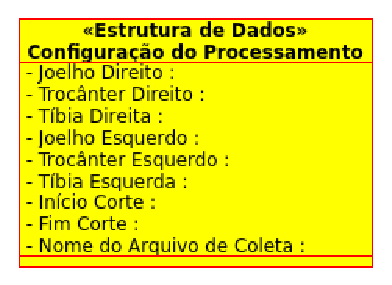
\includegraphics[width=7.5cm]{figuras/estrutura_dados.eps}
	\caption{Dados para processamento da coleta.}
	\label{estrutura_dados}
\end{figure}

O caso de uso Processar Dados e Gerar Arquivos de Dados Cinemáticos, definido na Figura \ref{extracao_coleta}, da coleta deve obedecer o processo da Figura \ref{tratamento_dados}.
\begin{figure}[ht]
	\centering
	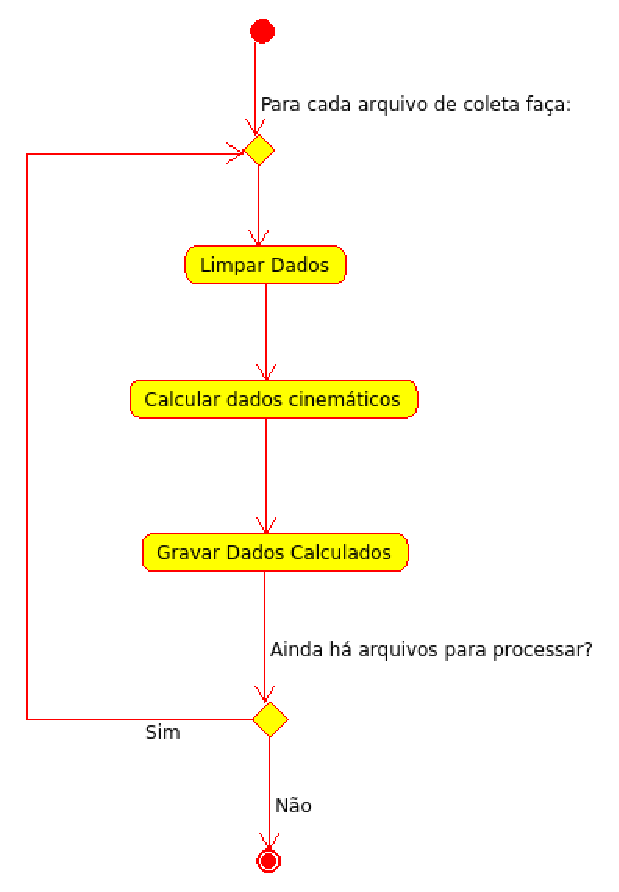
\includegraphics[width=10cm]{figuras/tratamento_dados.eps}
	\caption{Processo de tratamento dos dados.}
	\label{tratamento_dados}
\end{figure}

A limpeza dos dados consiste em retirar os dados desnecessários, como marcadores não desejados e retirada de frames do início e/ou final de um arquivo de coleta, que não estejam no ciclo de marcha confortável. 

Os cálculos realizados devem ser as velocidades instantâneas, velocidades angulares e acelerações angulares. 
Velocidades instantâneas dos joelhos são calculadas conforme a Equação \ref{velocidade}.
\begin{equation}
	\label{velocidade}
	\vec{\nu} = (\vec{a}-\vec{b})/t 
\end{equation}

A variável $\vec{a}$  é a posição (X, Y, Z) do joelho em uma determinada leitura sequencial dos dados coletados. 
A variável $\vec{b}$ é a próxima posição (X, Y, Z) da sequência. $t$ é o \emph{frame rate} definido nos dados da coleta.

Para o cálculo das angulações dos joelhos, primeiro os marcadores destes devem ser transladados para uma origem, assim é possível se usar a Equação 5 como descrita em \citeonline{Edwards2006}. 
Para tal, usam-se as Equações \ref{trocanter}, \ref{joelho} e \ref{tibia}.
\begin{equation}
	\label{trocanter}
	\vec{t_{r0}} = \vec{t_r} - \vec{j}
\end{equation}
\begin{equation}
	\label{joelho}
	\vec{j_0} = \vec{j} - \vec{j}
\end{equation}
\begin{equation}
	\label{tibia}
	\vec{t_{b0}} = \vec{t_b} - \vec{j}
\end{equation}

$\vec{t_{r0}}$ é o vetor que representa a posição de um trocânter $\vec{t_r}$, transladado para a nova origem.
$\vec{j}$ é vetor da posição do joelho.
$\vec{j_0}$ é a nova origem, que nada mas é que o joelho transladado para a posição $(0,0,0)$. 
$\vec{t_{b0}}$ é a posição da tíbia $\vec{t_b}$ transladada para a origem.
A translação de vetores é documentada em \citeonline{Poole2011}.

Agora que se tem os pontos transladados para uma origem, pode-se usar a Equação \ref{ang_joe} para o cálculo do ângulo $\theta$ do joelho.
\begin{equation}
	\label{ang_joe}
	\theta =
		cos^{-1} 
		\frac
		{
			\vec{t_{r0}} \cdot \vec{t_{b0}}
		}
		{
			\left \| \vec{t_{r0}} \right \|
			\cdot
			\left \| \vec{t_{b0}} \right \|
		}
\end{equation}

O operador $\left \| \right \|$ é o cálculo da distância euclidiana, ou norma. Pode ser calculado, segundo \citeonline{Poole2011}, de acordo com a Equação \ref{norma}. Resumindo, é a raiz quadrada do produto interno de um vetor.
\begin{equation}
	\label{norma}
	\left \| \vec{u} \right \| = \sqrt{\vec{u}\cdot\vec{u}}
\end{equation}

A velocidade angular $\omega$ do joelho é calculada a partir da Equação \ref{vel_ang}.
\begin{equation}
	\label{vel_ang}
	\omega = (\theta_1 - \theta_2) / t
\end{equation}

A variável $\theta_1$ é o ângulo de um joelho num determinado frame. A variável $\theta_2$ é exatamente o ângulo do próximo frame. A variável $t$ é o \emph{frame rate}, oriundo dos dados da coleta.


A última etapa deste processo é a gravação dos dados para que possam ser usados pela RNA CMAC. 
Estes dados devem ser gravados num arquivo em formato texto. 
As linhas neste arquivo equivalem aos \emph{frames}. 
Cada coluna equivale às informações, na ordem em que aparecem, da estrutura de dados descrita na Figura \ref{dados_cinematicos}. 
\begin{figure}[ht]
	\centering
	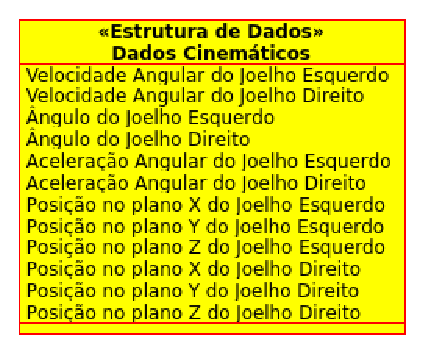
\includegraphics[width=7.5cm]{figuras/dados_cinematicos.eps}
	\caption{Dados Cinemáticos da Marcha}
	\label{dados_cinematicos}
\end{figure}

\subsection[Construção de uma RNA CMAC]{\textbf{Construção}}
\subsubsection{Modelo Geral}

A RNA CMAC proposta para este trabalho é resumida na Figura \ref{camac_resumida}.

\begin{figure}[ht]
	\centering
	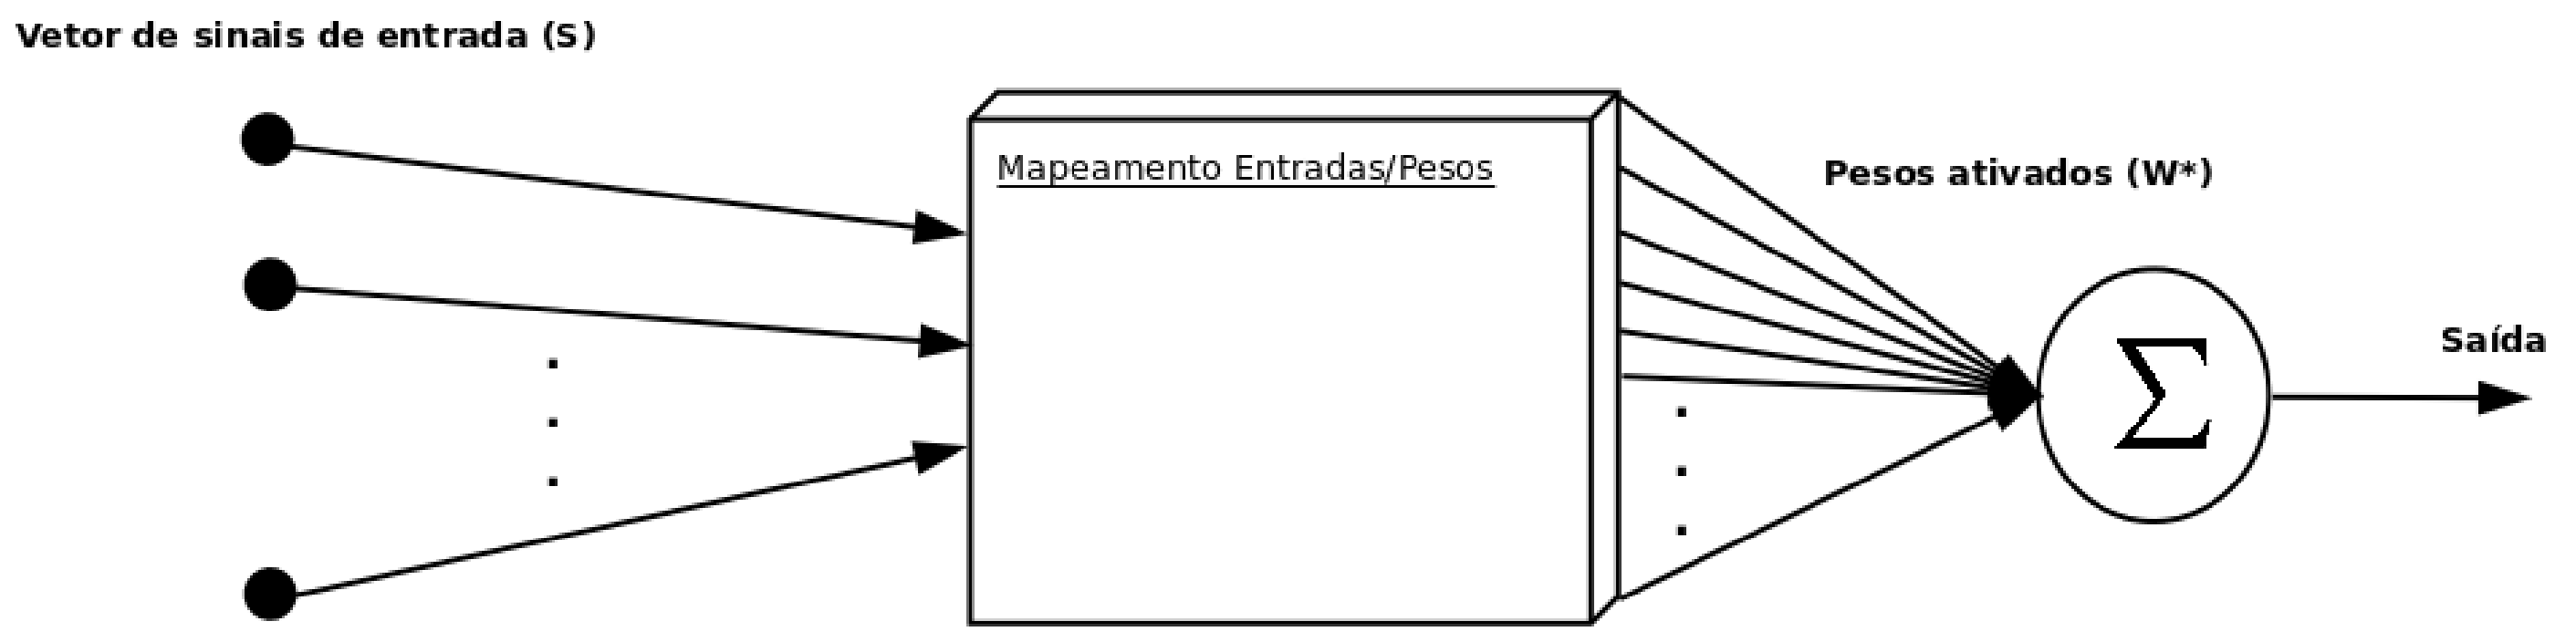
\includegraphics[width=15cm]{figuras/cmac_resumida.eps}
	\caption{CMAC resumida.}
	\label{camac_resumida}
\end{figure}

A variável $S$ é o vetor de sinais de entrada. 
Esses sinais são passados para um processo de mapeamento entre a entrada e um conjunto de pesos. 
Depois apenas os pesos ativados participam da somatória que é o sinal de saída. 

Para se calcular a saída da rede, primeiramente define-se o número de pesos $NW*$ a serem ativados.

O segundo passo é definir os possíveis valores para cada item do vetor de entradas $S$. A isto chama-se quantização. Por exemplo, se o primeiro item $s1$ de $S$ aceita valores entre $-1$ até $1$ e se quer $5$ valores possíveis, quantiza-se $s1$ conforme a Figura \ref{quantizacao}.
\begin{figure}[ht]
	\centering
	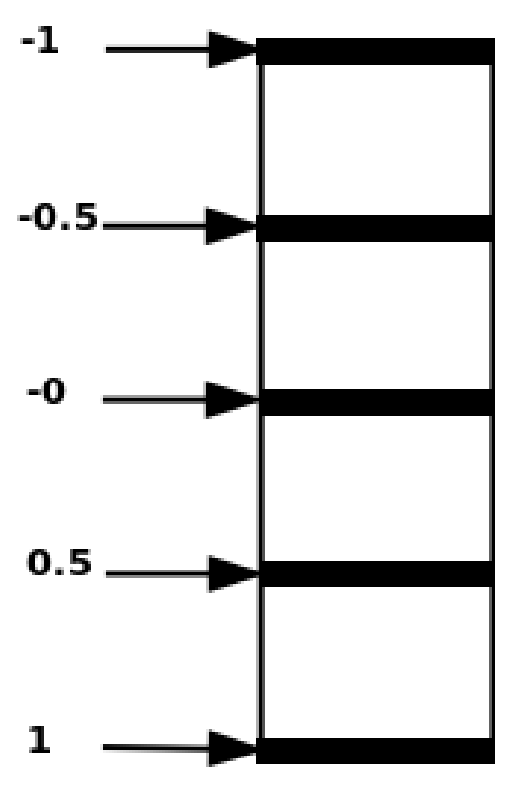
\includegraphics[width=5cm]{figuras/quatizacao.eps}
	\caption{Quantização de $s1$}
	\label{quantizacao}
\end{figure}

Isto significa que quaisquer que sejam os valores de $s1$ os mesmos devem ser convertidos para $-1$, $-0,5$, $0$, $0,5$ e $1$. 
Por exemplo, se o valor de s1 for $0,75$, será convertido para o valor $1$, se for $-0,75$ será o valor $0$ e se for $0,25$ será o valor $0,5$. À discretização dá-se o nome de resolução da CMAC.

O próximo passo é criar uma tabela para cada um dos sinais discretizados de entrada do vetor $S$.
Supondo que o vetor $S$ possui 2 sinais de entrada $s1$ e $s2$ e um número de ativações $NW*$ igual a 3, cria-se Tabela \ref{map_s1} e a Tabela \ref{map_s2}. 
Para facilitar o entendimento, irá se considerar os valores de $s1$ iguais aos inteiros de 1 até 6 e os valores de s2 iguais aos inteiros de 1 até 4.
\begin{table}[htb]
	\IBGEtab{%
		\caption{Mapeamento de $s1$}%
		\label{map_s1}
	}
	{%
		\begin{tabular}{cc}
			\toprule
			\textbf{Valores de $s1$} & \textbf{Mapeamento $m1$} \\
			\midrule
			1	&	0, 1, 2	\\
			\midrule
			2	&	3, 1, 2	\\
			\midrule
			3	&	3, 4, 3	\\
			\midrule
			4	&	3, 4, 5	\\
			\midrule
			5	&	6, 4, 6	\\
			\midrule
			6	&	6, 7, 5	\\
			\bottomrule
		\end{tabular}%
	}
	{%
		\fonte{Produzido pelo autor.}%
	}
\end{table}

\begin{table}[htb]
	\IBGEtab{%
		\caption{Mapeamento de $s2$}%
		\label{map_s2}
	}
	{%
		\begin{tabular}{cc}
			\toprule
			\textbf{Valores de $s2$} & \textbf{Mapeamento $m2$} \\
			\midrule
			1	&	0, 1, 2	\\
			\midrule
			2	&	3, 1, 2	\\
			\midrule
			3	&	3, 4, 3	\\
			\midrule
			4	&	3, 4, 5	\\
			\bottomrule
		\end{tabular}%
	}
	{%
		\fonte{Produzido pelo autor.}%
	}
\end{table}

Estas tabelas são criadas da seguinte forma:
O mapeamento consiste num número de itens igual a $NW*$, 3 no caso.
Este número é o número de pesos a serem ativados.
Para a primeira linha de cada uma das tabelas, atribui-se uma sequência de 3 valores inteiros começando com 0.
A próxima linha deve conter o próximo valor da sequência, 3, como primeiro item do mapeamento e continuar com os demais itens iguais aos da linha anterior. 
Na próxima linha, substitui-se o segundo item de mapeamento pelo próximo número da sequência, 4, mantendo-se os demais itens e assim sucessivamente.

Depois de mapeado cada valor de cada item de entrada, deve-se combinar os mapeamentos de acordo com a Tabela \ref{map_w}.
\begin{table}[htb]
	\IBGEtab{%
		\caption{Mapeamento para os pesos $W$}%
		\label{map_w}
	}
	{%
		\begin{tabular}{ccccc}
			\toprule
			\begin{tabular}{c}
				\textbf{$s2$}	\\
				\textbf{$s1$}	\\
			\end{tabular} 
			& \textbf{1} & \textbf{2} & \textbf{3} & \textbf{4} \\
			\midrule
			\textbf{1}	& 1 & 2 & 3 & 4 \\
			\bottomrule
		\end{tabular}%
	}
	{%
		\fonte{Produzido pelo autor.}%
	}
\end{table}

\end{comment}


\chapter[RESULTADOS]{\textbf {RESULTADOS}}

O software construído por este projeto, que está na versão 0.1, foi inteiramente construído pelo autor desta obra, e está liberado como software livre no \emph{site \url{https://github.com/rob-nn/open\_gait\_analytics}}, sob a licença \emph{Massachusetts Institute of Technology (MIT)} (ver Anexo \ref{licenca_mit}). A intenção do autor é aumentar as chances de que futuras versões do software sejam construídas, não importando se serão comerciais ou gratuitas.

O software em si é composto por dois módulos que são apresentados na Figura \ref{tela1}. O principal objetivo neste momento é atrair pesquisadores da área de análise de marcha para o software. Por isso há o módulo simulação, no qual o pesquisador poderá simular sinais.
O módulo de análise visa atender tanto a pesquisadores, quanto a profissionais da área clínica. Neste momento, o software é mais um protótipo funcional do que algo pronto para o mercado. Portanto, o uso por profissionais da área clínica não é recomendado ainda.

\begin{figure}[H]
	\centering
	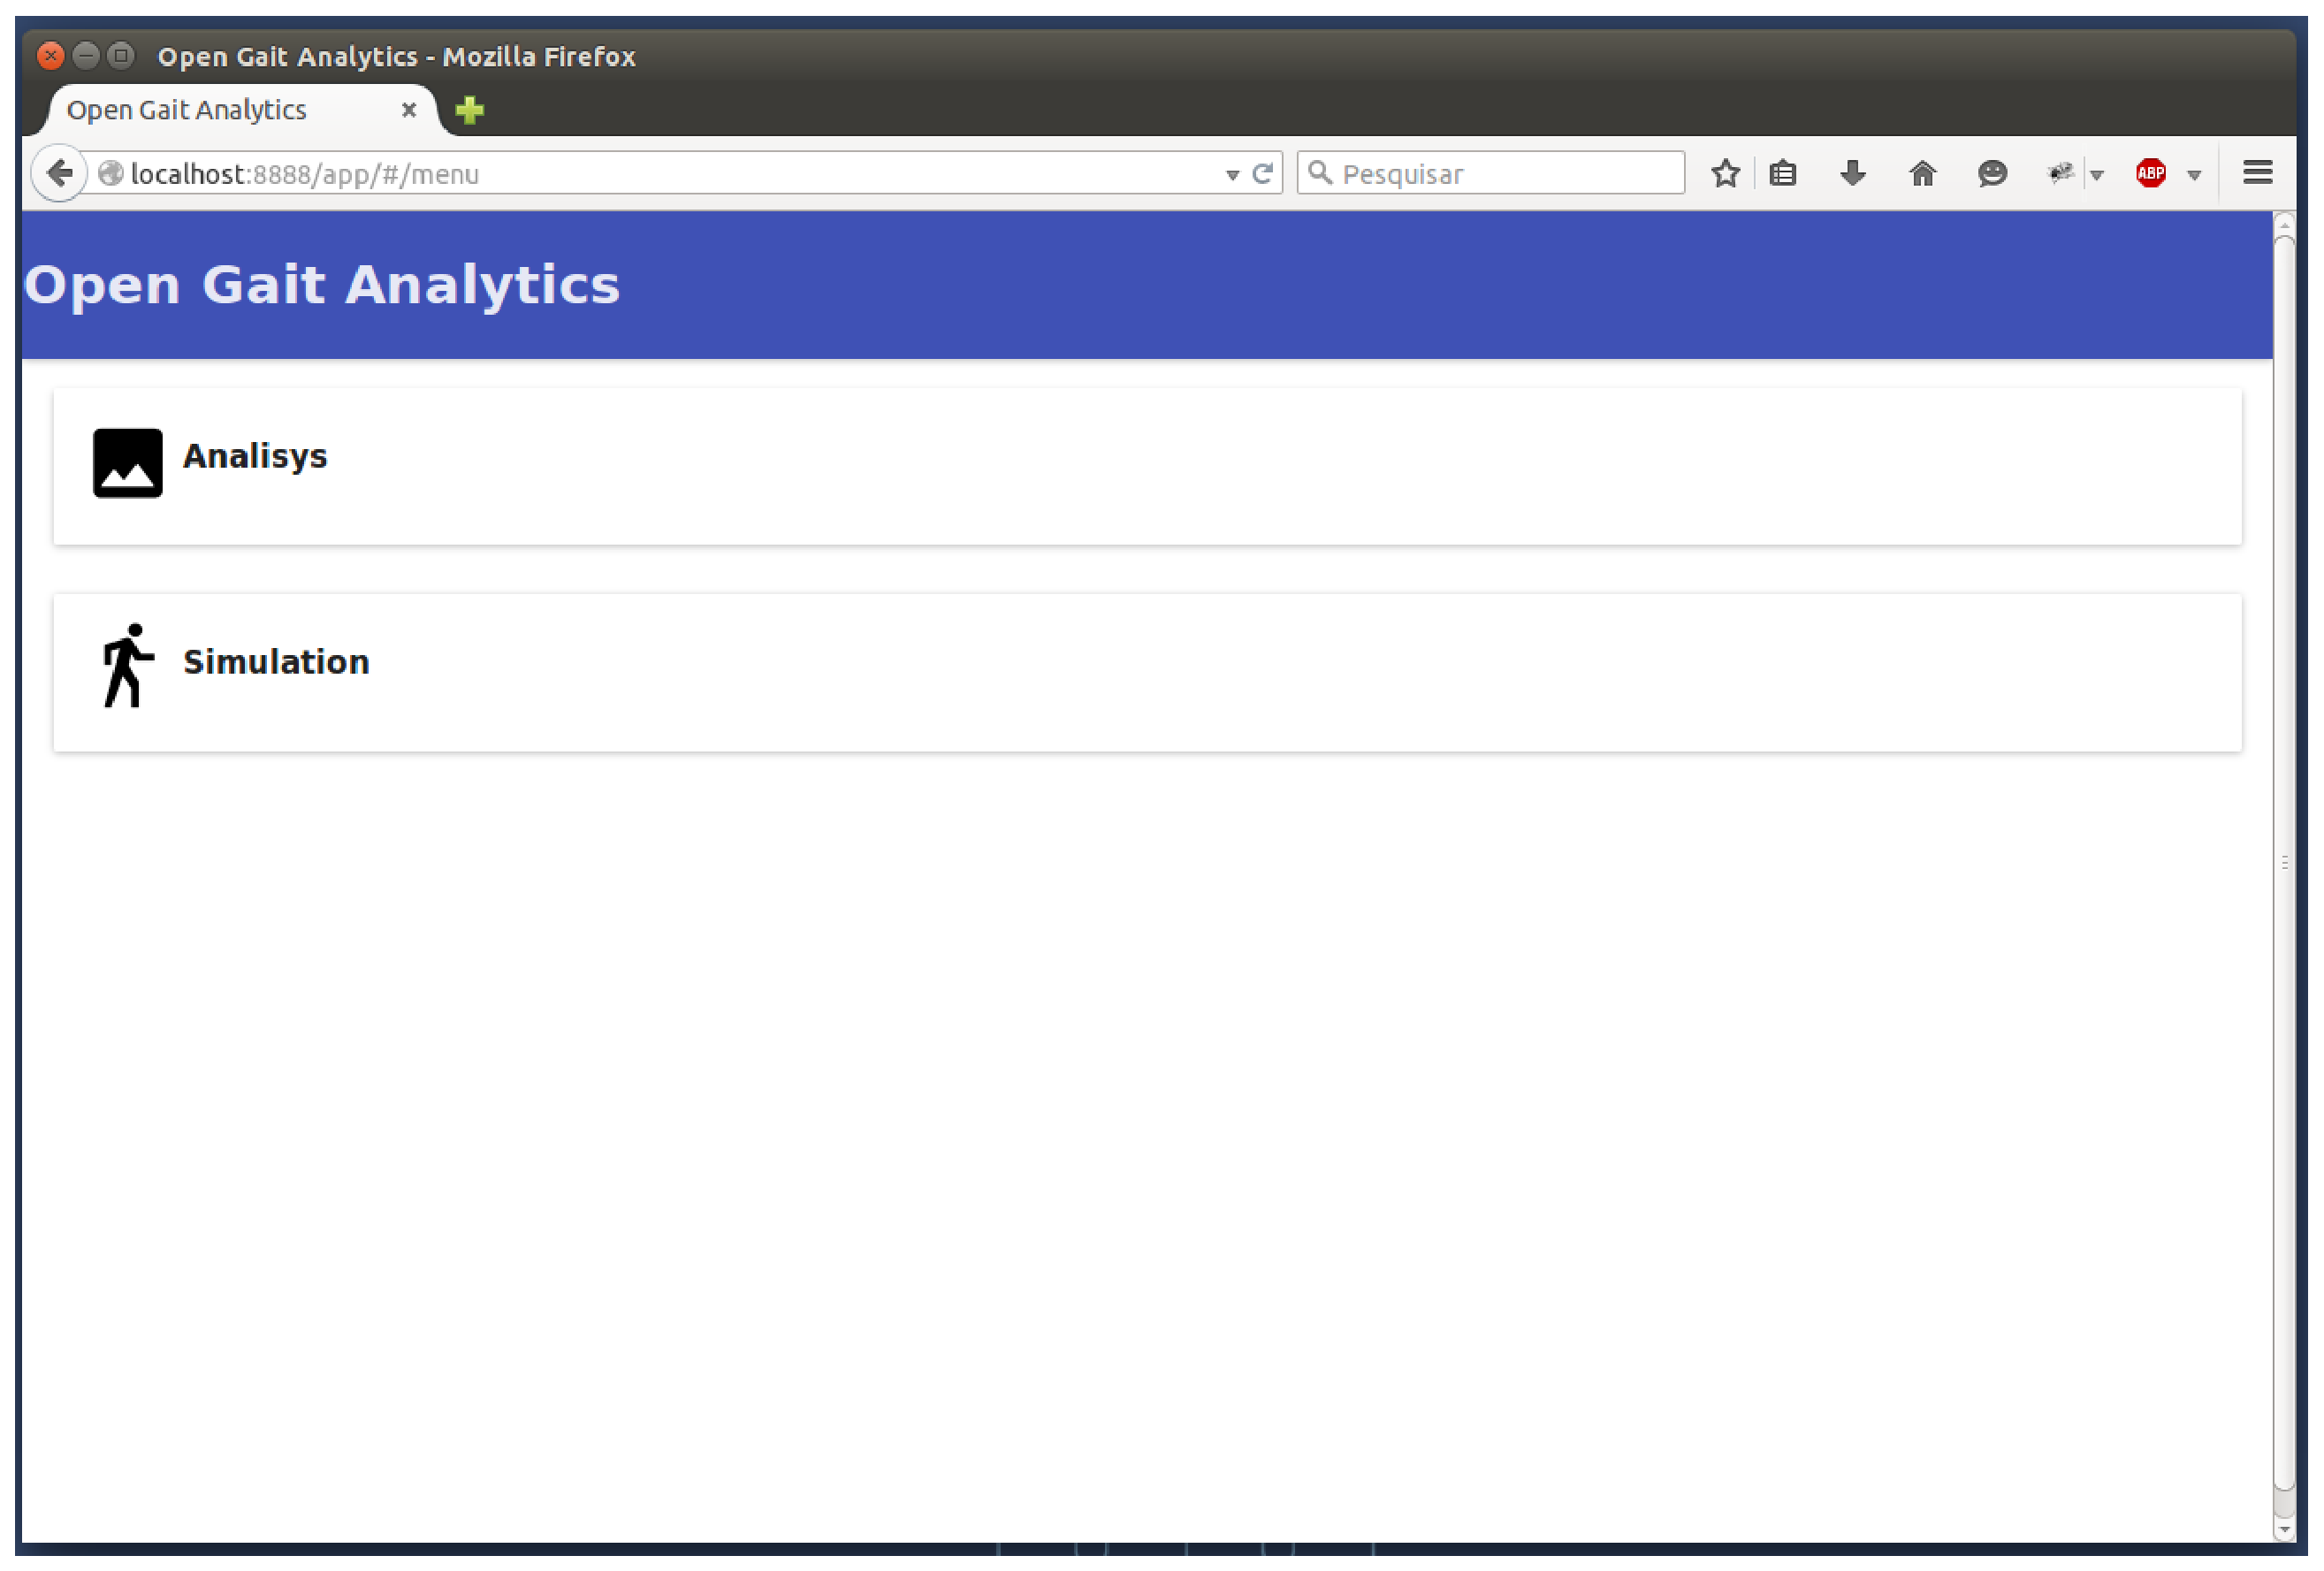
\includegraphics[width=15cm]{figuras/tela1.eps}
	\caption{Tela de seleção dos módulos.}
	\label{tela1}
\end{figure}

\section{Módulo de Análise}
Neste fase o software conta apenas com análise de movimentos, com sinais oriundos de marcadores passivos de superfície, captados por câmeras, usando o software \emph{QTM}. 
No \emph{QTM} é feita a conversão dos dados para o formato \emph{Matlab} que é reconhecido pelo sistema construído.

A primeira tela deste módulo pode ser vista na Figura \ref{tela2}. Este tela apresenta a listagem de pacientes, cadastrados no sistema. O botão abaixo a direita, é a função para adicionar novos pacientes.

\begin{figure}[H]
	\centering
	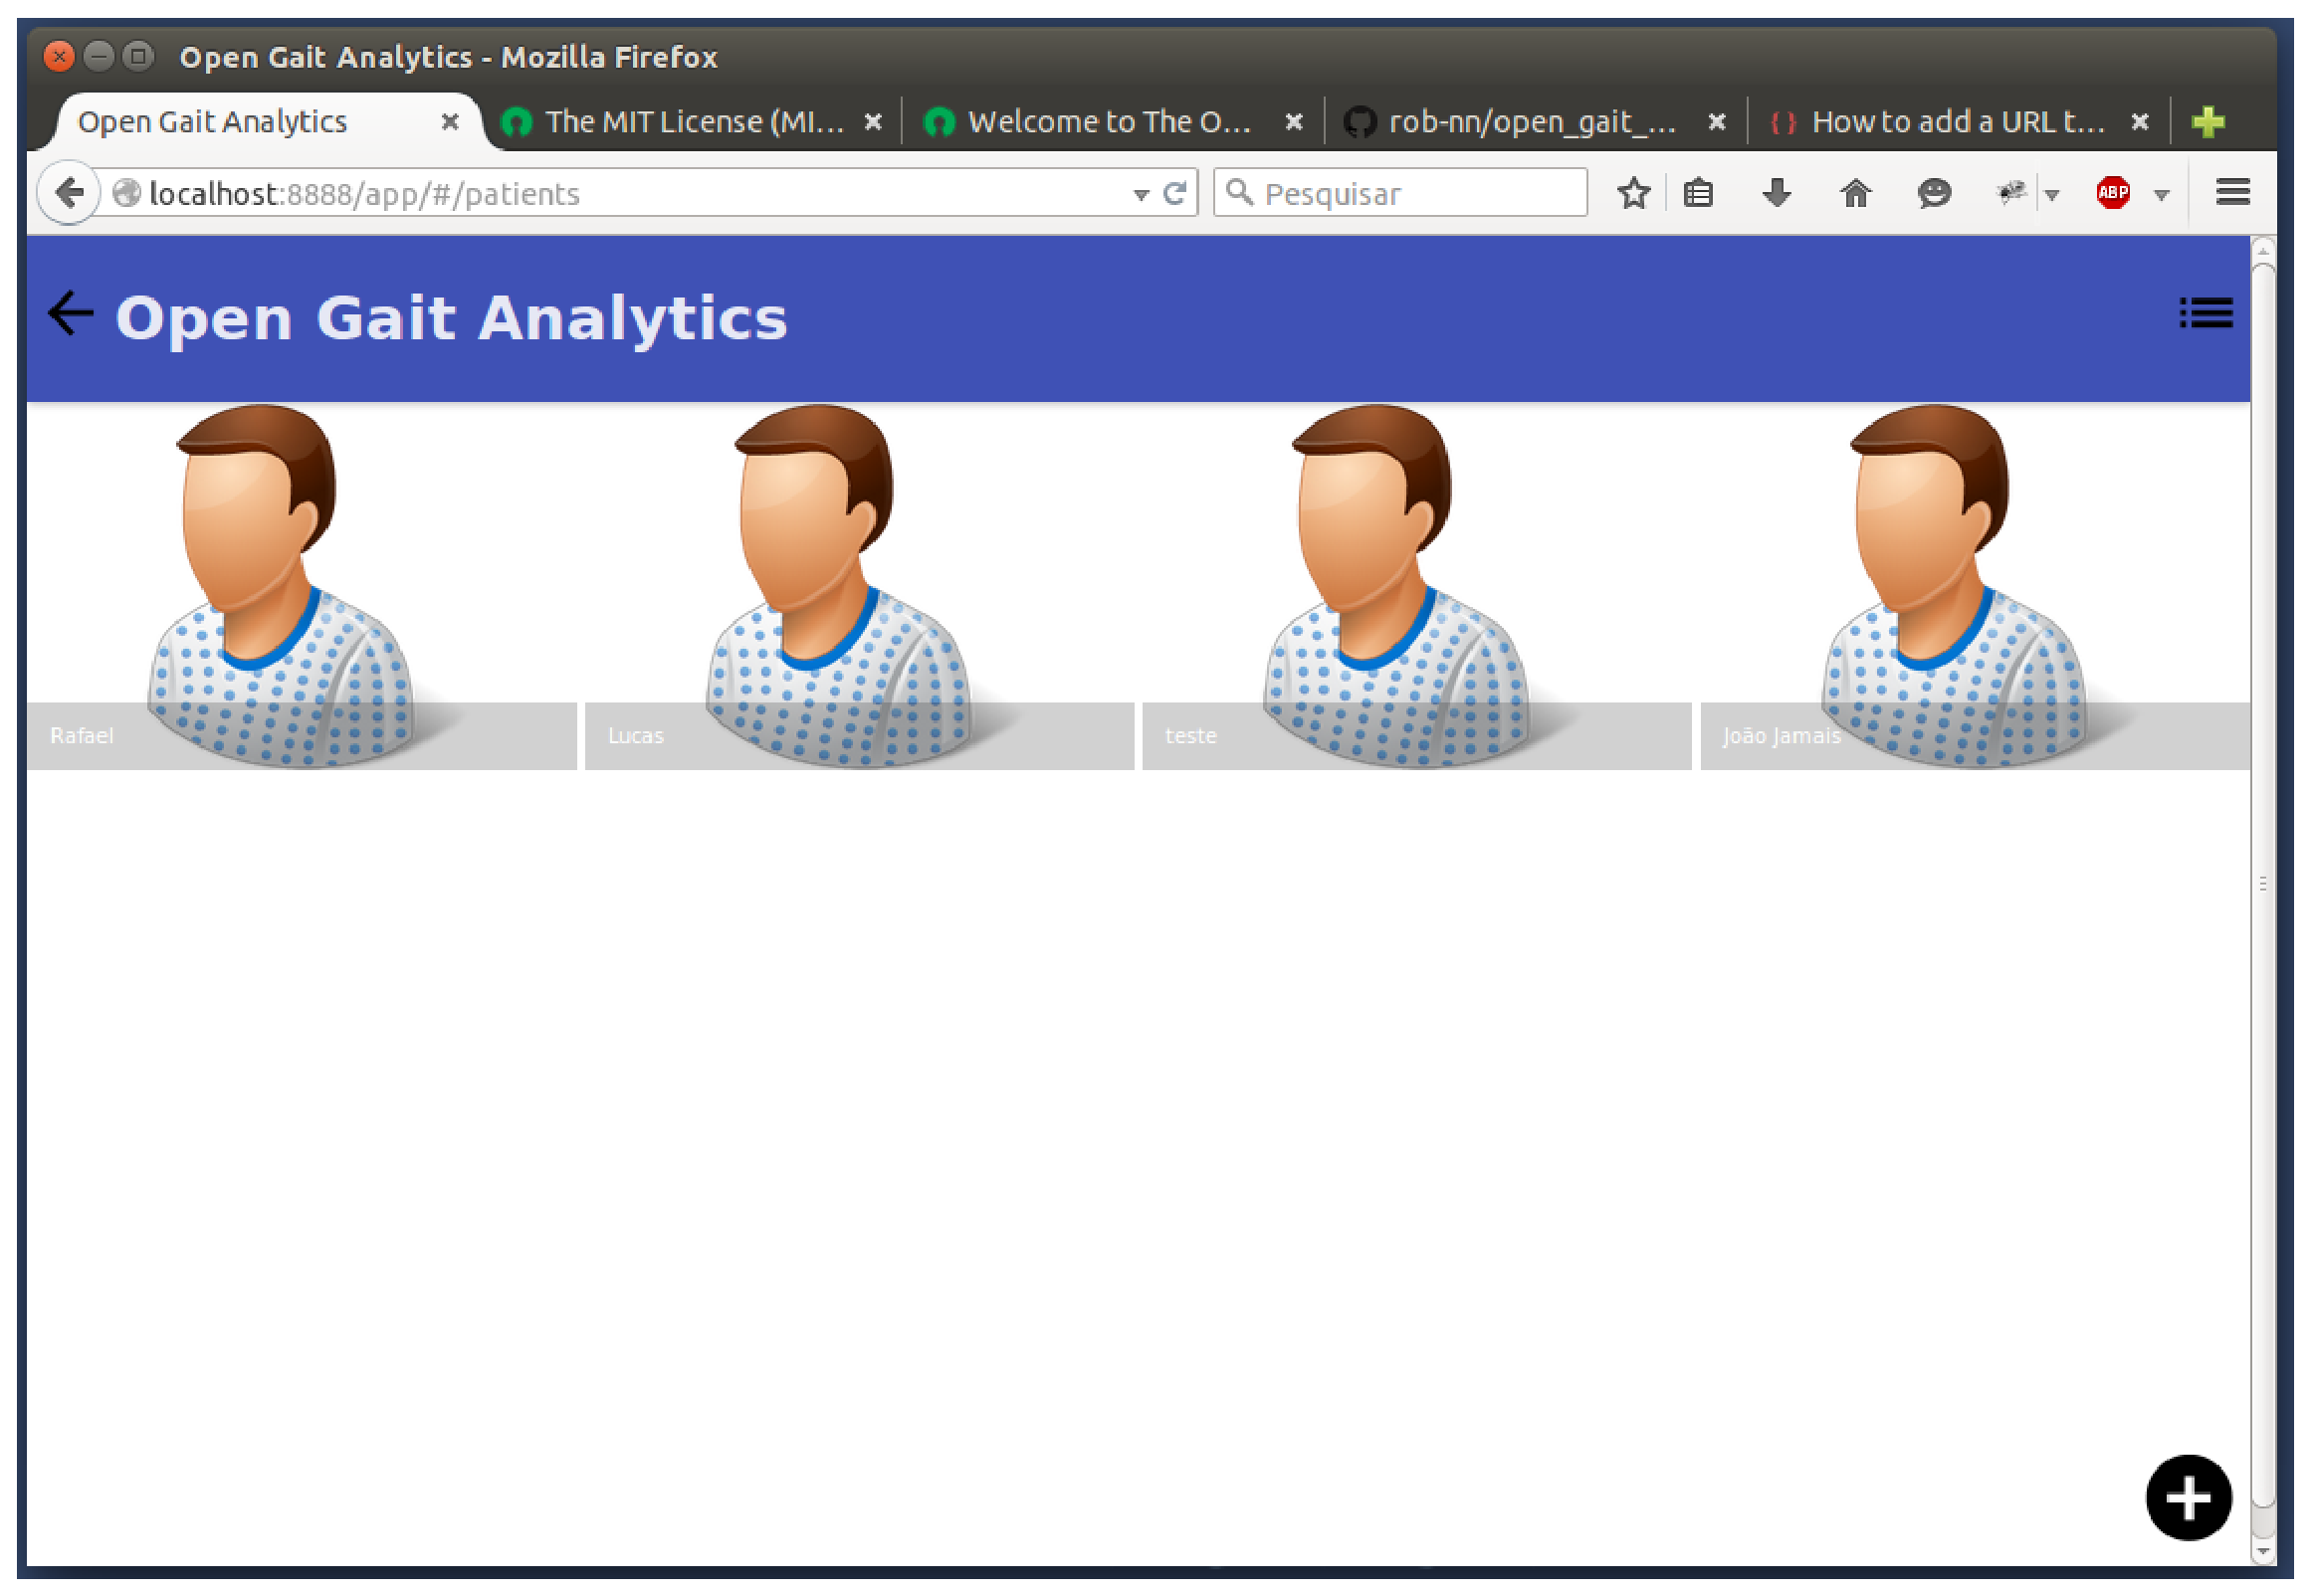
\includegraphics[width=15cm]{figuras/tela2.eps}
	\caption{Tela com a listagem de pacientes.}
	\label{tela2}
\end{figure}

A Figura \ref{tela3} mostra as informações do paciente que devem ser preenchidas ao se executar a função adicionar paciente. Esta tela é uma adaptação da ficha de avaliação que está na obra \citeonline{VeraReg}.

\begin{figure}[H]
	\centering
	\includegraphics[width=7cm]{figuras/tela3.eps}
	\caption{Informações do paciente.}
	\label{tela3}
\end{figure}

Ao se selecionar um paciente da tela mostrada na Figura \ref{tela2}, a tela da Figura \ref{tela4} aparece. No caso em questão, nenhuma coleta de dados foi carregada para o paciente. Logo, o próximo passo é adicionar uma nova amostra de marcha.
O usuário deve então informar a descrição da coleta e a data que a mesma ocorreu e salvar estas informações, conforme a Figura \ref{tela5}.

\begin{figure}[H]
	\centering
	\includegraphics[width=7cm]{figuras/tela4.eps}
	\caption{Tela inicial da dados coletados do paciente.}
	\label{tela4}
\end{figure}


\begin{figure}[H]
	\centering
	\includegraphics[width=15cm]{figuras/tela5.eps}
	\caption{Inclusão de amostra de marcha}

	\label{tela5}
\end{figure}



Depois de salva as informações o sistema pede para que o usuário selecione o arquivo proveniente do \emph{QTM}, conforme a Figura \ref{tela6}.
Depois de selecionado o arquivo com os dados da marcha, seus dados são mostrados para o usuário, conforme a Figura \ref{tela7}.

\begin{figure}[H]
	\centering
	\includegraphics[width=14cm]{figuras/tela6.eps}
	\caption{Seleção do arquivo no formato \emph{MATLAB} proveniente do \emph{QTM}.}
	\label{tela6}
\end{figure}
\begin{figure}[H]
	\centering
	\includegraphics[width=14cm]{figuras/tela7.eps}
	\caption{Dados do arquivo provenientes do \emph{QTM}.}
	\label{tela7}
\end{figure}





Neste momento, se o usuário quiser visualizar uma animação dos dados, basta clicar na seta negra que aponta para a direita que uma animação será mostra conforme a Figura \ref{animacao1}.
Esta animação foi construída usando a tecnologia \emph{ThreeJS}, resumida na seção \ref{threejs_sec}. Uma das grandes vantagens desta característica do software em relação ao \emph{QTM}, que também a possui, é o fato de que a animação está rodando num \emph{browser web} moderno, ou seja, qualquer um com um \emph{browser} assim pode vê-la sem precisar do \emph{QTM} instalado. 
Além do mais, como o projeto pode continuar, fica a critério dos usuários decidirem que novas características seriam interessantes, não somente nas animações, mas em todo o software.


\begin{figure}[H]
  \centering
  \begin{minipage}[b]{0.32\textwidth}
    \includegraphics[width=\textwidth]{figuras/tela8.eps}
  \end{minipage}
  \hfill
  \begin{minipage}[b]{0.32\textwidth}
    \includegraphics[width=\textwidth]{figuras/tela9.eps}
  \end{minipage}
  \hfill
  \begin{minipage}[b]{0.32\textwidth}
    \includegraphics[width=\textwidth]{figuras/tela10.eps}
  \end{minipage}
  \caption[Animação dos marcadores em 3D.]{Animação dos marcadores em 3D. A primeira figura mostra o contato inicial de uma perna. A segunda um momento no período de instância. A terceira o balanço terminal.}
  \label{animacao1}
\end{figure}


A tela da animação também possui controle de perspectivas 
(Figura \ref{animacao2}), controle de \emph{zoom} (Figura \ref{animacao3}), 
e controle \emph{pan} (Figura \ref{animacao4}).
Também foram implementados, até o momento, botões de \emph{play, pause}, fechar e um contador de \emph{frames} (Figura \ref{animacao5}).

\begin{figure}[H]
  \centering
  \begin{minipage}[b]{0.40\textwidth}
    \includegraphics[width=\textwidth]{figuras/tela11.eps}
  \end{minipage}
  \hfill
  \begin{minipage}[b]{0.40\textwidth}
    \includegraphics[width=\textwidth]{figuras/tela12.eps}
  \end{minipage}
  \caption[Controle de perspectivas.]{Controle de perspectivas. Primeira figura mostra uma perspectiva lateral do paciente. A segunda figura mostra uma perspectiva diagonal.}
  \label{animacao2}
\end{figure}

\begin{figure}[H]
  \centering
  \begin{minipage}[b]{0.49\textwidth}
    \includegraphics[width=\textwidth]{figuras/tela13.eps}
  \end{minipage}
  \hfill
  \begin{minipage}[b]{0.49\textwidth}
    \includegraphics[width=\textwidth]{figuras/tela14.eps}
  \end{minipage}
  \caption[Controle de \emph{zoom}.]{Controle de \emph{zoom}. Primeira figura \emph{zoom out}. Segunda figura \emph{zoom in}.}
  \label{animacao3}
\end{figure}

\begin{figure}[H]
  \centering
  \begin{minipage}[b]{0.49\textwidth}
    \includegraphics[width=\textwidth]{figuras/tela15.eps}
  \end{minipage}
  \hfill
  \begin{minipage}[b]{0.49\textwidth}
    \includegraphics[width=\textwidth]{figuras/tela16.eps}
  \end{minipage}
  \caption[Controle \emph{pan}.]{Controle \emph{pan}. Primeira figura mostra o paciente mais a direita e embaixo. A segunda figura mostra o paciente mais a esquerda e acima.}
  \label{animacao4}
\end{figure}

\begin{figure}[ht]
	\centering
	\includegraphics[width=7cm]{figuras/tela17.eps}
	\caption{Controles da animação.}
	\label{animacao5}
\end{figure}






É de fundamental importância que o usuário configure os parâmetros \emph{Initial Contact} e \emph{Terminal Swing} mostrados na Figura \ref{tela7}. Sem estes parâmetros os gráficos, vão mostrar os sinais nas fases erradas do ciclo de marcha.
A técnica que se recomenda é inicializar a animação e quando o usuário perceber o \emph{initial contact}, pressionar o botão \emph{pause} e anotar o \emph{frame}. Fazer a mesma coisa para o \emph{terminal swing}.

Outra opção disponível na Figura \ref{tela7} é a opção \emph{Markers}, esta opção permite nomear os marcadores e visualizar sua progressão espacial. 
A Figura \ref{tela18} mostra o resultado de se selecionar esta opção.
Ao clicar no botão ao lado de algum marcador, sua progressão no espaço é mostrada num gráfico como o da Figura \ref{tela19}. O domínio é o percentual do ciclo de marcha, já a imagem são dados espaciais brutos oriundos do \emph{QTM}.

\begin{figure}[H]
	\centering
	\includegraphics[width=4cm]{figuras/tela18.eps}
	\caption{Opção \emph{markers}.}
	\label{tela18}
\end{figure}


\begin{figure}[H]
	\centering
	\includegraphics[width=10cm]{figuras/tela19.eps}
	\caption{Progressão espacial de um marcador.}
	\label{tela19}
\end{figure}

A nomeação dos marcadores, não é uma tarefa trivial. Para isso foi criada uma ferramenta dentro da animação para ajudar com esta tarefa. Primeiro, deve-se entrar na animação, depois pausá-la, e posicionar a visualização de uma forma que ajude a detectar o marcador procurado. Veja a Figura \ref{tela20}, nela um marcador foi clicado com o \emph{mouse}, o marcador ficou azul e ao seu lado ele mostra o índice 30. 
Agora é só voltar na opção de marcadores, procurar o índice 30 (\emph{Marker 30}) e colocar o nome desejado. No caso deste marcador o nome é joelho esquerdo (\emph{left knee}, Figura \ref{tela21}).
Agora para o sistema o marcador 30 é sempre o joelho esquerdo (Figura \ref{tela22}).

\begin{figure}[H]
	\centering
	\includegraphics[width=5cm]{figuras/tela20.eps}
	\caption{Seleção de um marcador pelo \emph{mouse}.}
\label{tela20}
\end{figure}

\begin{figure}[H]
	\centering
	\includegraphics[width=7cm]{figuras/tela21.eps}
	\caption{Renomeando um marcador.}
\label{tela21}
\end{figure}
\begin{figure}[H]
	\centering
	\includegraphics[width=5cm]{figuras/tela22.eps}
	\caption{Animação mostrando o marcador renomeado.}
\label{tela22}

\end{figure}



Outra funcionalidade importante é o gerador de ângulos. Esta opção está disponível na Figura \ref{tela7}. E após selecionada é mostrada na Figura \ref{tela23}. 
Para se gerar um ângulo, o usuário necessita selecionar a opção de inclusão de ângulo e preencher os dados da Figura \ref{tela24}. O usuário precisa indicar a origem do ângulo, por exemplo, o joelho, o componente A, por exemplo, algum músculo da coxa, e o componente B, por exemplo, a tíbia. Estes pontos poderiam representar o ângulo de um joelho, por exemplo.
\begin{figure}[H]
	\centering
	\includegraphics[width=15cm]{figuras/tela23.eps}
	\caption{Opção de visualização e criação de ângulos.}
\label{tela23}
\end{figure}


\begin{figure}[H]
	\centering
	\includegraphics[width=15cm]{figuras/tela24.eps}
	\caption{Inclusão de um novo ângulo.}
\label{tela24}
\end{figure}


Depois dos ângulos criados é possível ver seus valores durante o ciclo de marcha ou suas velocidades angulares, conforme as Figuras \ref{tela25} e \ref{tela26}.
Os ângulos são criados conforme as fórmulas que estão na Seção \ref{cinematica}. O número de pontos usados para o cálculo depende dos parâmetros informados e da quantidade de \emph{frames} por segundo configurada no \emph{QTM}.
\begin{figure}[H]
	\centering
	\includegraphics[width=8cm]{figuras/tela25.eps}
	\caption{Ângulo de um joelho durante o ciclo de marcha.}
\label{tela25}
\end{figure}

\begin{figure}[H]
	\centering
	\includegraphics[width=8cm]{figuras/tela26.eps}
	\caption{Velocidades angulares de um joelho durante o ciclo de marcha.}
\label{tela26}
\end{figure}


\section{Módulo de Simulação}
Este módulo é sem dúvida o que mais vai contribuir para os pesquisadores, pois estes contarão com a base integrada gerada pelo módulo de análise e com estas informações será possível realizar simulações de sinais e classificações. 
A versão atual do software ainda é muito pobre neste quesito, mas o objetivo neste momento é mostrar a viabilidade de se usar algoritmos de sistemas inteligentes, integrados na base que vai sendo gerada.
Acredita-se que a ferramenta vai ser mais apreciada por pesquisadores que tem como formação a área de saúde, pois estes não precisarão de todas as técnicas exigidas para fazer simulações num ambiente como o do \emph{MATLAB}.

A primeira funcionalidade de simulação que foi implantada foi a simulação pela \emph{CMAC}, em que esta RNA foi descrita na seção \ref{cmac_sec}. 
Ao se selecionar o módulo simulação, a tela da Figura \ref{tela27} é apresentada. 
A opção \emph{CMAC} já aparece selecionada. 
Para efeitos da demonstração das funcionalidades deste módulo foi realizada uma simulação das velocidades angulares de um joelho, a partir de outros sinais disponíveis.

\begin{figure}[H]
	\centering
	\includegraphics[width=10cm]{figuras/tela27.eps}
	\caption{Módulo de simulação.}
\label{tela27}
\end{figure}


Após ser selecionado o nome de um paciente, deve-se selecionar uma amostra de ciclo de marcha (Figura \ref{tela28}).
Após a seleção do ciclo de marcha, uma lista com vários sinais são mostrados, basicamente os sinais são coordenadas de posições de marcadores, ângulos e velocidades angulares. As Figuras \ref{tela29} e \ref{tela30} mostram uma fração dos sinais possíveis para seleção. Ao se selecionar um sinal de entrada é necessário também informar sua quantização.
\begin{figure}[H]
	\centering
	\includegraphics[width=10cm]{figuras/tela28.eps}
	\caption{Seleção do ciclo de marcha.}
\label{tela28}
\end{figure}

\begin{figure}[H]
	\centering
	\includegraphics[width=5cm]{figuras/tela29.eps}
	\caption{Sinais de entrada para a \emph{CMAC}. No caso posições num plano 3D de marcadores.}
\label{tela29}
\end{figure}

\begin{figure}[H]
	\centering
	\includegraphics[width=5cm]{figuras/tela30.eps}
	\caption{Sinais de entrada para a \emph{CMAC}, ângulos e velocidades angulares.}
\label{tela30}
\end{figure}


A Figura \ref{tela31} mostra uma configuração que gera a saída da Figura \ref{tela32}.  O gráfico mostrado é a saída da RNA  \emph{CMAC}. 
A Figura \ref{tela33} mostra o erro quadrado médio da execução da simulação ao longo das iterações.
\begin{figure}[H]
	\centering
	\includegraphics[width=10cm]{figuras/tela31.eps}
	\caption{Exemplo de configuração para uma simulação usando \emph{CMAC}.}
\label{tela31}
\end{figure}

\begin{figure}[H]
	\centering
	\includegraphics[width=10cm]{figuras/tela32.eps}
	\caption{Resultado da simulação.}
\label{tela32}
\end{figure}

\begin{figure}[H]
	\centering
	\includegraphics[width=10cm]{figuras/tela33.eps}
	\caption{Erro quadrado médio em cada iteração da simulação.}
\label{tela33}
\end{figure}

\section{Uso do sistema em dispositivos móveis}
Uma das maiores vantagens nas tecnologia escolhidas para compor a camada web, é sua total compatibilidade com dispositivos móveis capazes de executar \emph{browsers} modernos como \emph{Firefox, Chrome ou Safari}. O \emph{angular-material} já apresenta comportamentos muito bons em dispositivos de pequenas telas. 
Veja um exemplo nas Figuras \ref{tela34} e \ref{tela35} da aplicação rodando no \emph{browser} \emph{Firefox}, num dispositivo \emph{Motorola Xoom}. A Figura \ref{tela36} mostra a aplicação rodando em um \emph{iPhone4} com \emph{browser Safari}.

\begin{figure}[H]
	\centering
	\includegraphics[width=12cm]{figuras/tela34.eps}
	\caption{Aplicação \emph{Open Gait Analytics} rodando num \emph{browser Firefox} e dispositivo \emph{Motorola Xoom}.}
\label{tela34}
\end{figure}

\begin{figure}[H]
	\centering
	\includegraphics[width=12cm]{figuras/tela35.eps}
	\caption{Animação de uma amostra de marcha rodando num \emph{browser Firefox} e dispositivo \emph{Motorola Xoom}.}
\label{tela35}
\end{figure}

\begin{figure}[H]
	\centering
	\includegraphics[width=5.5cm]{figuras/tela36.eps}
	\caption{Aplicação rodando num \emph{iPhone 4} com \emph{browser Safari}.}
\label{tela36}
\end{figure}


Para frisar como a aplicação se adapta inteligentemente ao dispositivo que está rodando, compare a Figura \ref{tela34} com a Figura \ref{comp1}. 
Veja que a barra lateral desaparece na tela menor do \emph{iPhone 4}. Em cima da tela aparece a opção \emph{open side} que quando clicada mostra a barra lateral por cima do formulário.
\begin{figure}[H]
  \centering
  \begin{minipage}[b]{0.35\textwidth}
    \includegraphics[width=\textwidth]{figuras/tela37.eps}
  \end{minipage}
  \hfill
  \begin{minipage}[b]{0.35\textwidth}
    \includegraphics[width=\textwidth]{figuras/tela38.eps}
  \end{minipage}
  \caption{Adaptação da aplicação em telas pequenas.}
  \label{comp1}
\end{figure}


Para o profissional de saúde, este é um recurso a mais, pois agora do seu próprio celular e em qualquer lugar ele poder ver dados dos seus pacientes.



\chapter[DISCUSSÃO E CONCLUSÃO]{\textbf{DISCUSSÃO E CONCLUSÃO}}

Há vários softwares de análise de marcha no mercado, mas a ideia de criar um totalmente na \emph{web} tem suas vantagens. 
A mais óbvia é a disponibilidade, já que a aplicação fica num servidor na \emph{internet}, isto é, o usuário só precisa acessar um \emph{site} com um \emph{browser}. 
Outra não tão óbvia e que diz respeito principalmente ao módulo de simulação, é a possibilidade de escalar a aplicação para necessidades de processamento gigantescas, usando infraestrutura como serviço de fornecedores como o \emph{Microsoft Azure} ou \emph{Amazon Webservices}.
Como a camada \emph{web} se comunica via \emph{HTTP} no estilo \emph{REST}, usando uma \emph{facade} para isto, basta fazer a \emph{facade} do módulo de simulação apontar para uma \emph{web farm} alocada sob demanda num dos serviços mencionados. 
A vantagem óbvia é que quem serve a aplicação, pode alocar estes serviços sob demanda, não necessitando possuir um Centro de Processamento de Dados (CPD) caríssimo. O custo é repassado ao cliente que deseja usar os serviços de simulação que demandam muito poder de processamento.

Outro ponto interessante com a implantação da aplicação é a criação de uma base de dados de marcha humana, que pode receber dados de todo o globo. 
As vantagens para pesquisadores da área de análise de marcha seriam inimagináveis.

Claro que nada disto é gratuito, os responsáveis pelo projeto terão de almejar meios para produzi-lo, achar nichos de mercado e colocá-lo em produção.

Ressalta-se, novamente, que o software que está sendo entregue não está pronto para a produção. O prazo disponível para desenvolvê-lo, inclusive adquirindo conhecimentos sobre muitas das tecnologias adotadas, foi de aproximadamente cinco meses. 
Isto ocorreu porque durante o programa de mestrado resolveu-se mudar o tema, devido a uma série de intempéries. No entanto, o software foi feliz em mostrar a integração de vários componentes nas diferentes camadas da aplicação. O ato de estressar a arquitetura é muito importante para se avaliar a viabilidade técnica de um projeto de engenharia de software.

Outro problema com o software entregue, é seu modesto poder de processamento com relação a simulações. 
Facilmente uma simulação em um grande \emph{Data Center} pode demorar dias. 
A solução para este problema é desenvolver um método para disparar a simulação assincronamente, bem como criar uma tela de gestão da execução da mesma. 
Para isso, o software terá de ser integrado a componentes de computação distribuída como \emph{Apache Spark} ou o \emph{Hadoop}, fazendo uso de infraestrutura como serviço conforme mencionado anteriormente. 
O potencial para este projeto se tornar algo inovador e, principalmente, muito útil na área de marcha humana é imenso.

Talvez o objetivo que tenha sido mais prejudicado, foi a implantação do método ágil. 
Como o método escolhido foi o \emph{SCRUM} e não foi possível criar as reuniões diárias \emph{(daily scrum)}, a dinâmica da equipe não foi a mesma em que o autor teve a oportunidade de trabalhar com outras equipes.
Recomenda-se também, que uma equipe de especialistas clínicos e pesquisadores da área da marcha humana sejam adicionados ao projeto e ajudem ao \emph{product owner} do projeto a definir novas funcionalidades para o sistema. 
Isso certamente vai acelerar a adoção do software por estes profissionais, já que são as necessidades deles que serão atingidas.
Talvez um projeto de \emph{crowdfunding} possa trazer estes profissionais. 
É comum nestes projetos os clientes pedirem funcionalidades para o software.
O problema é que este é um software para um nicho muito especializado, pode ser que não seja uma boa ideia.


A questão dos testes também foi um pouco prejudicada, mas não abandonada. Na verdade esta foi uma escolha do autor, que devido ao pouco tempo para desenvolvimento, preferiu dar ênfase na produção de novas características. Mesmo assim todos os principais componentes, como a \emph{web API} e os componentes de telas da análise de marcha, possuem testes automatizados.
A consequência é que \emph{bugs} menores como listas de seleção podem aparecer fora dos locais adequados, o componente de controle de animação as vezes fica com um tamanho inadequado, mas não é nada que com os recursos adequados não se resolva.

Vale lembrar também que o projeto não vai se limitar a análise de movimento. 
Outros métodos de coleta de dados para análise serão inseridos ao longo do tempo, por exemplo, IMU.


Concluindo, os objetivos foram alcançados, foi definida uma metodologia ágil, foi criado um modelo de arquitetura, um software foi construído, integrado com os principais componentes e, na medida do possível testados, e mais uma vez, frisando que toda a arquitetura foi estressada. 
Além disso, a aplicação ainda apresenta características para serem executadas em dispositivos móveis. 
Uma ferramenta de análise de movimento com várias funcionalidades foi construída, assim como uma simulação usando a \emph{CMAC}.
Também o código fonte com todo o histórico de desenvolvimento do projeto, inclusive histórias do usuário, estão no \emph{site} \url{https://github.com/rob-nn/open\_gait\_analytics}, lembrando que o código está sob licença MIT (Anexo \ref{licenca_mit}), e qualquer um pode usá-lo conforme a necessidade.


\chapter[TRABALHOS FUTUROS]{\textbf{TRABALHOS FUTUROS}}
Como este foi um projeto com um intuito de plantar uma semente, não faltarão trabalhos futuros para complementá-lo, aumentá-lo ou mesmo expandi-lo para outras áreas além da análise de marcha. Além disso, o projeto conta com um \emph{backlog} de produto sempre evoluindo, o que é uma fonte de trabalhos futuros constante.
\begin{enumerate}
	\item O trabalho mais urgente a ser feito é usar a versão atual, testá-la o máximo possível, corrigir os \emph{bugs} encontrados e disponibilizá-la na \emph{web};
	\item Inserir o padrão ouro nos gráficos para efeito de comparação;
	\item Criar no módulo de simulação uma ferramenta para modelagem de sinais de entrada, métodos de processamento e sinais de saída, baseados nos dados da base de documentos;
	\item Habilitar o protocolo \emph{HTTP Auth} nas requisições feitas a \emph{web API};
	\item Habilitar protocolo \emph{HTTPS} entre servidor \emph{web} e \emph{browser} cliente;
	\item Implementar um detector automático de ciclo de marcha, assim não será necessário o usuário informar o início e o fim do ciclo;
	\item Permitir cadastrar protocolos de coleta por câmeras e fazer a detecção automática dos mesmos, assim o usuário não necessitará nomear marcadores;
	\item Permitir coletar dados de plataforma de força e criar gráficos;
	\item Permitir coletar dados de \emph{IMUs} e criar gráficos;
	\item Permitir coletar dados de \emph{EMGs} e criar gráficos;
	\item Permitir coletar dados de eletrogoniômetros;
	\item Criar suporte a várias línguas, começando com português e inglês;
	\item Implementar outros algoritmos de sistemas inteligentes, como \emph{Pricipal Component Analysis (PCA)}, \emph{Kmeans}, \emph{Suport Vector Machine (SVM)}, \emph{Multi Layer Perceptron (MLP)} \cite{Haykin1998}, entre outros, integrando estes algoritmos a ferramenta de modelagem de sinais, permitindo se fazer classificações e regressões. 
Por exemplo, usando-se \emph{SVM} é possível fazer a detecção de quedas, ou usando o Kmeans é possível detectar os momentos distintos no uso de uma plataforma de força. 
Aqui o que vai imperar é a criatividade do pesquisador, que terá nas mãos uma ferramenta visual para fazer estas simulações. 
A evolução desse módulo acontecerá quando as simulações forem úteis o suficiente para auxiliar nos diagnósticos de patologias na marcha. 
Com a tecnologia atual de aprendizado de máquina, as possibilidades são muito atrativas.
	\item Integrar o módulo de simulação com plataformas de infraestrutura com serviço, usando para isso ferramentas como \emph{Hadoop} ou \emph{Spark};
	\item Tornar a função de execução de simulações assíncronas;
	\item Criar um módulo gestor da execução das simulações, com opções de parar, pausar, continuar, alocar mais recursos, enfileiramento;
	\item Criar uma ferramenta para extração de dados com possibilidade de criar filtros nos dados espaciais.
\end{enumerate}




\bookmarksetup{startatroot} 
\postextual

\renewcommand{\bibname}{\textbf{REFERÊNCIAS BIBLIOGRÁFICAS}\hfill} % Altera o nome da Referêcia para Referêcia Bibliográfica
\bibliography{bibliografia}
\printindex

\end{document}
